\documentclass[12pt,a4paper]{report}

% ---------------------------
% Page layout and formatting
% ---------------------------
\usepackage[utf8]{inputenc}
\usepackage[T1]{fontenc}
\usepackage{lmodern}
\usepackage[a4paper,margin=1in]{geometry}
\usepackage{setspace}
\usepackage{parskip}
\usepackage{fancyhdr}
\usepackage{url}
% ---------------------------
% Mathematics
% ---------------------------
\usepackage{amsmath}
\usepackage{amssymb}
\usepackage{amsthm}
\usepackage{bm}

% ---------------------------
% Figures, tables, captions
% ---------------------------
\usepackage{graphicx}
\usepackage{float}
\usepackage{booktabs}
\usepackage{multirow}
\usepackage{array}
\usepackage{caption}
\usepackage{subcaption}

% ---------------------------
% Colors and code listings
% ---------------------------
\usepackage{xcolor}
\usepackage{listings}

\definecolor{codebg}{RGB}{245,245,244}
\definecolor{codecomment}{RGB}{0,128,0}
\definecolor{codekeyword}{RGB}{0,0,180}
\definecolor{codestring}{RGB}{163,21,21}

\lstdefinestyle{mystyle}{
	backgroundcolor=\color{codebg},
	commentstyle=\color{codecomment},
	keywordstyle=\color{codekeyword}\bfseries,
	stringstyle=\color{codestring},
	basicstyle=\ttfamily\small,
	breakatwhitespace=false,
	breaklines=true,
	captionpos=b,
	keepspaces=true,
	numbers=left,
	numbersep=8pt,
	numberstyle=\tiny\color{gray},
	showspaces=false,
	showstringspaces=false,
	showtabs=false,
	tabsize=4,
	frame=single
}
\lstset{style=mystyle}

% ---------------------------
% Hyperlinks and references
% ---------------------------
\usepackage{hyperref}
\usepackage[nameinlink,noabbrev]{cleveref}

\hypersetup{
	colorlinks=true,
	linkcolor=blue,
	citecolor=blue,
	urlcolor=blue,
	pdftitle={Confidence-Weighted Multi-Scale Rolling Forecasting of Urban Taxi Demand with GraphSAGE-Based Spatial Refinement},
	pdfauthor={Tianqi Wang}
}

% ---------------------------
% Bibliography
% ---------------------------
\usepackage[backend=biber,style=ieee]{biblatex}
\addbibresource{reference.bib}

% ---------------------------
% Optional utilities
% ---------------------------
\usepackage{enumitem}
\usepackage{longtable}
\usepackage{pdflscape}

% ---------------------------
% Header / Footer
% ---------------------------
\pagestyle{fancy}
\setlength{\headheight}{15pt}
\fancyhf{}
\fancyhead[L]{MSc Thesis}
\fancyhead[R]{\leftmark}
\fancyfoot[C]{\thepage}

% ---------------------------
% Theorem environments
% ---------------------------
\newtheorem{theorem}{Theorem}[chapter]
\newtheorem{definition}{Definition}[chapter]

% ---------------------------
% Document starts here
% ---------------------------
\begin{document}
	
	% ---------------------------
	% Title page
	% ---------------------------
	\begin{titlepage}
		\centering
		\vspace*{2cm}
		
		{\Huge\bfseries Confidence-Weighted Multi-Scale Rolling Forecasting of Urban Taxi Demand with GraphSAGE-Based Spatial Refinement\par}
		\vspace{1.5cm}
		
		{\Large Tianqi Wang\par}
		\vspace{0.5cm}
		{\large Master of Science by Research\par}
		\vspace{0.3cm}
		{\large University of Warwick\par}
		{\large Department of Computer Science\par}
		\vspace{1.5cm}
		
		{\large Supervisor: Professor Ligang He\par}
		\vfill
		
		{\large Submitted in partial fulfilment of the requirements\\
			for the degree of Master of Science by Research\par}
		
		\vspace{1cm}
		{\large July 2026\par}
	\end{titlepage}
	
	% ---------------------------
	% Front matter
	% ---------------------------
	\pagenumbering{roman}
	
	\tableofcontents
	\clearpage
	\listoffigures
	\addcontentsline{toc}{chapter}{List of Figures}
	\clearpage
	\listoftables
	\addcontentsline{toc}{chapter}{List of Tables}
	\clearpage

	\chapter*{Acknowledgements}
	\addcontentsline{toc}{chapter}{Acknowledgements}
	First of all, I would like to express my sincere gratitude to my Dissertation supervisor,     
	\textbf{Professor Ligang He}, for his meticulous guidance and selfless help in the process of topic selection, research design, and thesis writing. When I encountered difficulties, he patiently pointed me in the right direction and offered valuable academic advice.
	
	I am also grateful to the senior members of Professor He's research group for their support and inspiration in data processing, experimental tuning, model implementation, and code debugging: \textbf{Yan Qian}, \textbf{Da Yan}, \textbf{Xuan Huang}, \textbf{Weitong Liao}, \textbf{Stephen Xu}, \textbf{Ashley Au}, \textbf{Xiao Qin}, \textbf{Zhihao Dai}, \textbf{Yiming Wei}, \textbf{Xuanyu Liu}, \textbf{Yuchen Liu}, \textbf{Yi Su}, and \textbf{Peng Jiang}.
	
	My thanks go to the open source community and the developers of tools such as PyTorch, PyTorch Geometric, Pandas, and NumPy, whose generously shared code and documentation made this research far more efficient.
	
	Finally, I would like to thank my family and my girlfriend, Yuanting Shi, for their understanding and support throughout my academic journey. Their encouragement has allowed me to focus on my research and continue moving forward.
	
	\clearpage
	\chapter*{Declaration}
	\addcontentsline{toc}{chapter}{Declaration}
	This thesis is submitted to the University of Warwick in support of my application for the degree of Master of Science by Research. It has been composed by myself and has not been submitted in any previous application for a degree or other qualification.

	The work presented, including data processing, implementation, experiments, analysis, and the preparation of this thesis, was carried out by Tianqi Wang under the academic supervision of Professor Ligang He. Professor He provided supervisory guidance, methodological advice, and feedback on the research and manuscript.

	Parts of the work reported in this thesis have been submitted as a workshop paper to ICA3PP 2026 and are currently under review.

	\clearpage

	\chapter*{Abstract}
	\addcontentsline{toc}{chapter}{Abstract}
Accurate urban taxi demand forecasting is essential for intelligent transportation management, fleet dispatching, and congestion mitigation. This thesis proposes a temporal-first framework for hourly prediction over New York City Taxi Zones. A temporal model produces a zone-level base forecast from observations available before the target hour; a GraphSAGE module then learns a residual correction from labelled residual snapshots that also precede that hour. This causal separation avoids training the graph model on target-hour labels. The study evaluates SARIMA, linear, recurrent, Transformer, PatchTST, TCN, and multi-scale temporal backbones under the same twelve rolling 24-hour windows. TCN is selected for the causal residual experiments because it is slightly lower than multi-scale on MAE, RMSE, and MSE, although the two are competitive. The thesis develops and evaluates a multi-scale temporal candidate as a substantive methodological component; TCN is selected only as the fixed temporal backbone for the subsequent causal residual experiments. Confidence combines historical support, Monte Carlo Dropout stability, and historical consistency. It is evaluated both as a node feature and as an optional residual-loss weight. Results show that causal residual refinement improves the cached temporal baseline, that geographic and rolling origin--destination graph structures both support correction, and that confidence is negatively associated with realised absolute error. Random-searched confidence fusion is marginally stronger than the fixed alternatives in the observed weight-selection run. The thesis therefore presents a modular, interpretable and causally evaluated approach to spatiotemporal taxi-demand forecasting, while identifying calibration, multi-city validation, and repeated backbone trials as future work.
	\clearpage

	\chapter*{List of Abbreviations}
	\addcontentsline{toc}{chapter}{List of Abbreviations}
	\begin{description}[style=nextline,leftmargin=4.5cm]
		\item[ADAM] Adaptive Moment Estimation
		\item[DCRNN] Diffusion Convolutional Recurrent Neural Network
		\item[GNN] Graph Neural Network
		\item[GraphSAGE] Graph Sample and Aggregate
		\item[GRU] Gated Recurrent Unit
		\item[LSTM] Long Short-Term Memory
		\item[MAE] Mean Absolute Error
		\item[MC Dropout] Monte Carlo Dropout
		\item[MSE] Mean Squared Error
		\item[NYC] New York City
		\item[OD] Origin--Destination
		\item[PatchTST] Patch Time Series Transformer
		\item[RMSE] Root Mean Squared Error
		\item[SARIMA] Seasonal Autoregressive Integrated Moving Average
		\item[TCN] Temporal Convolutional Network
	\end{description}
	\clearpage
	
	% ---------------------------
	% Main matter
	% ---------------------------
	\clearpage
	\pagenumbering{arabic}
	\setstretch{1.5}
	
\chapter{Introduction}

\section{Background and Motivation}

Urban mobility forecasting has become a central problem in intelligent transportation systems because accurate short-term demand estimates influence vehicle dispatching, idle cruising reduction, passenger waiting time, congestion management, and the overall operational efficiency of city-scale transport services.\cite{xue_2020_spatialtemporal} In large metropolitan areas, taxi demand is not only highly dynamic but also strongly heterogeneous across space and time.\cite{qian_2015_spatial} Different urban regions exhibit distinct activity rhythms shaped by commuting peaks, nightlife, commercial density, tourism, and residential land use. At the same time, the temporal behaviour of demand is rarely governed by a single periodic pattern. Instead, it reflects a mixture of short-term fluctuation, daily repetition, weekly regularity, and longer-range seasonal tendencies. These properties make hourly taxi demand forecasting a difficult spatiotemporal learning task rather than a conventional univariate time-series regression problem.\cite{schaller_2005_a}

The challenge becomes more pronounced when the forecasting objective is defined at the level of individual Taxi Zones. Fine-grained zone-level prediction is practically useful because dispatch systems, relocation strategies, and local service balancing all depend on geographically resolved demand estimation.\cite{8691703} However, a disaggregated formulation also introduces additional statistical difficulty. Some zones generate abundant historical observations, while others are comparatively sparse or irregular. In low-activity regions, the observed series may contain many zero or near-zero counts interspersed with occasional surges, which makes the learning problem noisy and unstable due to sparsity and uncertainty in travel demand data \cite{zhuang2022sparse}. In high-activity districts, by contrast, the model must handle larger amplitude fluctuations and sharper temporal transitions, requiring strong capability in capturing complex spatial-temporal dependencies \cite{wu2019graph}. A forecasting framework that performs well across all zones therefore needs to balance sensitivity to local temporal dynamics with robustness to data sparsity and uncertainty.

A second source of complexity lies in the spatially coupled nature of urban travel demand. Taxi zones do not evolve independently. Neighbouring regions, or regions connected by strong origin-destination flows, often exhibit correlated demand patterns because travel activity propagates through the city via commuting corridors, business districts, airports, entertainment clusters, and residential catchment areas.\cite{xue_2020_spatialtemporal} A purely per-zone temporal model can learn local history effectively, but it may fail to correct errors that arise when neighbouring zones move coherently or when a zone's local history is insufficient to explain its next-hour demand. This is particularly problematic under rolling forecasting conditions, where predictions must be refreshed hour by hour and small local errors can accumulate into spatially inconsistent outputs. Capturing such dependence requires a representation that can use structural information beyond the isolated time series of a single region.

Beyond technical performance, this problem also has wider urban significance. More reliable demand forecasting can support better vehicle allocation and improve the spatial matching between supply and expected local demand \cite{li2024predictability,ye2021online}. It can also help reduce empty cruising or deadhead mileage, thereby improving operational and potentially energy efficiency \cite{kontou2020empty}. In a data-scarce or highly variable urban environment, a forecasting system must therefore be judged not only by average error metrics but also by its stability, interpret ability, and ability to remain useful across heterogeneous operational contexts. This emphasis on operational realism gives the study both academic relevance and applied value.

\section{Problem Definition and Research Challenges}

Recent research on traffic and mobility prediction has increasingly moved toward spatiotemporal architectures that combine temporal sequence modelling with graph-based spatial learning.\cite{8903252} Temporal models such as recurrent neural networks and transformer variants are effective for extracting sequential dependencies\cite{info15090517,rnn_evolution_2024}, whereas graph neural networks offer a principled way to propagate information across related regions\cite{9046288}. Yet the integration of these components is not straightforward. End-to-end spatiotemporal models can be highly effective for traffic forecasting because they jointly model spatial and temporal dependencies, and representative architectures such as DCRNN and Graph WaveNet have achieved strong results in this setting \cite{li2018dcrnn,jiang2022survey}. However, such graph-based deep models are often difficult to interpret, which limits their transparency in operational use \cite{garcia2023explainability}. In practical city-scale forecasting, there is therefore value in separating the problem into an initial temporal prediction stage and a subsequent spatial correction stage. This type of decoupled design is also supported by recent work showing that different latent traffic signals can be handled more effectively when spatial diffusion and inherent temporal components are modelled separately \cite{shao2022d2stgnn}. Such a design allows the first component to focus on modelling zone-specific temporal regularity while the second component exploits graph structure to refine predictions in a more modular and controlled manner.

Another important issue is uncertainty. Most prediction systems output a single point estimate, but for urban demand forecasting this is frequently insufficient, since recent studies have shown that spatiotemporal travel demand prediction should explicitly quantify predictive uncertainty rather than rely only on deterministic outputs \cite{zhuang2022sparse,wang2024probgnn}. Prediction reliability varies significantly across time and across regions. A confident prediction in a historically dense, stable zone should not be treated in the same way as a volatile estimate produced for a sparse zone with weak historical support \cite{zhuang2022sparse}. If uncertainty can be quantified explicitly, it can be used to guide later stages of the model and to reduce the influence of unreliable nodes during learning. Therefore, uncertainty is not merely an auxiliary diagnostic quantity; it can also serve as a useful signal for weighting, calibration, and robustness enhancement.

From a research perspective, the problem addressed in this thesis sits at the intersection of spatiotemporal forecasting, graph neural networks for transport modelling, uncertainty-aware prediction, and deployment-oriented rolling inference \cite{jiang2022survey}. Its novelty does not rely on any single component in isolation. GRU, Monte Carlo Dropout, and GraphSAGE are all established methods in sequence modelling, uncertainty estimation, and inductive graph representation learning, respectively \cite{cho2014gru,gal2016dropout,hamilton2017graphsage}. The contribution instead lies in how these components are combined into a coherent forecasting pipeline for zone-level hourly taxi demand.

At the same time, the project setting presents several methodological challenges. The graph residual model must be trained only on snapshots earlier than the forecast target if its results are to support deployment-oriented claims. In the reported experiments, geographic and rolling OD graphs are compared as alternative topology controls under matched node features and residual objectives. Finally, temporal backbones and graph variants must be compared under matched rolling populations before a score difference is interpreted as an architectural advantage. These constraints define the scope of the causal experiments and motivate the ablations in Chapter~5.

\section{Research Rationale and Proposed Framework}

The present project addresses hourly taxi demand prediction for New York City Taxi Zones through a two-stage temporal-first framework. The multi-scale temporal architecture is one candidate evaluated in the temporal benchmark, whereas TCN is selected as the cached baseline for the causal residual experiments. The thesis develops and evaluates a multi-scale temporal candidate as a substantive methodological component; TCN is selected only as the fixed temporal backbone for the subsequent causal residual experiments. Predictive uncertainty is fused with historical support and historical consistency into a confidence score \cite{gal2016dropout}. A GraphSAGE residual module then refines the temporal forecast on geographic or rolling origin--destination graphs \cite{hamilton2017graphsage}. The overall pipeline is executed in a rolling fashion, producing hour-by-hour forecasts, metrics, and output files that simulate an operational deployment setting.

\begin{figure}[h]
	\centering
	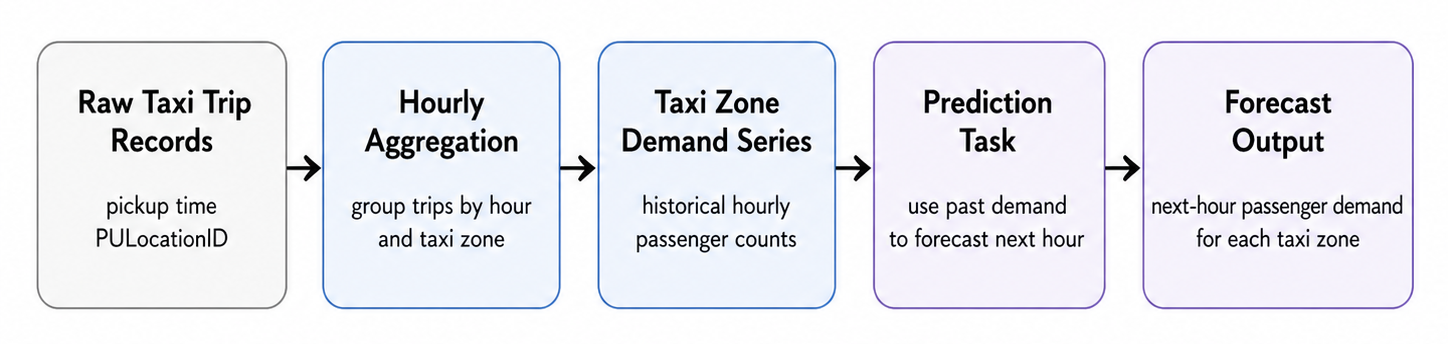
\includegraphics[width=1\textwidth]{img/1.1.png}
	\caption{Raw taxi trip records are first aggregated into hourly passenger counts for each taxi zone, forming zone-level historical demand series. Based on these time series, the forecasting task is to predict the passenger demand in the next hour for every taxi zone.}
	\label{fig:1.1}
\end{figure}

Multi-scale temporal modelling is a motivated candidate in this work. Urban taxi demand contains short-term fluctuations, daily repetition, weekly regularity, and slower trends. The implemented candidate uses four branches corresponding to 1-hour, 1-day, 1-week, and 1-month contexts, with LSTM, Transformer, and GRU components. This design tests the hypothesis that explicit temporal horizons provide complementary predictive information \cite{liao2022taxi,su2025transformer}. Chapter~5 evaluates that hypothesis directly and selects TCN, rather than multi-scale, for the causal residual experiments.



Equally important is the decision to adopt per-zone temporal training rather than a monolithic city-wide temporal model. The project uses the incremental multi-scale manager, allowing previously trained zone models to be updated as rolling windows advance. Experiments~2--6 reuse cached TCN forecasts and do not invoke the multi-scale manager. These are distinct temporal configurations rather than one universal rolling mode.

The uncertainty component further differentiates this framework from a standard temporal predictor. Monte Carlo Dropout generates repeated stochastic forward passes and estimates predictive variance \cite{gal2016dropout}. These estimates are combined with a historical-support prior and a historical-consistency score derived from 24-hour, 168-hour, and 720-hour demand summaries. The resulting confidence value is evaluated both as a graph node feature and as an optional residual-loss weight. It is interpreted as relative reliability rather than a calibrated probability of correctness.

The graph refinement stage addresses the main limitation of independent temporal forecasting: lack of spatial correction. After the base model generates per-zone next-hour predictions, the second stage treats these values as priors and learns residual corrections on a graph. The experiments consider geographic adjacency and rolling origin--destination flow graphs. GraphSAGE is not asked to predict demand from scratch. Instead, it learns how the initial temporal estimate should be adjusted once relational spatial context is taken into account \cite{hamilton2017graphsage}.

The comparison between origin--destination flow graphs and geographic adjacency is theoretically meaningful. A mobility system is shaped not only by physical proximity but also by functional interaction. Two zones may be geographically near yet weakly related in taxi demand, while distant zones can be strongly connected by travel flow. The graph ablation therefore tests whether rolling OD information provides an advantage over geographic structure under the same causal residual protocol \cite{xue_2020_spatialtemporal,ke2021od}.

The rolling evaluation protocol is another defining feature of this study. Instead of training once and reporting static test results, the pipeline advances target time step by time step, recalculating predictions and metrics at each hour. This setup better resembles how forecasting systems are used in deployment, where the model must repeatedly produce near-future estimates as new time points arrive. Rolling evaluation is important not only for realism but also for diagnosis. It reveals whether performance is stable over time, whether certain hours are systematically harder than others, and whether the spatial refinement stage consistently improves over the temporal baseline.

\section{Research Aim and Questions}

Against this background, the aim of this thesis is to investigate whether a causal two-stage architecture can improve hourly urban taxi demand forecasting by combining a temporal backbone, historical-residual graph refinement, and confidence-aware reliability analysis.

\begin{figure}[h]
	\centering
	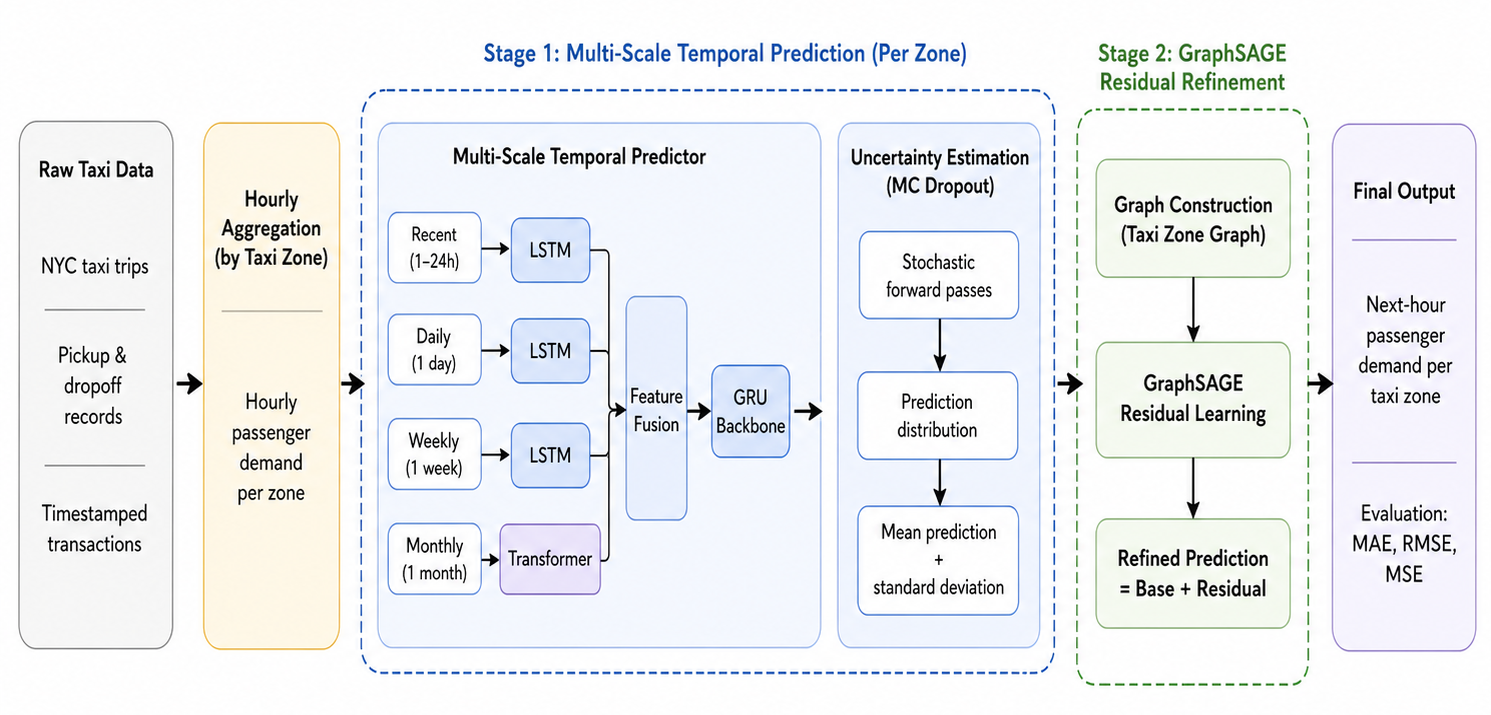
\includegraphics[width=1\textwidth]{img/1.2.png}
\caption{Framework for taxi-zone passenger demand prediction using a benchmarked temporal backbone and GraphSAGE-based residual refinement. The multi-scale architecture is one temporal candidate; TCN is selected for the causal residual experiments.}
	\label{fig:1.2}
\end{figure}

More specifically, this thesis addresses the following research questions:

\begin{enumerate}
	\item Which temporal backbone provides the strongest causal rolling baseline, and how does multi-scale compare with TCN under the same protocol?
	
	\item Does GraphSAGE-based residual refinement, trained only on earlier labelled snapshots, improve prediction accuracy compared with the temporal baseline?
	
	\item Do node features, graph topology, and confidence-derived weighting improve causal graph residual refinement, and does confidence reflect realised error?
	
	\item Are rolling OD graphs materially better than geographic graphs under the same causal residual protocol?
\end{enumerate}

\section{Contributions of This Thesis}

Accordingly, the main contributions of this work can be summarised as follows:

\begin{enumerate}
	\item It evaluates a broad causal temporal-backbone benchmark, including a matched twelve-window multi-scale run, and selects TCN as the slightly stronger backbone for the residual experiments.
	
	\item It introduces causal GraphSAGE residual refinement: residual supervision is drawn only from snapshots earlier than the target hour, while the target-hour graph is reserved for inference and evaluation.
	
	\item It evaluates confidence as both a node feature and an optional sample-weighting signal, using historical support, MC Dropout stability, and historical consistency, and directly tests its association with realised error.
	
	\item It compares no-graph, geographic, and causal rolling OD topologies and documents the scope limits of the resulting rolling evaluation.
\end{enumerate}

Together, these components form a practical and extensible foundation for urban demand forecasting in settings where temporal complexity, spatial coupling, and uncertainty must all be considered simultaneously.

\section{Thesis Structure}

The remainder of this thesis is organised as follows. Chapter~2 reviews related work on urban demand forecasting, multi-scale temporal sequence modelling, graph neural networks, and uncertainty-aware prediction. Chapter~3 formalises the problem setting and presents the proposed two-stage framework in detail, including temporal architecture, confidence construction, graph refinement, and rolling inference logic. Chapter~4 describes the implementation pipeline, data preparation process, key classes, and engineering decisions reflected in the codebase. Chapter~5 evaluates the temporal baseline and graph-refined model under rolling forecasting conditions and discusses performance patterns. Chapter~6 discusses the main findings, limitations, and future work. Finally, Chapter~7 concludes the thesis.
	
	\chapter{Literature Review}
\section{Introduction to the Literature Context}

Urban mobility forecasting has become a central problem in intelligent transportation systems because accurate short-term demand estimates influence vehicle dispatching, idle cruising reduction, passenger waiting time, congestion management, and the overall operational efficiency of city-scale transport services \cite{liu2022survey,khalesian2024area}. In large metropolitan areas, taxi demand is not only highly dynamic but also strongly heterogeneous across space and time \cite{qian_2015_spatial,tang2019spatiotemporal}. Different urban regions exhibit distinct activity rhythms shaped by commuting peaks, nightlife, commercial density, tourism, and residential land use \cite{tang2019spatiotemporal}. At the same time, the temporal behaviour of demand is rarely governed by a single periodic pattern. Instead, it reflects a mixture of short-term fluctuation, daily repetition, weekly regularity, and longer-range seasonal tendencies, which makes hourly taxi demand forecasting a difficult spatiotemporal learning task rather than a conventional univariate time-series regression problem \cite{jiang2022survey,liao2022taxi}.

The challenge becomes more pronounced when the forecasting objective is defined at the level of individual Taxi Zones. Fine-grained zone-level prediction is practically useful because dispatch systems, relocation strategies, and local service balancing all depend on geographically resolved demand estimation \cite{khalesian2024area,riley2020dispatch}. However, a disaggregated formulation also introduces additional statistical difficulty. Some zones generate abundant historical observations, while others are comparatively sparse or irregular. In low-activity regions, the observed series may contain many zero or near-zero counts interspersed with occasional surges, making the learning problem noisy and unstable \cite{zhuang2022sparse}. In high-activity districts, by contrast, the model must handle stronger amplitude variation and potentially sharper peak transitions, requiring effective modelling of complex spatial-temporal dependence \cite{wu2019graph,huang2022dstgnn}. A forecasting framework that performs well across all zones therefore needs to balance sensitivity to local temporal dynamics with robustness to data sparsity and uncertainty.

A second source of complexity lies in the spatially coupled nature of urban travel demand. Taxi zones do not evolve independently. Neighbouring regions, or regions connected by strong origin-destination flows, often exhibit correlated demand patterns because travel activity propagates through the city via commuting corridors, business districts, airports, entertainment clusters, and residential catchment areas \cite{xue2020spatiotemporal,ke2021od}. A purely per-zone temporal model can learn local history effectively, but it may fail to correct errors that arise when neighbouring zones move coherently or when a zone's local history is insufficient to explain its next-hour demand. This is particularly problematic under rolling forecasting conditions, where predictions must be refreshed hour by hour and small local errors can accumulate into spatially inconsistent outputs. Capturing such dependence therefore requires a representation that can use structural information beyond the isolated time series of a single region \cite{jiang2022survey}.

For this reason, recent research on traffic and mobility prediction has increasingly moved toward spatiotemporal architectures that combine temporal sequence modelling with graph-based spatial learning \cite{jiang2022survey,fu2024survey}. Temporal models such as recurrent neural networks and transformer variants are effective for extracting sequential dependencies, whereas graph neural networks offer a principled way to propagate information across related regions \cite{jiang2022survey}. Yet the integration of these components is not straightforward. End-to-end spatiotemporal models can be powerful, but they are often computationally heavy, difficult to interpret, and less flexible when the temporal and spatial signals differ in quality across nodes \cite{garcia2023explainability,liu2025review}. In practical city-scale forecasting, there is value in separating the problem into an initial temporal prediction stage and a subsequent spatial correction stage. Such a design allows the first component to focus on modelling zone-specific temporal regularity while the second component exploits graph structure to refine predictions in a controlled and interpretable manner \cite{shao2022d2stgnn}.

Another important issue is uncertainty. Most prediction systems output a single point estimate, but for urban demand forecasting this is frequently insufficient, since recent work has shown that spatiotemporal travel demand prediction benefits from explicitly quantifying predictive uncertainty rather than relying only on deterministic outputs \cite{zhuang2022sparse,wang2024probgnn}. Prediction reliability varies significantly across time and across regions. A confident prediction in a historically dense, stable zone should not be treated in the same way as a volatile estimate produced for a sparse zone with weak historical support \cite{zhuang2022sparse}. If uncertainty can be quantified explicitly, it can guide later stages of the model and reduce the influence of unreliable nodes during learning. Therefore, uncertainty is not merely an auxiliary diagnostic quantity; it can also serve as a useful signal for weighting, calibration, and robustness enhancement.

The present project is motivated by precisely these difficulties. It addresses hourly taxi demand prediction for New York City Taxi Zones through a two-stage, confidence-weighted, multi-scale forecasting framework. The system is organised around three linked ideas: first, each zone is predicted with an incrementally updated multi-branch temporal model that captures information at hourly, daily, weekly, and monthly scales; second, predictive uncertainty is estimated through Monte Carlo Dropout and fused with other reliability indicators to form a confidence score \cite{gal2016dropout}; third, the initial predictions are refined on a graph built from origin-destination flow relationships using a GraphSAGE residual learning module \cite{hamilton2017graphsage}. The overall pipeline is executed in a rolling fashion, producing hour-by-hour forecasts, metrics, and output files that simulate a realistic operational deployment setting.

This chapter therefore reviews the literature in six connected parts. First, it examines traditional approaches to urban demand forecasting and their limitations. Second, it reviews deep temporal sequence models and explains why multi-scale learning became important. Third, it surveys spatial modelling approaches, especially graph neural networks, and discusses the relevance of GraphSAGE-style aggregation. Fourth, it considers hybrid spatiotemporal architectures and the distinction between end-to-end fusion and two-stage refinement. Fifth, it reviews uncertainty estimation and confidence-aware learning. Finally, it discusses rolling forecasting and incremental adaptation, which are central to practical deployment. Throughout the chapter, the review will relate prior work back to the needs of the current project and identify the methodological gaps that the thesis should address.

\section{Traditional Urban Demand Forecasting Methods}

The earliest literature on transportation demand forecasting was dominated by statistical and econometric models. 

\begin{figure}[h]
	\centering
	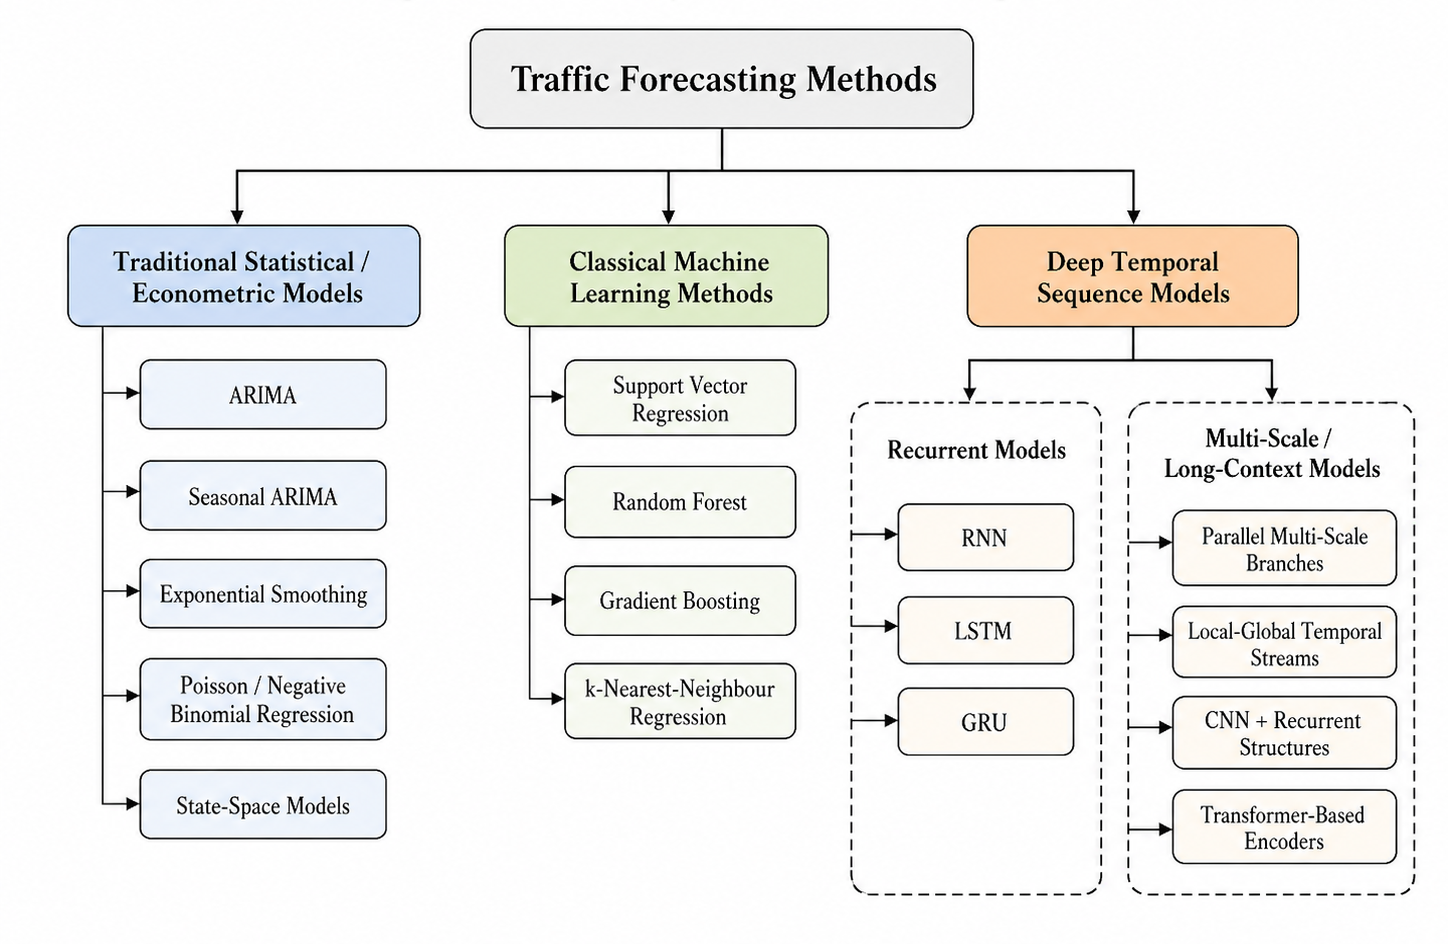
\includegraphics[width=1\textwidth]{img/2.1.png}
	\caption{Overview of representative traffic forecasting approaches, including traditional statistical models, classical machine learning methods, and deep temporal sequence models, with the latter further divided into recurrent and multi-scale or long-context architectures.}
	\label{fig:2.1}
\end{figure}


Classical methods included autoregressive integrated moving average models, seasonal ARIMA variants, exponential smoothing, Poisson and negative binomial regression, and state-space formulations \cite{petropoulos2020forecasting,lyu2021bigdata}. These methods remain attractive because they are interpretable, computationally light, and theoretically well understood. In settings with stable seasonality and relatively smooth temporal structure, such models can provide strong baselines. For aggregate traffic or passenger series, they often perform reasonably well when the forecasting horizon is short and the signal is dominated by linear dependence \cite{petropoulos2020forecasting}.

However, taxi demand forecasting at the zone level quickly exposes the limits of such models. First, linear autoregressive methods assume relatively simple dependence structures and struggle when multiple temporal scales interact nonlinearly. Second, they are poorly suited to sparse or highly intermittent zones where many observations are zero or near-zero \cite{zhuang2022sparse}. Third, classical models generally treat each spatial unit independently unless augmented with hand-designed exogenous terms or multivariate extensions, which become difficult to scale in city-wide settings \cite{jiang2022survey,safikhani2017nyc}. Fourth, the assumptions required for stationarity, residual independence, or parametric count structure are often violated by urban mobility data \cite{lyu2021bigdata}. These weaknesses motivated the field to adopt machine learning methods capable of handling high-dimensional nonlinearity more flexibly.

Before deep learning became dominant, methods such as support vector regression, random forests, gradient boosting, and k-nearest-neighbour regression were frequently applied to transport prediction \cite{medina2022review,roy2025transferability}. These models could capture nonlinear feature interactions better than traditional statistical methods, especially when provided with engineered inputs such as hour-of-day, day-of-week, weather indicators, holiday flags, and lagged demand values \cite{roy2025transferability,lyu2021bigdata}. Nevertheless, they still depended heavily on feature engineering and did not solve the core representation problem of spatiotemporal dependence. A random forest may capture nonlinear interactions among static covariates, but it does not naturally model long temporal memory or structured spatial propagation. Similarly, support vector methods can be effective on carefully prepared datasets but do not scale elegantly to multi-zone dynamic graphs with rolling re-estimation requirements \cite{jiang2022survey,medina2022review}.

A further limitation of both statistical and early machine learning approaches is that they often produce point forecasts without any integrated uncertainty mechanism. In urban mobility applications, this is a significant gap. Demand variance is not homogeneous across zones or time periods, and decision systems can benefit greatly from knowing which predictions are stable and which are unreliable \cite{zhuang2022sparse,wang2024probgnn}. Thus, even before discussing deep learning, the literature already points toward three essential requirements that simpler approaches do not jointly satisfy: nonlinear multi-scale temporal modelling, explicit spatial coupling, and reliability awareness \cite{jiang2022survey,zhuang2022sparse}.

These limitations are directly relevant to the current project. The system is designed around zone-level demand prediction with mixed short- and long-term temporal patterns, OD-related spatial coupling, and uncertainty-aware graph refinement through confidence scores. This implies that purely statistical baselines, while still necessary for comparison, cannot be the final methodological destination of the thesis. Instead, they serve mainly as conceptual stepping stones illustrating why a deeper spatiotemporal architecture is justified.

\section{Deep Temporal Sequence Models for Demand Forecasting}

The deep learning literature on forecasting introduced a major shift by replacing manual feature engineering with learned representations. Recurrent neural networks became especially influential because they provide a natural mechanism for modelling sequential dependence. Standard RNNs can, in principle, use previous hidden states to summarise temporal context, but in practice they suffer from vanishing and exploding gradient problems when sequences are long \cite{pascanu2013rnn}. This limitation led to the widespread adoption of Long Short-Term Memory networks and Gated Recurrent Units, both of which use gating mechanisms to regulate information flow and preserve relevant historical context over longer horizons \cite{hochreiter1997lstm,cho2014gru}.

\begin{figure}[h]
	\centering
	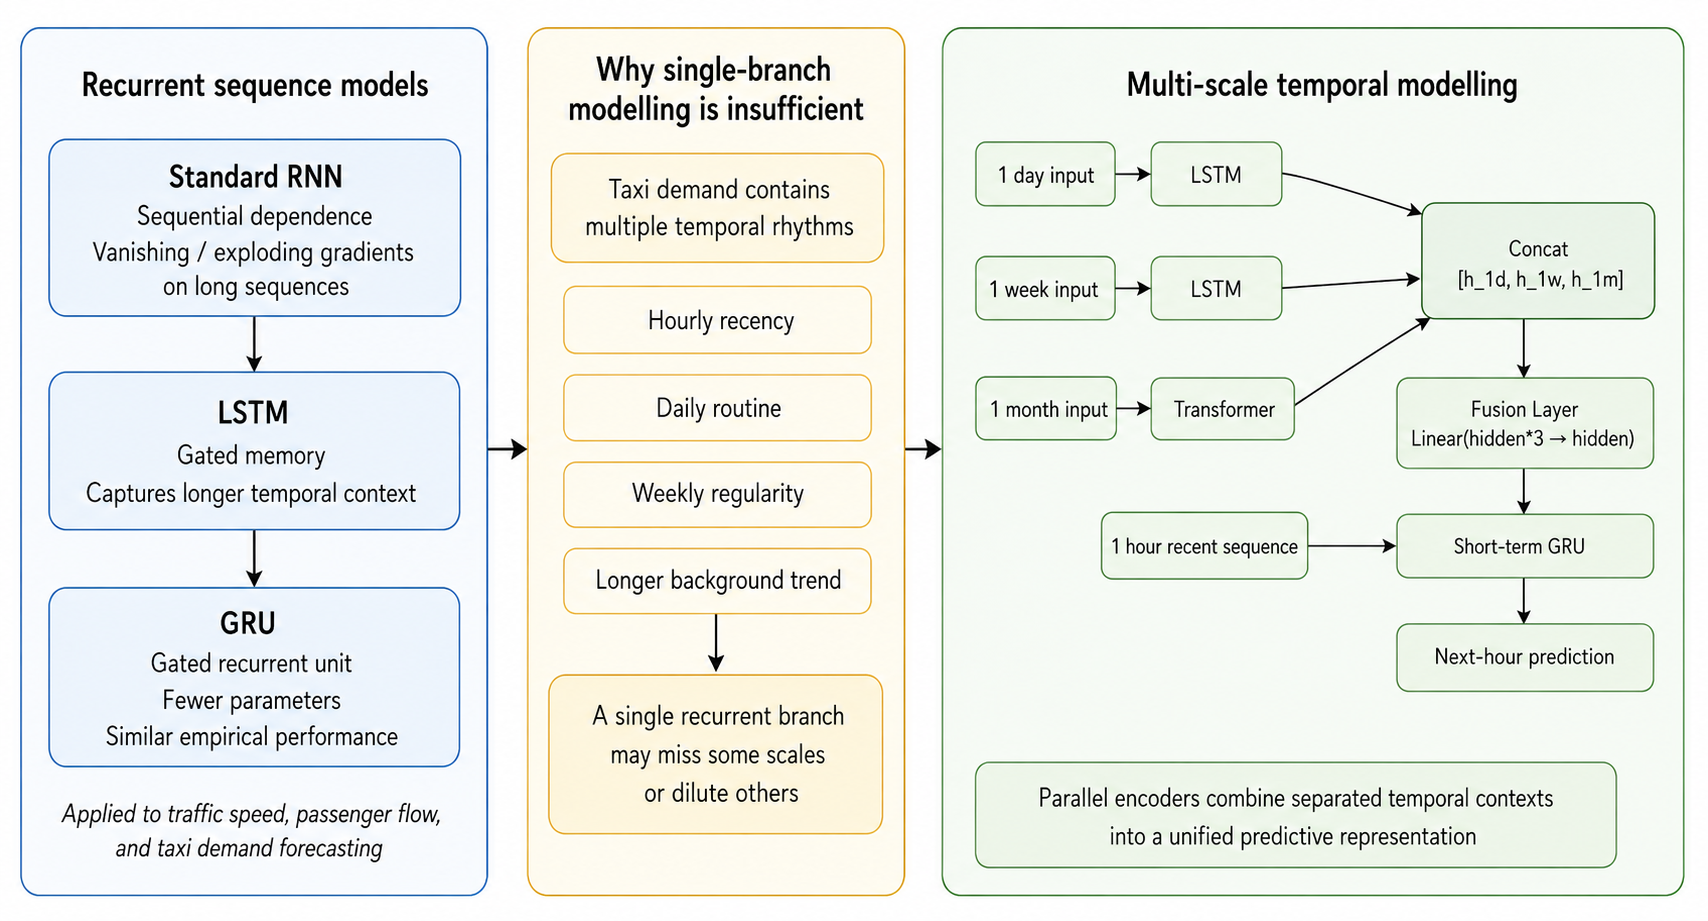
\includegraphics[width=1\textwidth]{img/2.2.png}
	\caption{Recurrent and multi-scale temporal modelling for demand forecasting.}
	\label{fig:2.2}
\end{figure}


In transportation forecasting, LSTM-based models were soon applied to traffic speed, passenger flow, and taxi demand because they captured nonlinear temporal dependence more effectively than traditional autoregressive models \cite{jiang2022survey,lstmtraffic2024survey}. GRUs offered a lighter-weight alternative with fewer parameters and often similar empirical performance \cite{chung2014gru}. In urban demand settings, recurrent models are useful because they can absorb sequential fluctuations without requiring explicit manual design of every lag interaction. They also adapt relatively naturally to rolling one-step-ahead prediction tasks, which is important for hourly operational forecasting.

Yet the recurrent literature also exposed a key problem: a single recurrent branch is often insufficient to capture the coexistence of multiple temporal rhythms. Taxi demand does not evolve only according to the immediately preceding hour. There are within-day cycles, weekly regularities, event-driven deviations, and slower baseline shifts. A model trained only on a short recent history may miss recurrent weekly effects; a model trained on a very long history may dilute immediate local momentum. This tension drove the literature toward multi-scale or multi-resolution temporal modelling \cite{liao2022taxi,effective2021multiresolution}.

Multi-scale temporal models attempt to process different context windows separately and then combine them into a unified predictive representation. Some methods use parallel recurrent branches fed with different lag lengths. Others separate local and global temporal streams, or introduce convolutional structures to summarise short-term patterns before recurrent integration \cite{effective2021multiresolution,kim2025dltimeseries}. More recently, transformer-based encoders have been used to model long-range dependencies, since attention mechanisms can relate distant time points more directly than purely recurrent hidden-state propagation \cite{zhao2026transformers,kim2025dltimeseries}. In mobility prediction, multi-scale designs are attractive because they align closely with known human activity rhythms: hourly recency, daily routine, weekly schedule, and longer background trend \cite{liao2022taxi,tang2019spatiotemporal}.

The current project follows this line of development quite explicitly. The temporal stage uses four scales: 1 hour, 1 day, 1 week, and 1 month. The implementation combines LSTM encoders for daily and weekly sequences, a Transformer-based pathway for the monthly context, and a GRU-centred output structure for short-term prediction. This makes the model neither a pure LSTM, pure GRU, nor pure Transformer architecture. Instead, it is a composite multi-branch design in which each component handles the timescale for which it is most suitable. Such a design is well supported by the literature because it reflects the widely recognised principle that no single temporal mechanism dominates all forecasting horizons equally \cite{kim2025dltimeseries,zhao2026transformers}.

Another relevant theme in the sequence-model literature is the trade-off between local adaptation and global sharing. Many deep forecasting studies train a single city-wide model using all zones jointly, often with embeddings to represent region identity. This can improve data efficiency because parameters are shared across zones. However, shared models may also obscure strong local heterogeneity, especially when different regions exhibit substantially different temporal patterns \cite{lim2021survey,sonnleitner2025heterogeneity}. A highly active commercial district and a low-density peripheral zone may not benefit equally from identical temporal parameters. By contrast, per-zone models allow local dynamics to be learned independently but can suffer from limited data in sparse regions. The project adopts a per-zone temporal modelling approach that preserves local structure while later compensating for spatial dependence through graph refinement. This choice aligns with literature that emphasises the importance of respecting regional heterogeneity in mobility prediction, but it also invites comparison with shared or meta-learned temporal models as possible future improvements \cite{liu2022ridesourcing,zheng2024fairness}.

A further issue concerns input scaling and zero inflation. Mobility count series often contain sharp spikes, long low-activity periods, and substantial imbalance across zones. In such settings, deep temporal models can become sensitive to amplitude disparities unless scaling is carefully handled. The framework uses MinMax scaling and dense hourly reconstruction with missing hours filled by zero. These are practical engineering decisions consistent with the broader forecasting literature, though they also introduce open questions. For example, MinMax scaling can be sensitive to extreme values, and zero-filling may blur the distinction between true absence and missing observation. These issues do not invalidate the approach, but they are the kinds of modelling assumptions that literature review should surface because they shape how results ought to be interpreted \cite{zhuang2022sparse,lim2021survey}.

Overall, the literature on deep sequence learning provides strong support for the project's temporal stage. It justifies the movement beyond classical time-series baselines, motivates the use of gated recurrent models, and explains the need for explicitly multi-scale architecture \cite{lim2021survey,kim2025dltimeseries}. At the same time, it suggests several comparative angles that the thesis could later exploit: single-scale versus multi-scale models, GRU-only versus hybrid designs, shared city-level versus per-zone models, and recurrent versus transformer-heavy long-context encoders.

\section{Multi-Scale Modelling as a Distinct Research Theme}

Although multi-scale sequence learning can be discussed under deep temporal modelling, it has become important enough in transportation prediction to warrant a separate treatment. The broader forecasting literature repeatedly shows that urban mobility contains superposed rhythms rather than one dominant cycle. Commuting activity imposes strong diurnal repetition, weekends introduce behavioural discontinuity, and slower structural shifts emerge from tourism, economic conditions, school terms, and seasonal patterns. Models that use only a fixed-length lag often end up overfitting one scale and under-representing another \cite{tang2019spatiotemporal,liao2022taxi}.

One family of multi-scale approaches uses handcrafted lag groups. For instance, a model may include the last few hours, the same hour from the previous day, and the same hour from the previous week as separate feature channels. This strategy is simple and often effective, but it depends on fixed assumptions about what temporal anchors matter most. A more flexible family of approaches learns these temporal scales directly using parallel encoders, hierarchical recurrent modules, dilated convolutions, or attention over multiple resolution levels. The key insight is that temporal scale is not just an engineering hyperparameter; it is a structural property of the forecasting problem \cite{huang2021multiresolution,lim2021survey}.

For taxi demand in particular, multi-scale methods are especially appropriate because the service is highly responsive to recurring human routines. The same district can behave very differently on weekday mornings, Friday evenings, weekends, and holiday periods. Moreover, the intensity of these patterns may vary across zones. A business district may show strong daily periodicity, while an airport may show broader multi-day or weekly variation linked to travel patterns. This means a robust model should not assume that all temporal information is equally informative for all nodes at all times \cite{tang2019spatiotemporal,liao2022taxi}.

The project's four-scale design can be understood in this literature context as a pragmatic but theoretically coherent decomposition. The hourly branch preserves immediate recency. The daily branch captures within-day repetition and typical local rhythm. The weekly branch addresses weekday--weekend structure and broader behavioural recurrence. The monthly branch serves as a long-range trend context that can stabilise the model against short-lived noise. The literature does not prescribe exactly these four windows as universally optimal, but it strongly supports the principle behind them: short-term prediction becomes more reliable when informed by explicitly separated temporal contexts \cite{liao2022taxi,huang2021multiresolution,lim2021survey}.

Another benefit highlighted by the multi-scale literature is interpretability. When a model is organised by time horizon, it becomes easier to reason about what kind of information is driving the forecast. This is especially useful in research-oriented forecasting systems, where one often wants to know whether gains come from local recency, medium-range seasonality, or longer historical context. The framework also uses stochastic sampling of branch behaviour through MC Dropout to estimate predictive uncertainty \cite{gal2016dropout}. This means the project not only separates temporal scales structurally but also measures their stochastic behaviour. From a literature perspective, this is an interesting bridge between multi-scale representation learning and uncertainty analysis.

At the same time, multi-scale models introduce extra design complexity. The more branches one uses, the more important fusion becomes. A poorly designed fusion layer can negate the benefits of separate temporal encoding by collapsing incompatible information too aggressively. The literature offers several fusion strategies, including concatenation followed by projection, gating, attention-based weighting, and hierarchical fusion mechanisms \cite{lim2021survey,lim2021tft,ling2024msrgcn}. The project currently uses linear fusion before the GRU-based output stage. This is a reasonable baseline choice, but the literature suggests that learnable cross-scale attention or adaptive gating could be explored later as a more expressive alternative \cite{lim2021tft,ling2024msrgcn}.

\section{Spatial Dependence Beyond Geography}

A recurring lesson in transportation literature is that ``space'' should not be reduced to Euclidean closeness. Two zones may border each other yet function quite differently, while zones farther apart may be tightly linked through mobility behaviour. This is especially true in taxi systems, where trip patterns often follow business corridors, airport routes, nightlife clusters, and commuting flows rather than simple neighbourhood adjacency \cite{jiang2022survey,Rong_2024}. As a result, graph construction itself becomes a research question.



The most basic graph uses shared physical borders. This is easy to build and intuitively interpretable, but it can be too coarse. Distance-based graphs soften the binary decision by weighting nodes according to geographical separation. These are useful when movement likelihood decays smoothly with distance, but they still fail to capture directed or asymmetric travel relationships. Mobility-flow graphs improve on this by using actual trip movement between regions. Such graphs can encode strong functional dependence even when geography alone would not. Similarity graphs go one step further, linking zones with correlated historical behaviour or comparable temporal signatures \cite{ke2021od,jiang2022survey}.

The present project chooses an origin-destination flow matrix as the basis for graph construction. In literature terms, this is a strong choice because it ties the graph to actual travel interaction. The system maps zones through a lookup table and constructs adjacency when flow weight is positive. This means the graph is operationally grounded in the data-generating process, not merely overlaid as a generic structure. For a taxi-demand problem, this is more meaningful than an arbitrary lattice or shapefile-only adjacency \cite{ke2021od}.

However, literature also makes clear that graph construction and graph usage should be aligned. If edge weights quantify flow intensity, message passing should distinguish stronger and weaker edges rather than treating all connections as equivalent \cite{jiang2022survey,west2025weighted}. The reported graph study instead treats geographic and OD relations as alternative topology controls under mean GraphSAGE aggregation. Remaining questions concern the use of edge-weight definitions, dynamic reweighting based on time or confidence, and joint learning of relation strength \cite{jiang2022survey,timegnn2023,dgcntraffic2020}.

The literature on dynamic graphs is also relevant here. Urban mobility relationships are not constant over time. Morning commute patterns differ from evening leisure travel; weekday relations differ from weekend relations. A static OD graph captures average structure but not temporal variation in connection strength. This does not mean the current static graph is wrong, but it does mean that the thesis should frame it as an approximation. Dynamic graph models, time-conditioned edge weights, or multi-graph ensembles could later provide richer spatial realism \cite{dynamicgnnsurvey2024,dgcntraffic2020,timegnn2023}.
\section{Graph Neural Networks for Transportation Forecasting}

Graph neural networks became central in transportation forecasting because they allow node representations to be updated through learned neighbourhood aggregation. In road traffic, the intuition is straightforward: nearby sensors influence one another through network flow. In taxi demand forecasting, the same principle applies more abstractly at the zone level: regions linked through travel behaviour or proximity may share demand dynamics or error structure. GNNs convert this intuition into learnable operators.


\begin{figure}[h]
	\centering
	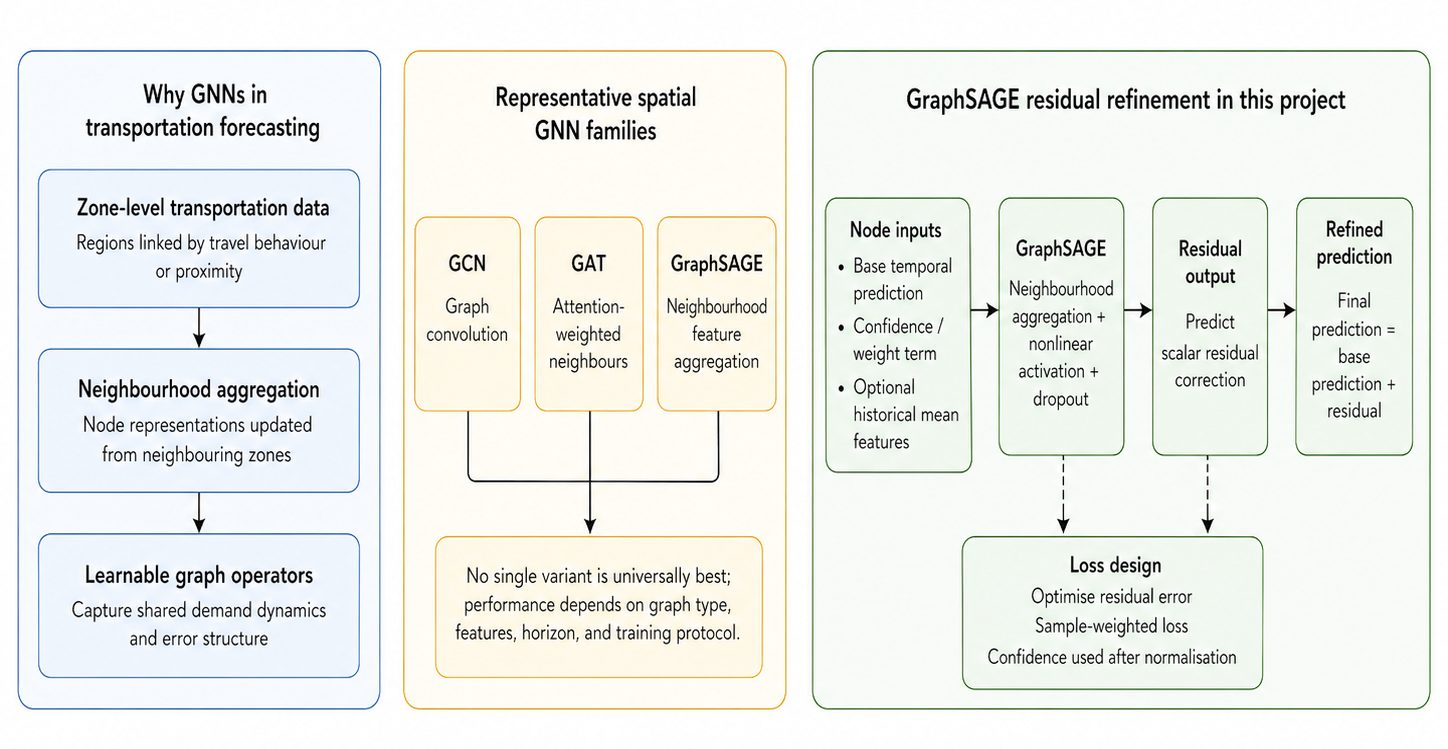
\includegraphics[width=1\textwidth]{img/2.3.png}
	\caption{GraphSAGE-based refinement uses neighbourhood aggregation on the taxi-zone graph to learn residual corrections from base predictions, confidence weights, and optional historical features, producing a refined forecast for each zone.}
	\label{fig:2.3}
\end{figure}

Early graph convolutional methods generally relied on spectral formulations or fixed graph filters. Later spatial GNNs, including Graph Convolutional Networks, Graph Attention Networks, and GraphSAGE, shifted focus toward more flexible neighbourhood aggregation. Graph Attention Networks learn to weight neighbours through attention coefficients. GraphSAGE learns how to aggregate neighbourhood features and is often favoured for scalability and inductive behaviour. In transportation literature, no single GNN variant is universally best; performance depends heavily on graph type, feature design, horizon, and training protocol.

The current project's use of GraphSAGE is methodologically sensible because the graph stage receives heterogeneous node features rather than raw graph signals alone. Node inputs include the base temporal prediction, a confidence or weight term, and optionally historical mean features. The task is then to infer a residual correction. This is a good fit for GraphSAGE because the model can aggregate neighbour attributes and infer how the local node should be adjusted relative to its relational context. The graph model is lightweight, uses neighbourhood aggregation, nonlinear activation, dropout, and predicts a scalar residual that is added back to the base prediction. This places the model within a well-established class of graph refinement architectures.

The loss design is also noteworthy. Rather than minimising absolute prediction error directly on raw demand, the graph model optimises residual error with sample weighting. If confidence is provided, node losses are weighted accordingly after normalisation. This is an elegant compromise between full graph forecasting and purely heuristic smoothing. It allows the temporal model to carry most of the predictive burden while the graph stage focuses on structured correction where it is most reliable.

Still, the GNN literature suggests several comparisons that would strengthen the thesis. First, GraphSAGE should ideally be compared with at least one alternative such as GCN or GAT. Second, If edge weights encode flow intensity, message passing should ideally be sensitive to differences in edge strength rather than collapsing all connected pairs into a uniform neighbourhood relation. Third, graph depth should be controlled to avoid over-smoothing, especially since Taxi Zones may vary sharply even among neighbours. Fourth, the graph objective should be evaluated under a temporally valid protocol to demonstrate actual forecast refinement rather than same-snapshot fitting. These issues do not undermine the current choice of GraphSAGE, but they define the standards against which its use should be discussed in the literature review and later experiments.

\section{Two-Stage Residual Refinement Versus End-to-End Spatiotemporal Learning}

One of the most important conceptual distinctions in the literature is whether spatial and temporal modelling should be tightly intertwined or sequentially decomposed. End-to-end spatiotemporal models often dominate benchmark leaderboards because they jointly optimise all components. However, these models also make it harder to identify what each part contributes. If performance improves, is it because temporal encoding became better, because spatial propagation worked well, or because one compensates for another in a way that is hard to interpret \cite{jiang2022survey,garcia2023explainability}?

Residual two-stage refinement offers a different philosophy. Instead of trying to learn everything simultaneously, it first obtains a competent temporal forecast and then learns structured corrections. This approach is common in calibration, post-processing, and boosting-style systems, even if it is less fashionable in some deep-learning benchmark literature. Its strength lies in modularity and interpretability. If the graph stage improves performance, one can directly measure the incremental value of spatial correction. If it fails, the base temporal model remains intact \cite{shao2022d2stgnn}.

The present project clearly adopts this residual view. The graph refinement stage treats the temporal prediction as a prior and learns residual adjustment. This is theoretically attractive because taxi demand is already strongly predictable from local temporal history; the graph stage need not rediscover that structure from scratch. Instead, it can focus on neighbourhood-based consistency and cross-zone correction. In practice, this also reduces the burden on the graph model because residuals are often smoother and lower-variance than raw targets.

From a literature perspective, residual refinement also provides a natural bridge to ensemble thinking. The temporal model and graph model can be seen as experts with different strengths: one captures intra-zone temporal recurrence, the other captures inter-zone relational adjustment. Their combination is not a crude average but an ordered composition in which the graph stage edits the temporal output. This is more principled than simple ensembling and more interpretable than monolithic end-to-end fusion \cite{garcia2023explainability,shao2022d2stgnn}.

The main methodological challenge, again, is evaluation. Residual refinement must be assessed under conditions that match true forecasting. If the graph stage is trained on the same nodes and same hour that it later ``improves,'' then what is being measured may be correction fit rather than predictive generalisation. The literature is clear that temporal ordering matters in forecasting evaluation, and rolling-origin or prequential evaluation is generally preferred to leakage-prone estimation setups \cite{hewamalage2022pitfalls,cerqueira2020evaluating}. Accordingly, the reported experiments train the graph stage on residual snapshots earlier than the target hour and reserve that hour for inference and evaluation. Resetting histories within each 24-hour window and the absence of a temporally disjoint hold-out cohort still limit the strength of the generalisation claim.

\section{Historical Summary Features and Lightweight Context Injection}

A subtle but useful idea in forecasting literature is that a downstream model does not always need access to full raw sequences if it can receive carefully chosen summary statistics. This matters because graph models are often simpler than temporal models and may become expensive if full temporal sequences are attached to every node. Historical summary features provide a compromise: they inject context compactly \cite{jiang2022survey,lim2021survey}.

The graph stage can receive mean demand over the previous 24 hours, 168 hours, and 720 hours. These features encode short-, medium-, and longer-term demand level without forcing the graph network to process complete time series. In literature terms, this is a form of context distillation. The temporal stage extracts rich sequential information; the graph stage then receives both the base prediction and compressed historical indicators that help judge whether a correction is plausible \cite{lyu2021bigdata,demandfeatures2023}.

Such features are especially useful when base predictions are noisy. Suppose two zones have the same predicted next-hour demand, but one has a high recent mean and the other has been mostly inactive. A graph model receiving recent average features can treat those cases differently. Historical features also typically require stabilisation before graph use, especially for skewed count distributions, and transformations such as logarithmic compression are well supported by the literature \cite{akram2023counts,lyu2021bigdata}.

The literature suggests that this design could be expanded. Instead of only simple means, one could include recent variance, trend slope, same-hour-last-week value, holiday flags, or uncertainty summaries. However, there is also virtue in parsimony. The current design keeps graph features compact and interpretable, which is appropriate for a first thesis implementation. This makes historical summary features a lightweight but theoretically grounded mechanism deserving empirical validation through ablation.

\section{Confidence Fusion as an Emerging Research Direction}

The notion of confidence fusion deserves special attention because it is one of the most distinctive aspects of the project. Confidence is not derived from one metric alone. Instead, it combines three components: a prior score $p_i$ based on the historical data richness of zone $i$, a stability score $s_i$ derived from the predictive variance estimated by Monte Carlo Dropout, and a historical-consistency score $h_i$ computed from the agreement among 24-hour, 168-hour, and 720-hour demand summaries. These components are merged through a weighted logarithmic combination to produce the final confidence score $c_i$:
\[
\log c_i = w_p \log p_i + w_s \log s_i + w_h \log h_i,
\]
where $w_p$, $w_s$, and $w_h$ are the fusion weights assigned to the prior, stability, and historical-consistency components, respectively. Equivalently, this can be written as
\[
c_i = \exp\!\left(w_p \log p_i + w_s \log s_i + w_h \log h_i\right).
\]
The fixed confidence baseline uses equal component weights, $w_p = w_s = w_h = 0.33$ \cite{gal2016dropout,zhuang2022sparse}.

\begin{figure}[h]
	\centering
	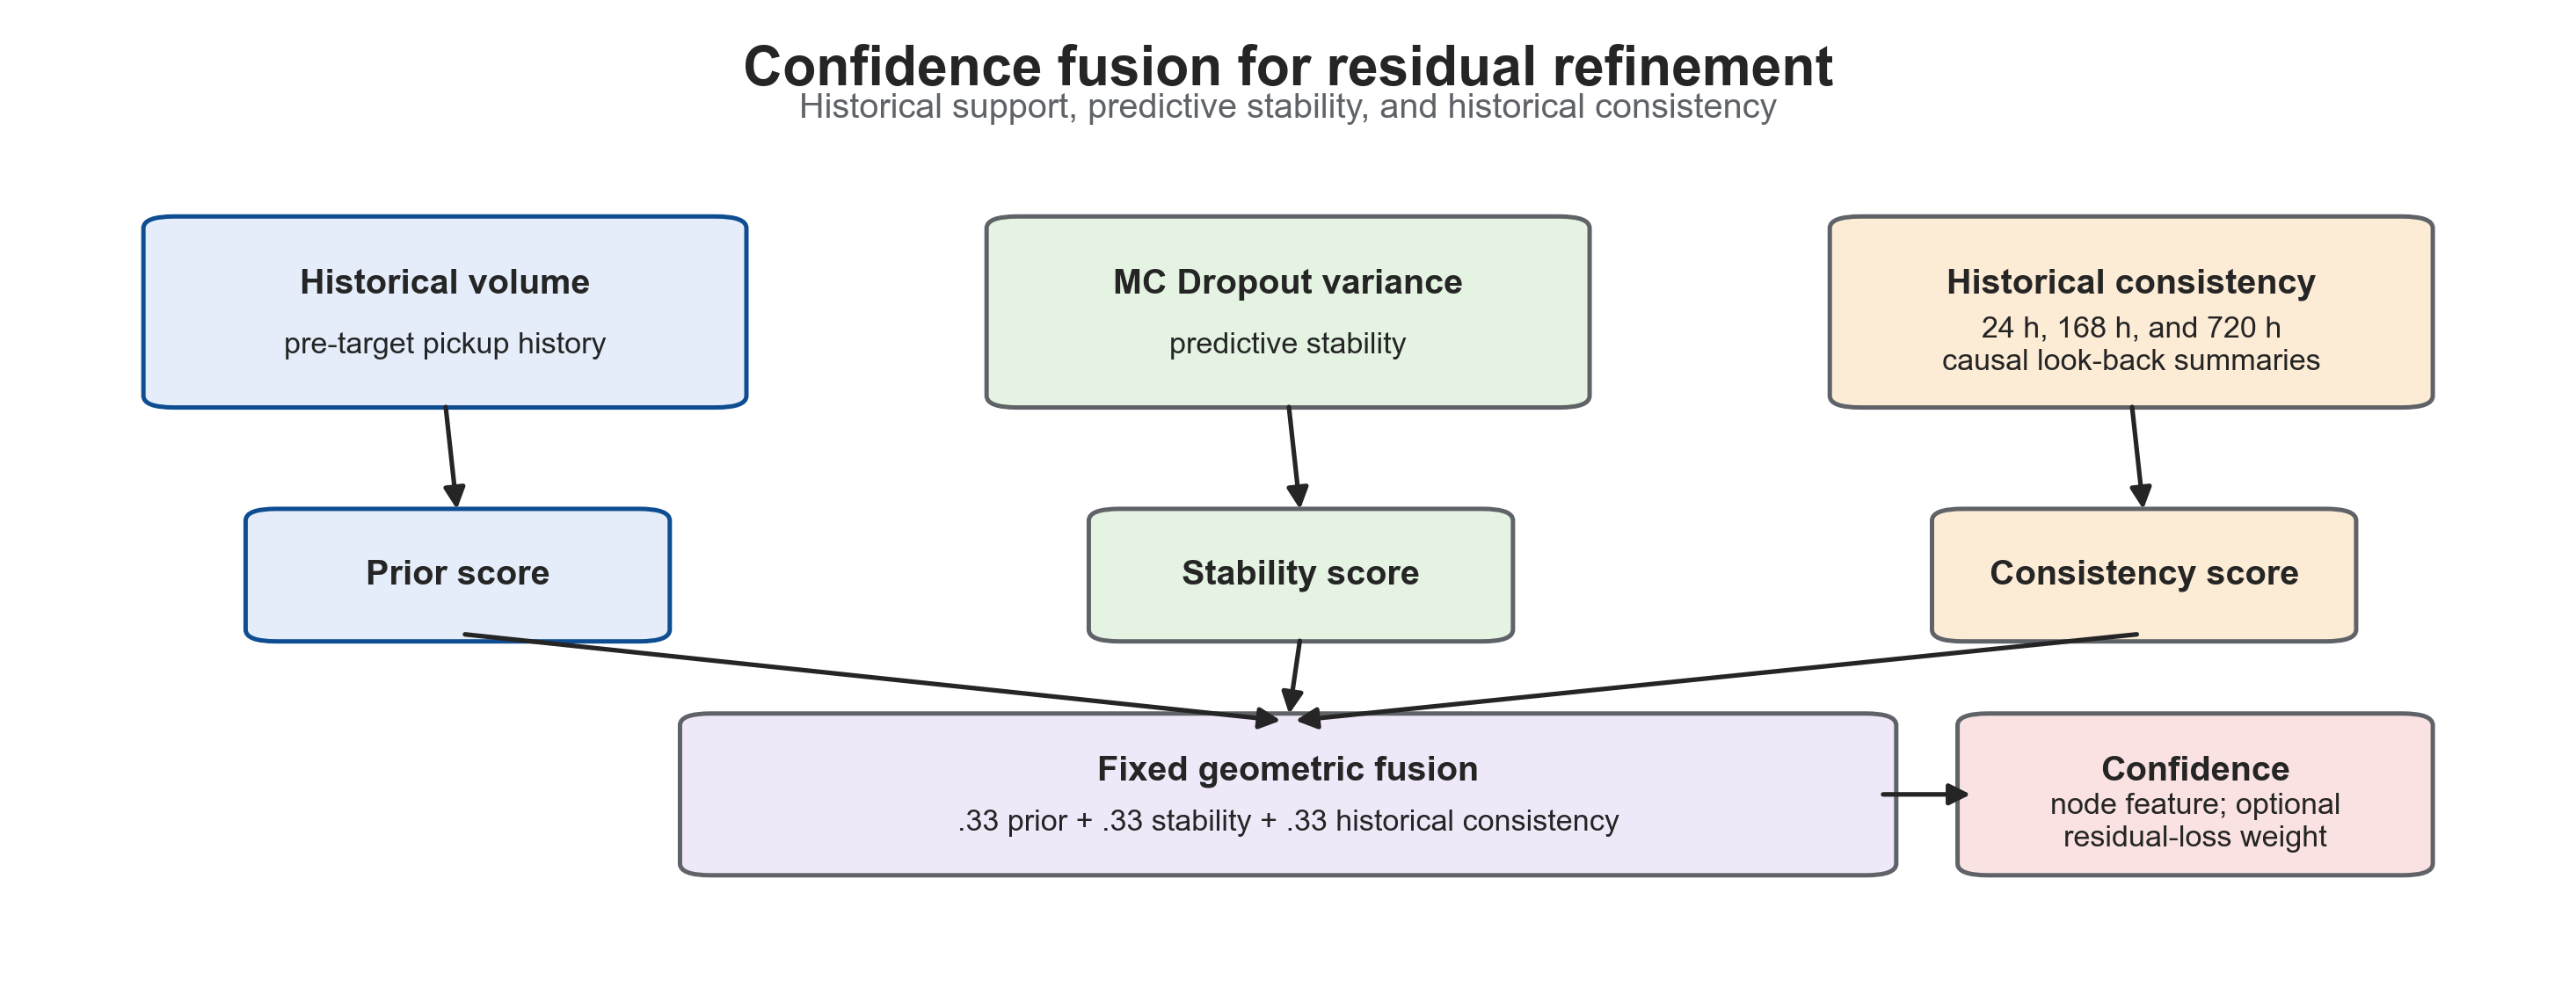
\includegraphics[width=1\textwidth]{img/2.4.png}
\caption{Confidence fusion integrates prior score, stability score, and historical consistency into a final confidence score for confidence-aware graph refinement.}
	\label{fig:2.4}
\end{figure}


This design is interesting in relation to literature because it blends three complementary signals. Historical sufficiency reflects how much evidence the model has seen for a zone. Stability reflects the model's internal consistency under stochastic perturbation. Historical consistency reflects agreement between short-, medium-, and longer-term demand levels. The resulting score is used as a node feature and, in selected ablations, as a residual-loss weight \cite{wang2024probgnn,park2022confidenceaware}.

At the same time, literature invites a critical discussion of how such fusion should be justified. The experiments compare fixed, searched, and learned fusion weights, rather than assuming that one fixed setting transfers across cities, datasets, or time horizons. A Bayesian calibration layer and repeated weight-selection trials remain useful future extensions \cite{wang2024gnnuncertaintysurvey,moon2020confidence}.

Another open question is whether confidence should be static per prediction or interactive during message passing. Current use is primarily through loss weighting, but literature suggests richer possibilities: confidence could scale outgoing messages, reweight edges, gate attention, or decide whether a node should rely more on local versus neighbour information. These extensions would move the system closer to fully confidence-aware graph learning \cite{park2022confidenceaware,chernikova2025uncertaintympnn}.

\section{Uncertainty Estimation and Robust Forecasting}

Uncertainty estimation has become increasingly important in applied machine learning because prediction error alone does not reveal confidence. In forecasting, uncertainty can arise from noise in the data, sparsity of observations, model misspecification, limited training coverage, and genuine unpredictability in the underlying process \cite{gal2016dropout,wang2024gnnuncertaintysurvey}. For urban taxi demand, these issues are especially significant because demand variability differs dramatically across zones and across hours \cite{zhuang2022sparse,wang2024probgnn}. A quiet residential zone at 3 a.m. and a business district at 8 a.m. pose different uncertainty profiles, even if their average counts are similar over some period.

The uncertainty literature commonly distinguishes several forms of uncertainty. Aleatoric uncertainty reflects irreducible data noise, while epistemic uncertainty reflects uncertainty in model parameters or structure due to limited knowledge. In practice, deep forecasting systems often use approximations to obtain at least a useful proxy for uncertainty. Monte Carlo Dropout is one of the most widely used such methods. By keeping dropout active at inference time and performing repeated stochastic forward passes, one obtains a distribution of predictions whose mean and variance can be used as approximate measures of uncertainty. This approach is attractive because it is simple to implement, computationally manageable, and easily integrated into existing deep models \cite{gal2016dropout}.

The project directly adopts this strategy. Repeated stochastic sampling in the temporal model yields a predictive mean and standard deviation, and branch-level stochastic behaviour can also be analysed across temporal scales. Literature supports this use of MC Dropout as a pragmatic method for uncertainty-aware forecasting, especially when the objective is not full Bayesian inference but operational reliability assessment \cite{gal2016dropout,zhuang2022sparse}.

What makes the current project more interesting is that uncertainty is not used in isolation. It is fused with historical sufficiency and historical consistency. Historical sufficiency acts as a prior, rewarding zones with richer observation history. Historical consistency captures agreement across three causal look-back summaries. This confidence fusion is evaluated as both a node feature and a residual-loss weight, moving the framework from passive uncertainty reporting to active confidence-aware modelling \cite{wang2024gnnuncertaintysurvey}.

There are, however, several literature-based questions that this design raises. First, is the confidence score well calibrated? MC Dropout variance is useful, but it is not guaranteed to match true predictive reliability without calibration analysis \cite{gal2016dropout,uncertaintygnnsurvey2025}. Second, do the three components require repeated validation across temporal and geographic settings? Third, can confidence be used more directly in message passing or feature gating, rather than only as a node feature and loss weight? These questions situate the project as a practical design rather than a final uncertainty solution \cite{wang2024gnnuncertaintysurvey,hu2025uncertaintygnn}.

Another relevant strand of literature concerns robust learning under noisy or sparse supervision. Confidence-aware weighting resembles ideas from curriculum learning, self-paced learning, heteroscedastic regression, and sample reweighting. The common principle is that not all observations should contribute equally to optimisation \cite{ren2018reweight,shi2023selfpaced}. In the context of graph refinement, this is especially valuable because a bad node can influence not only its own error term but also the neighbourhood information used by others. Weighting the graph loss by confidence is therefore more than a local regularisation trick; it is a strategy for controlling the propagation of unreliable information in structured prediction \cite{hu2025uncertaintygnn,park2022confidenceaware}.

\section{Rolling Forecasting and Incremental Learning}

A large part of forecasting literature focuses on static train/validation/test splits. While this is useful for benchmarking, it does not always reflect how deployed systems operate. In practice, many transportation platforms need forecasts repeatedly and continuously as time advances. This motivates rolling forecasting, where the target time shifts step by step and the model is reused, updated, or retrained as new data becomes available. Rolling protocols provide a more realistic picture of operational performance because they expose temporal drift, changing uncertainty, and the practical cost of repeated prediction \cite{hewamalage2022pitfalls,cerqueira2020evaluating}.

The present project places rolling prediction at the centre of the overall framework. In the implementation, the target timestamp advances hour by hour, predictions are generated for each Taxi Zone, confidence scores are recalculated, graph refinement is applied, and both per-hour and overall metrics are saved. This design is highly consistent with deployment-aware forecasting practice and should be regarded as a genuine strength of the work. Rather than evaluating a single static fit, the thesis studies a forecasting pipeline intended to mimic repeated operational use under continuously advancing time \cite{hewamalage2022pitfalls}.

Within such rolling settings, one important design choice concerns how much retraining should be performed. Full retraining at every step is often computationally expensive, particularly in large multi-zone systems. Incremental learning updates existing parameters using newly arrived data while preserving previously learned structure \cite{cavalcante2024review,lu2023incremental}. In the present project, the incremental manager is the sole multi-scale implementation, so previously trained per-zone models can be lightly updated when new rolling windows become available.

The incremental design is important for how the framework should be interpreted academically. It improves adaptability under temporal drift without requiring full retraining at every step. In long rolling horizons, this is valuable because urban demand patterns may evolve gradually and a fully fixed temporal model may lose stability over time. The incremental update mechanism therefore strengthens practical realism by allowing newly observed information to be absorbed at lower cost than full retraining \cite{hewamalage2022pitfalls,cavalcante2024review}.

This incremental mechanism is particularly relevant to the present study because it addresses the deterioration that a fixed checkpoint can experience over long rolling horizons. By allowing the temporal model to incorporate newly available observations through lightweight updates, the framework is better positioned for realistic deployment scenarios in which mobility demand evolves continuously over time. It is evaluated for the Experiment~1 multi-scale candidate; Experiments~2--6 instead use cached TCN forecasts \cite{cavalcante2024review}.

Another important issue raised in the rolling forecasting literature concerns temporal integrity and information leakage. Any forecasting pipeline that reconstructs windows, scales inputs, or derives graph-related features must ensure that future information does not leak into the current prediction step. In the present framework, the temporal forecasting stage is designed to preserve historical integrity by constructing inference windows from data available up to the forecasting context end and by fitting the scaler only on history prior to the target hour. This is methodologically sound and aligns with standard forecasting practice \cite{hewamalage2022pitfalls,cerqueira2020evaluating}.

The graph refinement stage still raises a cautious generalisation question. In the reported experiments, it learns from earlier labelled residual snapshots and evaluates the current target hour, avoiding same-hour residual supervision. Training histories are reset within each 24-hour window. Location partitions are formed once with fixed seed 42 and reused across target hours, but they do not form a temporally disjoint validation cohort. Repeated seeds, longer uninterrupted histories, and temporally disjoint validation would strengthen claims about generalisation \cite{hewamalage2022pitfalls,cerqueira2020evaluating}.

\section{Critical Gaps in the Existing Literature and Their Relevance to the Project}

A good literature review should not only catalogue prior methods; it should identify unresolved tensions that justify the thesis. In the present case, five such tensions stand out.

The first is the tension between temporal richness and local heterogeneity. Shared spatiotemporal models can exploit cross-zone information efficiently, but they may underrepresent zone-specific dynamics. Per-zone models preserve local specificity but are harder to scale and may be weaker in sparse zones. The project responds by using per-zone temporal models combined with a spatial refinement stage, effectively splitting local learning and relational correction into separate tasks \cite{lim2021survey,zhuang2022sparse}.

The second is the tension between structural sophistication and interpretability. End-to-end spatiotemporal networks can be powerful, but they are often difficult to diagnose. A two-stage residual framework is more interpretable because one can separately inspect base predictions, uncertainty, confidence, and refinement gains. This aligns with a growing literature preference for modular systems in operational contexts \cite{garcia2023explainability,shao2022d2stgnn}.

The third is the tension between graph availability and graph utilisation. The reported experiments compare graph topologies, but this does not settle whether graph connectivity should be binary, weighted, learned, dynamic, or confidence-modulated \cite{jiang2022survey,wang2024gnnuncertaintysurvey}.

The fourth is the tension between uncertainty estimation and uncertainty usage. Prior work often stops after reporting predictive variance. The reported causal experiments go further by fusing uncertainty with historical richness and historical consistency into a confidence score used in graph optimisation. This is a meaningful step, but literature suggests room for deeper treatment: calibration, learned confidence fusion, probabilistic loss design, and confidence-aware message passing remain open \cite{wang2024probgnn,wang2024gnnuncertaintysurvey}.

The fifth is the tension between benchmark evaluation and real deployment realism. The Experiment~1 multi-scale configuration includes incremental temporal updating, while the graph stage still needs a stronger temporally separated evaluation protocol if it is to claim generalisable improvement. Thus, a principal methodological gap is the need for more rigorous validation of graph-based refinement under temporally realistic generalisation settings \cite{hewamalage2022pitfalls,cerqueira2020evaluating,cavalcante2024review}.

\section{Synthesis: Positioning the Present Study}

Taken together, the literature suggests that an effective urban taxi demand forecasting system should satisfy several requirements simultaneously. It should capture nonlinear temporal dependence across multiple timescales; represent spatial interaction in a graph-compatible form; remain robust to data sparsity and regional heterogeneity; provide some measure of predictive reliability; and function under a realistic rolling prediction protocol \cite{lim2021survey,jiang2022survey,zhuang2022sparse,hewamalage2022pitfalls}. Few simple methods satisfy all of these requirements at once. Traditional statistical models offer interpretability but weak nonlinear and spatial representation. Pure temporal deep models improve sequence learning but ignore relational correction. End-to-end spatiotemporal networks can model both dimensions jointly, but often at the cost of modularity, interpretability, and deployment flexibility \cite{garcia2023explainability,shao2022d2stgnn}. Uncertainty estimation is frequently included only as an output statistic rather than a driver of later learning decisions \cite{wang2024gnnuncertaintysurvey}.

The present study occupies a distinct niche within this landscape. It proposes not an entirely new primitive model class, but a coherent combination of ideas motivated by gaps in prior work. Its multi-scale temporal candidate is explicitly tailored to zone-level demand heterogeneity. Its uncertainty mechanism is operationalised into confidence scores rather than left unused. Its graph stage performs residual correction over an OD-based relational structure rather than predicting from scratch. Its rolling codebase uses an incrementally updated multi-scale configuration for the temporal benchmark.

At the same time, the literature review makes clear that the project is not methodologically complete. Later chapters should pay special attention to graph evaluation protocol, alternative edge-weight definitions, and ablation over confidence components, while also assessing how incremental updating contributes to long-horizon forecasting stability \cite{hewamalage2022pitfalls,cerqueira2020evaluating,wang2024gnnuncertaintysurvey}. These are the most direct ways in which the project can move from an engineering pipeline toward a more rigorous research contribution.

In summary, the reviewed literature provides a strong rationale for the architecture chosen in this thesis. It supports the move from traditional zone-wise forecasting to deep multi-scale temporal learning, from isolated local prediction to graph-based spatial refinement, from point prediction to confidence-aware modelling, and from static evaluation to rolling deployment-style assessment with incremental updates \cite{lim2021survey,jiang2022survey,hewamalage2022pitfalls}. It also provides a principled basis for critiquing the current implementation and defining the next methodological questions. The thesis therefore stands on firm conceptual ground: it is responding to genuine open issues in spatiotemporal forecasting rather than assembling components arbitrarily. The following methodology chapter will build on this literature context by formalising the problem and detailing how the proposed two-stage, confidence-weighted multi-scale framework is constructed.
	
\chapter{Methodology}

\section{Overview}

This chapter presents the methodological design of the proposed forecasting system for hourly taxi demand prediction over New York City Taxi Zones. The aim is not merely to fit a single prediction model, but to construct an end-to-end forecasting pipeline that reflects practical deployment requirements. The framework is organised as a rolling, two-stage architecture. In the first stage, each Taxi Zone receives a next-hour temporal forecast. Experiment~1 evaluates the multi-scale temporal candidate, while Experiments~2--6 use TCN as the fixed temporal backbone. In the second stage, the TCN zone-level forecasts are refined by a graph neural network using an origin-destination flow graph. Between the stages, uncertainty-aware confidence estimation quantifies the reliability of each zone-level prediction and can control how strongly graph refinement trusts each node. The thesis develops and evaluates a multi-scale temporal candidate as a substantive methodological component; TCN is selected only as the fixed temporal backbone for the subsequent causal residual experiments.

Methodologically, the framework combines four central ideas. First, it treats urban mobility demand as a temporal process with meaningful structure at multiple scales, rather than as a sequence that can be represented adequately by a single recent window. Second, it models each zone separately at the temporal stage, thereby preserving local heterogeneity and avoiding the assumption that all urban regions should share identical temporal parameters. Third, it uses Monte Carlo Dropout and additional reliability signals to build a node-level confidence mechanism that can distinguish between stable and unstable predictions. Fourth, it treats spatial learning as a residual correction problem rather than an entirely separate prediction task, allowing graph refinement to improve an existing temporal prior rather than replacing it.

The methodology has been designed to support three goals simultaneously. The first is predictive accuracy, measured by how closely the forecasts match the observed number of trips in each zone at the target hour. The second is robustness, especially under sparse data or unstable temporal dynamics, where uncertainty and graph structure may be particularly informative. The third is operational realism, achieved through a rolling evaluation protocol in which predictions are repeatedly generated as time advances hour by hour. The remainder of this chapter is organised as follows. Section~\ref{sec:problem-setup} formalises the forecasting problem and defines the rolling prediction setting. Section~\ref{sec:data-representation} describes the data representation, preprocessing operations, and the construction of temporal sequences and graph structure. Section~\ref{sec:temporal-stage} presents the first-stage multi-scale temporal model, including the architecture of the branch encoders, feature fusion, prediction mechanism, and training strategy. Section~\ref{sec:uncertainty-confidence} explains the uncertainty estimation procedure and the construction of the confidence score that links the temporal and graph stages. Section~\ref{sec:graph-stage} introduces the GraphSAGE residual refinement model, its inputs, learning objective, and prediction logic. Section~\ref{sec:rolling-protocol} describes the rolling protocol, checkpointed incremental adaptation, and repeated forecasting. Section~\ref{sec:methodological-discussion} concludes the chapter by discussing the methodological rationale, strengths, and deliberate limitations of the current design.

\section{Problem Setup}
\label{sec:problem-setup}

\begin{figure}[h]
	\centering
	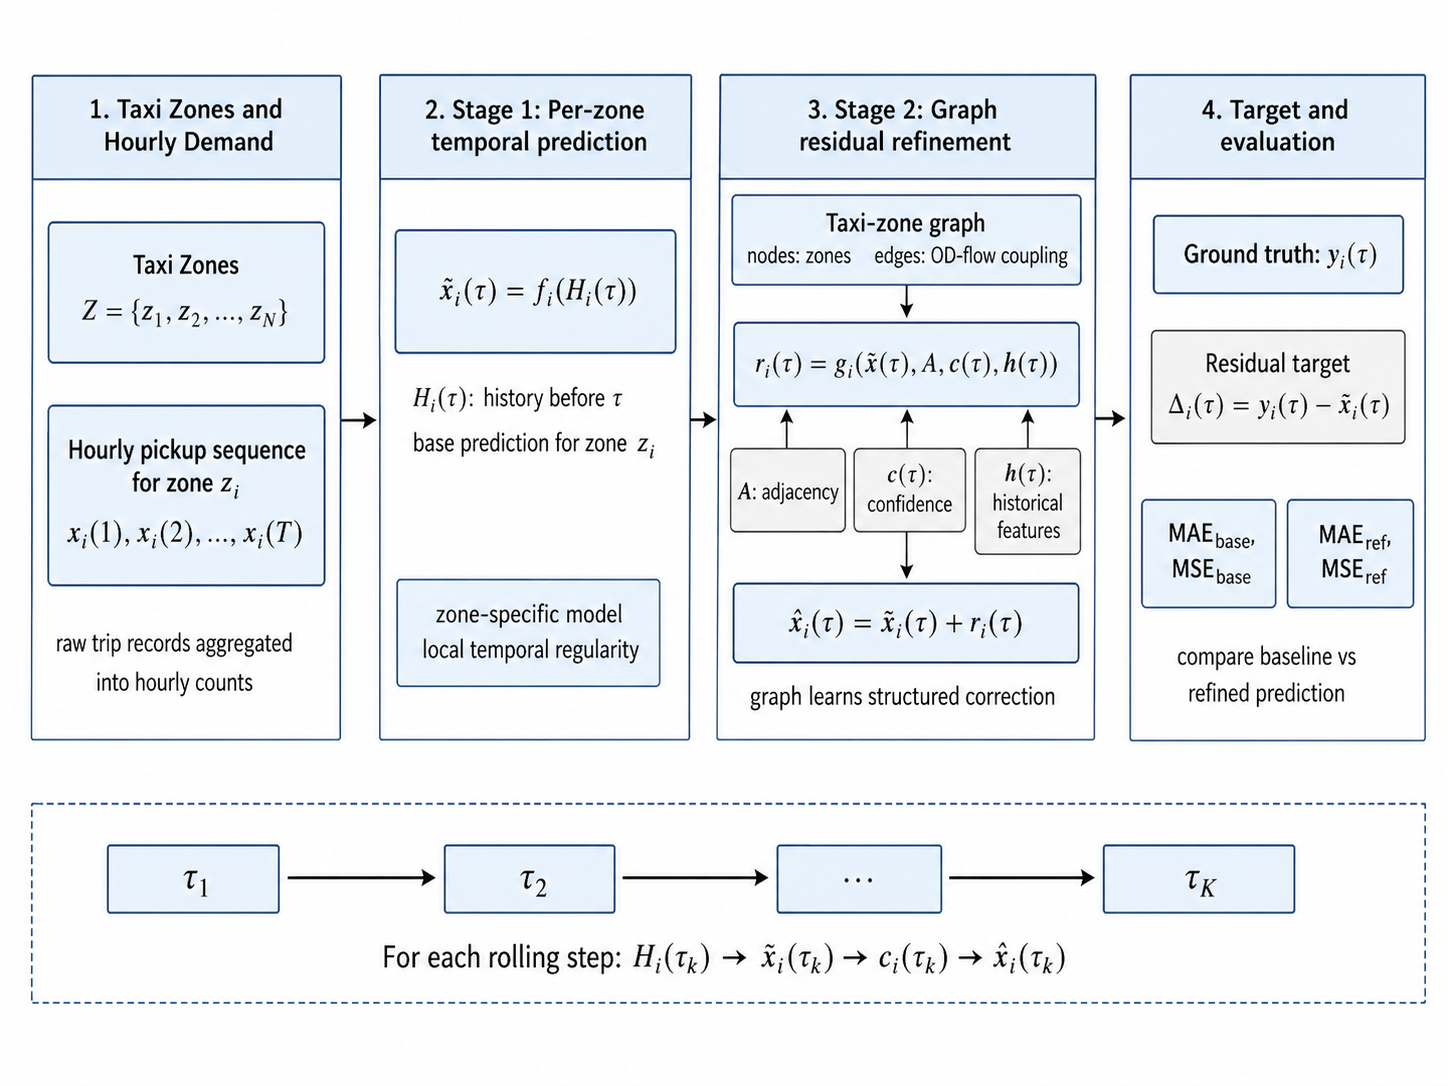
\includegraphics[width=1\textwidth]{img/3.1.png}
	\caption{Illustration of the problem setup used in this thesis. Hourly taxi pickup counts are modelled at the zone level, where a per-zone temporal predictor first generates a base forecast and a graph refinement stage then learns a residual correction on the taxi-zone graph. The framework is evaluated under a rolling forecasting protocol using ground-truth hourly counts and step-wise error metrics.}
	\label{fig:3.1}
\end{figure}

\subsection{Forecasting Objective}

Let the urban system be partitioned into a set of Taxi Zones
\[
\mathcal{Z} = \{z\_1, z\_2, \dots, z\_N\},
\]
where each zone corresponds to a predefined administrative or operational region used in the taxi dataset. For each zone \(z\_i\), the raw data consist of time-stamped trip records with pickup locations. These records are aggregated into hourly counts, producing a univariate temporal sequence
\[
x\_i(1), x\_i(2), \dots, x\_i(T),
\]
where \(x\_i(t)\) denotes the number of taxi pickups observed in zone \(z\_i\) during hour \(t\).

The central forecasting task is next-step prediction at hourly granularity. Given the observed history for zone \(z\_i\) up to time \(t\), the system aims to predict
\[
\hat{x}\_i(t+1),
\]
the demand for the next hour. More generally, for a target timestamp \(\tau\), the prediction problem can be written as
\[
\hat{x}\_i(\tau) = f\_i\big(\mathcal{H}\_i(\tau)\big),
\]
where \(\mathcal{H}\_i(\tau)\) denotes the history available for zone \(z\_i\) strictly before \(\tau\), and \(f\_i(\cdot)\) denotes the temporal predictor associated with that zone.

This thesis does not formulate the temporal stage as a direct multivariate city-wide forecasting model. Instead, the base prediction stage is defined per zone. That is, each zone maintains its own model parameters and its own training history, while spatial interaction is handled later by a separate graph refinement stage. The rationale is that a zone-level forecasting problem has highly local temporal regularities, often shaped by specific functional roles such as residential demand, airport traffic, nightlife, or commuter concentration. Preserving this heterogeneity is methodologically desirable because it reduces the risk that a single monolithic temporal model collapses distinct demand processes into one shared representation.

\subsection{Two-Stage Forecasting Formulation}

The overall method is formulated as a two-stage architecture.

In the first stage, a temporal base predictor produces an initial forecast for each zone:
\[
\tilde{x}\_i(\tau) = f\_i\big(\mathcal{H}\_i(\tau)\big).
\]
This prediction is accompanied by an uncertainty estimate and several auxiliary reliability indicators. The collection of zone-level temporal predictions across all zones forms a vector
\[
\tilde{\mathbf{x}}(\tau) =
[\tilde{x}\_1(\tau), \tilde{x}\_2(\tau), \dots, \tilde{x}\_N(\tau)]^\top.
\]

In the second stage, these temporal predictions are treated as priors on a graph whose nodes correspond to Taxi Zones and whose edges reflect mobility coupling derived from origin-destination flows. The graph model does not predict demand from scratch. Instead, it learns a residual correction:
\[
r\_i(\tau) = g\_i\big(\tilde{\mathbf{x}}(\tau), \mathbf{A}, \mathbf{c}(\tau), \mathbf{h}(\tau)\big),
\]
where \(\mathbf{A}\) denotes the adjacency structure of the graph, \(\mathbf{c}(\tau)\) denotes node-level confidence values, and \(\mathbf{h}(\tau)\) denotes supplementary historical features. The final refined prediction is therefore
\[
\hat{x}\_i(\tau) = \tilde{x}\_i(\tau) + r\_i(\tau).
\]

This residual formulation is important. It assumes that the temporal stage already captures most of the signal that is specific to each zone, while the graph stage contributes structured corrections that account for spatial relationships and cross-zone consistency. The graph model is therefore tasked with learning what the temporal stage missed, rather than rediscovering the entire demand signal from the graph alone. This reduces modelling burden and makes the role of the graph stage more interpretable.

\subsection{Rolling Forecasting Setting}

The forecasting task is evaluated under a rolling protocol rather than a single static train/test split. Let \(\tau\_1, \tau\_2, \dots, \tau\_K\) denote a sequence of target timestamps separated by one hour. At each target hour \(\tau\_k\), the system reconstructs the temporal input windows, generates predictions for all eligible zones, computes confidence scores, applies graph refinement, and stores both zone-level outputs and aggregate error metrics.

Formally, for each rolling step \(k\), the procedure is
\[
\mathcal{H}\_i(\tau\_k) \rightarrow \tilde{x}\_i(\tau\_k)
\rightarrow c\_i(\tau\_k)
\rightarrow \hat{x}\_i(\tau\_k),
\]
for all zones \(z\_i\). This setup is intended to mimic a realistic forecasting workflow, where predictions must be generated repeatedly as time moves forward. It is also methodologically useful because it exposes temporal drift, variation in uncertainty, and the stability of forecasting performance across consecutive operating hours.

\subsection{Target Variables and Evaluation Quantities}

The primary target variable is the observed hourly taxi pickup count in each zone. Let \(y\_i(\tau)\) denote the ground-truth count for zone \(z\_i\) at target hour \(\tau\). The temporal baseline prediction is \(\tilde{x}\_i(\tau)\), and the graph-refined prediction is \(\hat{x}\_i(\tau)\).

At the graph stage, the supervised signal is the residual
\[
\Delta\_i(\tau) = y\_i(\tau) - \tilde{x}\_i(\tau),
\]
rather than the raw target \(y\_i(\tau)\). This is consistent with the residual refinement philosophy described above.

For evaluation, the main scalar error measures are mean absolute error and mean squared error. For a set of valid zones \(\mathcal{V}\_\tau\) at time \(\tau\), the baseline MAE is
\[
\text{MAE}\_{\text{base}}(\tau)
= \frac{1}{|\mathcal{V}\_\tau|}
\sum\_{i \in \mathcal{V}\_\tau}
|\tilde{x}\_i(\tau) - y\_i(\tau)|,
\]
and the refined MAE is
\[
\text{MAE}\_{\text{ref}}(\tau)
= \frac{1}{|\mathcal{V}\_\tau|}
\sum\_{i \in \mathcal{V}\_\tau}
|\hat{x}\_i(\tau) - y\_i(\tau)|.
\]
Similarly, the corresponding mean squared errors are
\[
\text{MSE}\_{\text{base}}(\tau)
= \frac{1}{|\mathcal{V}\_\tau|}
\sum\_{i \in \mathcal{V}\_\tau}
(\tilde{x}\_i(\tau) - y\_i(\tau))^2
\]
and
\[
\text{MSE}\_{\text{ref}}(\tau)
= \frac{1}{|\mathcal{V}\_\tau|}
\sum\_{i \in \mathcal{V}\_\tau}
(\hat{x}\_i(\tau) - y\_i(\tau))^2.
\]

These metrics are stored at each rolling step and can also be aggregated across the full rolling horizon to provide overall performance summaries.

\section{Data Representation and Preprocessing}
\label{sec:data-representation}

\subsection{Raw Data and Hourly Aggregation}

The raw taxi dataset contains individual trip records with at least two essential attributes for this work: pickup timestamp and pickup zone identifier. Since the objective is hourly zone-level demand forecasting, the raw event stream is transformed into a panel of hourly counts. Each trip record contributes one count to the corresponding zone and hour, and all records are aggregated by hour after flooring the timestamps to hourly precision.

For each zone \(z\_i\), this produces a sparse sequence of observed counts over time. However, a forecasting model requires dense temporal input, including explicit zeros for hours in which no pickups were recorded. Therefore, the methodology constructs dense hourly timelines over the relevant historical range. Missing hours are reintroduced with count zero, ensuring that the sequence used by the temporal model preserves both activity and inactivity patterns. This is especially important in sparse zones, where the absence of events is itself informative \cite{zhuang2022sparse,lyu2021bigdata}.

\subsection{Zone Filtering and Data Validity}

Not all Taxi Zones are equally suitable for modelling. In practical taxi datasets, some zones may correspond to special-purpose regions, missing lookup entries, irregular traffic patterns, or insufficient data coverage. The methodology therefore allows the exclusion of selected zones during preprocessing. This prevents invalid or unstable zones from contaminating the temporal model, confidence construction, or graph refinement stage.

The filtering step is intentionally performed early in the pipeline. Once excluded, a zone does not contribute to temporal training, rolling evaluation, or graph refinement. This ensures consistency across all later stages. From a methodological point of view, such filtering reflects a realistic data curation step in applied mobility forecasting, where certain regions may be unusable because of missing metadata, unstable counts, or lack of meaningful demand \cite{lyu2021bigdata}.

\subsection{Temporal Granularity and Historical Windows}

The system operates at hourly granularity throughout. This choice balances temporal detail and computational tractability. Minute-level modelling would be too sparse and noisy for many zones, while daily aggregation would remove the within-day structure that is central to taxi demand \cite{tang2019spatiotemporal,liao2022taxi}. Hourly aggregation preserves immediate fluctuations, daily cycles, and longer periodic patterns in a form that can be handled efficiently by recurrent and attention-based models.

A key methodological decision is to represent the historical sequence at multiple time scales. Instead of feeding one fixed look-back window into a single sequence encoder, the framework constructs four temporal contexts:
\begin{itemize}
	\item a short-term context of the most recent 1 hour,
	\item a daily context of the most recent 24 hours,
	\item a weekly context of the most recent 168 hours,
	\item and a monthly context of the most recent 720 hours.
\end{itemize}

These windows are not arbitrary. The 1-hour view captures immediate local momentum. The 24-hour view reflects intra-day structure and recent daily periodicity. The 168-hour view introduces weekly repetition and the weekday--weekend distinction. The 720-hour view provides roughly one month of context and can represent slower trend evolution. The methodology assumes that these time scales contain complementary information and that explicitly encoding them is preferable to relying on a single model to infer all relevant horizons from one undifferentiated sequence \cite{liao2022taxi,huang2021multiresolution,lim2021survey}.

\subsection{Construction of Dense Zone Series}

For each zone and each forecasting context end time, a dense hourly series is constructed over the relevant history. Let \(\tau\) denote a target hour and let the forecasting horizon be one step. Then the last available hour before prediction is
\[
\tau^- = \tau - 1 \text{ hour}.
\]
The dense zone series is built up to \(\tau^-\). To provide sufficient context for the monthly branch and for sliding-window training, the historical extraction range is extended beyond the basic 720-hour input window. In effect, the method reconstructs a sufficiently long dense hourly sequence ending at \(\tau^-\), allowing both model training windows and the final inference window to be assembled without any future leakage.

For sparse zones, this dense reconstruction is crucial. Without it, the model would see only event times and could not distinguish between a genuinely inactive period and missing data. With explicit zero filling, the temporal encoders can learn the difference between peak hours, moderate demand, and prolonged inactivity \cite{zhuang2022sparse}.

\subsection{Scaling and Temporal Integrity}

Neural sequence models are sensitive to the scale of their inputs. Since demand counts vary considerably across zones, the framework scales each zone independently before building model inputs. A Min--Max scaling transformation is applied:
\[
x\_i^{\text{scaled}}(t)
=
\frac{x\_i(t)-x\_i^{\min}}{x\_i^{\max}-x\_i^{\min}},
\]
with suitable safeguards for degenerate cases such as constant sequences. The use of zone-specific scaling matches the per-zone forecasting design. A high-demand airport zone and a low-demand peripheral zone may have very different count ranges, and scaling them jointly would distort the learning problem.

A methodological requirement here is temporal integrity. The scaler must be fitted only on historical observations available before the target hour. Let \(\tau\) be the prediction time. Then the scaler for forecasting \(\tau\) is fitted on data strictly earlier than \(\tau\). This ensures that neither the scale parameters nor the input windows leak future information. This seemingly technical detail is methodologically important because improper scaling is a common source of hidden leakage in time-series experiments \cite{hewamalage2022pitfalls,cerqueira2020evaluating}.

\subsection{Sliding-Window Sample Generation}

After dense reconstruction and scaling, training samples are produced by sliding windows over the historical series. Let \(L = 720\) denote the total monthly context length and let the prediction horizon be \(H=1\). For each valid starting position \(s\), the full input window is
\[
[x\_i^{\text{scaled}}(s), x\_i^{\text{scaled}}(s+1), \dots, x\_i^{\text{scaled}}(s+L-1)],
\]
and the corresponding target is
\[
y\_i^{\text{scaled}}(s)
=
x\_i^{\text{scaled}}(s+L).
\]

From the full monthly window, the shorter branch windows are extracted from its most recent part:
\begin{align*}
	\mathbf{x}^{1h}\_i(s) &= [x\_i^{\text{scaled}}(s+L-1)],\\
	\mathbf{x}^{1d}\_i(s) &= [x\_i^{\text{scaled}}(s+L-24), \dots, x\_i^{\text{scaled}}(s+L-1)],\\
	\mathbf{x}^{1w}\_i(s) &= [x\_i^{\text{scaled}}(s+L-168), \dots, x\_i^{\text{scaled}}(s+L-1)],\\
	\mathbf{x}^{1m}\_i(s) &= [x\_i^{\text{scaled}}(s), \dots, x\_i^{\text{scaled}}(s+L-1)].
\end{align*}

This construction means that all branches predict the same next-hour target but view the historical sequence at different temporal horizons. The branch inputs are therefore temporally aligned and complementary.

\subsection{Graph Construction from Origin--Destination Flow}

The spatial component of the framework is built from an origin--destination flow matrix rather than a purely geographic adjacency matrix. Each node represents a Taxi Zone, and an edge is created between two zones if the corresponding entry in the OD flow matrix indicates non-zero interaction. Let \(\mathbf{A} \in \mathbb{R}^{N \times N}\) denote the zone-by-zone flow matrix. The graph connectivity used by the graph neural network is derived as
\[
A\_{ij}^{\text{bin}} =
\begin{cases}
	1, & \text{if } A\_{ij} > 0,\\
	0, & \text{otherwise}.
\end{cases}
\]

This binary adjacency is then converted into sparse edge-index form for graph learning. Methodologically, the choice of OD flow over geographic adjacency is important. Geographical closeness does not necessarily correspond to mobility coupling. Two neighbouring zones may have weak travel exchange, while two zones that are geographically farther apart may exhibit strong interaction because of commuting, airport trips, or major transit connections \cite{ke2021od,jiang2022survey}. The OD graph therefore encodes functional linkage rather than mere cartographic proximity.

For the reported causal experiments, non-zero geographic or rolling OD entries define graph connectivity for a mean-aggregation GraphSAGE model. The graph ablation is therefore interpreted as a comparison of alternative graph topologies, with the no-graph temporal prediction as its control.

\subsection{Auxiliary Historical Features for Graph Refinement}

In addition to the base temporal prediction and the confidence score, the graph refinement stage receives auxiliary node-level history summaries. These features are simple averages of the zone demand over selected windows before the target hour:
\begin{align*}
	m\_i^{24h}(\tau) &= \frac{1}{24}\sum\_{h=1}^{24} x\_i(\tau-h),\\
	m\_i^{168h}(\tau) &= \frac{1}{168}\sum\_{h=1}^{168} x\_i(\tau-h),\\
	m\_i^{720h}(\tau) &= \frac{1}{720}\sum\_{h=1}^{720} x\_i(\tau-h).
\end{align*}

These features serve as low-dimensional summaries of recent demand history. Their role is different from that of the multi-scale temporal base model. The temporal model already processes raw sequences to generate the baseline forecast. The graph stage, however, operates on a single graph snapshot at the target hour and therefore benefits from concise contextual descriptors that summarise whether the current zone is typically busy or quiet over short, medium, and long horizons \cite{lyu2021bigdata,lim2021survey}. Before being used by the graph network, these history features are stabilised by replacing missing values and applying a \(\log(1+x)\) transform \cite{akram2023counts}.


\section{Stage One: Temporal Forecasting Candidates}
\label{sec:temporal-stage}

Experiment~1 benchmarks several temporal backbones under the common rolling protocol. TCN is selected as the cached temporal baseline for the causal residual experiments in Chapter~5. The following subsections document the implemented multi-scale candidate, including its inputs and architecture; they should not be read as claiming that multi-scale is the backbone used in Experiments~2--6.

\subsection{Motivation for a Multi-Branch Design}

The multi-scale candidate is trained independently for each zone. Its central design hypothesis is that urban taxi demand cannot be represented adequately by one temporal horizon alone. A purely short-window model may react to recent fluctuations but fail to preserve weekly repetition or slower trends. A purely long-window model may encode broader context but blur immediate local shifts. The candidate therefore uses a multi-branch design in which distinct encoders are assigned to different temporal horizons and their representations are fused before the final prediction step \cite{liao2022taxi,huang2021multiresolution,lim2021survey}.

\begin{figure}[h]
	\centering
	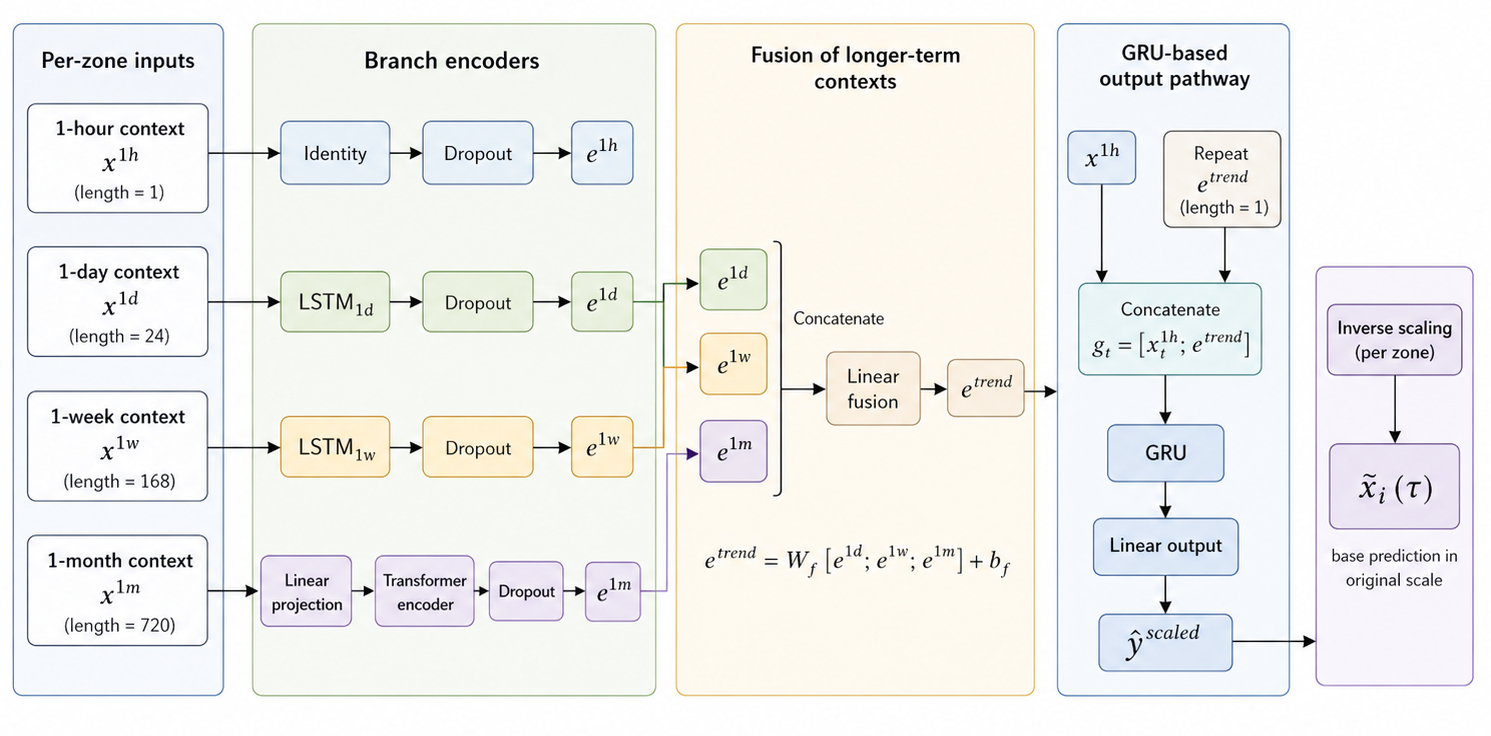
\includegraphics[width=1\textwidth]{img/3.2.png}
\caption{Implemented multi-scale temporal candidate for each taxi zone. Inputs from 1 hour, 1 day, 1 week, and 1 month are encoded by branch-specific modules, fused into a longer-term trend representation, and combined with the short-term signal in a GRU-based output pathway. Chapter~5 compares this candidate with the TCN selected for residual experiments.}
	\label{fig:3.2}
\end{figure}


This architecture is also shaped by the practical nature of the forecasting target. Because the task is one-step-ahead hourly prediction, the system does not need a full sequence-to-sequence decoder. Instead, it needs a compact but expressive representation of recent dynamics that can map directly to the next hour. The branch encoders and fusion module are therefore designed to extract complementary embeddings rather than to reconstruct the whole future trajectory.

\subsection{Per-Zone Temporal Modelling}

Each Taxi Zone is assigned its own temporal forecasting model. The parameter set for each temporal model is zone-specific. The model is trained on the historical sequence of that zone only, and its checkpoint is stored independently from the checkpoints of other zones.

This lets each model specialise to the local temporal signature of its zone, avoids forcing all regions into one shared temporal representation, and supports independent checkpointed incremental updates. The cost is that the system must maintain many separate models rather than one global model, but the framework accepts this trade-off because local specialisation is prioritised at the temporal stage \cite{lim2021survey,zhuang2022sparse}.

\subsection{Branch Inputs}

For each zone, a training or inference example consists of four temporally aligned inputs:
\[
\mathbf{x}^{1h}, \quad
\mathbf{x}^{1d}, \quad
\mathbf{x}^{1w}, \quad
\mathbf{x}^{1m}.
\]
These correspond to the 1-hour, 1-day, 1-week, and 1-month contexts described earlier. Each input is represented as a univariate sequence with one feature channel.

The monthly branch retains the full 720-hour window, the daily and weekly branches use the most recent 24 and 168 elements, and the short branch uses only the most recent hour. Although a length-1 branch is minimal, it serves as the explicit carrier of immediate local momentum when combined with the fused longer-term trend representation inside the GRU pathway.

\subsection{Daily and Weekly Encoders}

The daily and weekly branches are encoded with LSTM networks. For the daily branch, the sequence \(\mathbf{x}^{1d}\) is passed through an LSTM:
\[
\mathbf{h}^{1d} = \text{LSTM}\_{1d}(\mathbf{x}^{1d}),
\]
and the final hidden state is used as the branch embedding:
\[
\mathbf{e}^{1d} = \mathbf{h}^{1d}\_{\text{final}}.
\]
Similarly, the weekly branch is encoded as
\[
\mathbf{e}^{1w} = \text{LSTM}\_{1w}(\mathbf{x}^{1w})\_{\text{final}}.
\]

The use of LSTMs for the 24-hour and 168-hour windows is appropriate because these horizons require ordered-memory modelling but remain short enough for stable recurrent encoding. The daily branch captures within-day structure, while the weekly branch captures weekday--weekend repetition and broader weekly routines \cite{hochreiter1997lstm,jiang2022survey}.

\subsection{Monthly Encoder}

The longest branch, representing roughly one month of hourly history, is encoded differently. Instead of another recurrent network, the methodology uses a Transformer-based encoder after projecting the scalar input into a hidden space. Let the monthly sequence be \(\mathbf{x}^{1m}\). It is first mapped by a linear projection:
\[
\mathbf{u}^{1m}\_t = \mathbf{W}\_p x^{1m}\_t + \mathbf{b}\_p,
\]
producing a hidden representation at each time step. The projected sequence is then processed by a Transformer encoder:
\[
\mathbf{H}^{1m} = \text{Transformer}(\mathbf{U}^{1m}),
\]
and the final time-step output is taken as the monthly branch embedding:
\[
\mathbf{e}^{1m} = \mathbf{H}^{1m}\_{\text{final}}.
\]

The methodological reason for assigning the longest horizon to a Transformer is that self-attention can represent long-range dependencies without forcing information to flow through a fully recurrent chain. Over a 720-hour window, slow drifts and distant periodic cues may be easier to retain in an attention-based representation than in a standard recurrent state alone \cite{vaswani2017attention,zhao2026transformers,kim2025dltimeseries}.

\subsection{Branch-Level Dropout and Representation Stability}

After the branch embeddings are obtained, dropout is applied independently to each branch representation. This serves two purposes. First, it acts as regularisation during training by discouraging over-reliance on any single hidden component. Second, and more importantly for this thesis, it enables Monte Carlo Dropout during inference. Because dropout remains active when stochastic forward passes are required, the variability of the resulting predictions and branch embeddings can be used to estimate uncertainty and branch-level stability \cite{gal2016dropout}.

The methodology therefore treats dropout not only as a standard regularisation device but as an integral component of the confidence estimation strategy. This dual role links the temporal predictor directly to the uncertainty and confidence mechanism described later \cite{gal2016dropout}.

\subsection{Fusion of Longer-Term Temporal Contexts}

The daily, weekly, and monthly embeddings are concatenated and passed through a linear fusion layer:
\[
\mathbf{e}^{\text{trend}}
=
\phi\big(
\mathbf{W}\_f
[
\mathbf{e}^{1d}; \mathbf{e}^{1w}; \mathbf{e}^{1m}
]
+
\mathbf{b}\_f
\big),
\]
where \(\phi(\cdot)\) denotes the hidden nonlinearity implied by subsequent processing and the fusion layer compresses the concatenated multi-scale trend information into a single trend vector.

This fused representation is conceptually important. It is not intended to replace the short-term branch. Instead, it acts as a context vector summarising medium- and long-term behaviour. The design assumes that immediate next-hour prediction should be driven by both local momentum and a broader temporal trend state. The fusion layer therefore converts the three longer-horizon branch embeddings into a unified condition that can support final short-term prediction \cite{huang2021multiresolution,lim2021tft}.

\subsection{GRU-Based Output Pathway}

The final prediction pathway is based on a GRU. The fused trend vector is repeated across the short sequence length and concatenated with the 1-hour branch input:
\[
\mathbf{g}\_t = [x^{1h}\_t ; \mathbf{e}^{\text{trend}}],
\]
which forms the GRU input. Since the short branch length is one in the current implementation, the GRU effectively receives a compact representation that combines the most recent observed demand value with the aggregated trend embedding extracted from the longer branches.

The GRU then produces a hidden representation
\[
\mathbf{h}^{1h}\_{\text{gru}} = \text{GRU}(\mathbf{g}),
\]
and the final prediction is obtained via a linear output layer:
\[
\hat{y}^{\text{scaled}} = \mathbf{W}\_o \mathbf{h}^{1h}\_{\text{final}} + b\_o.
\]

This design is slightly unusual compared with standard recurrent forecasting architectures, because the GRU is not asked to process the entire long history directly. Instead, it acts as the final short-term decision mechanism conditioned on fused longer-term context. Methodologically, this makes the architecture modular: long-term dependencies are handled by branch encoders, while the GRU focuses on converting recent local state and broader trend information into a one-step-ahead prediction \cite{cho2014gru,kim2025dltimeseries}.

\subsection{Prediction in Original Scale}

The model outputs predictions in scaled space, because the training samples are built after Min--Max normalisation. To obtain demand in the original count space, the inverse scaling transform is applied:
\[
\tilde{x}\_i(\tau)
=
\text{Scale}^{-1}(\hat{y}^{\text{scaled}}\_i(\tau)).
\]
Because scaling is fitted separately for each zone and each rolling context using only past observations, the inverse transform remains consistent with the temporally valid training and inference setup.

\subsection{Training Objective for the Temporal Stage}

The temporal stage is trained as a supervised next-step regressor. For a batch of training windows from one zone, let the scaled predictions be \(\hat{y}\_b\) and the scaled targets be \(y\_b\). The main loss is mean squared error:
\[
\mathcal{L}\_{\text{temp}}
=
\frac{1}{B}\sum\_{b=1}^{B}
(\hat{y}\_b - y\_b)^2.
\]

The code structure allows for auxiliary logic related to branch uncertainty, but the dominant supervised objective is still the main one-step regression loss. This choice is reasonable because the ultimate target is a scalar hourly count and the branch encoders are all optimised jointly to minimise next-step prediction error.

\subsection{Optimisation and Early Stopping}

Temporal training uses Adam optimisation with a fixed learning rate and an early-stopping mechanism controlled by patience. Let \(\ell^{(e)}\) denote the training loss at epoch \(e\). The best observed loss is tracked, and training terminates if no improvement is seen over a specified number of epochs. This prevents unnecessary optimisation once the zone-specific model has converged and reduces the chance of overfitting, especially in zones with limited training variation.

Because the temporal stage is performed independently per zone, training efficiency is important. Early stopping reduces wasted optimisation and makes checkpoint generation more practical across many zones. This is one of the reasons a relatively simple next-step objective and moderate hidden dimension are sufficient in the current framework.

\subsection{Checkpointing and Model Persistence}

After training, each zone model is saved together with its scaler and metadata describing the latest context end included in training. This creates a checkpointed forecasting state for that zone. During later rolling steps, the incremental manager loads the checkpoint and updates it when the context advances, rather than retraining from scratch. The methodological benefit is that rolling prediction becomes much closer to a real operational scenario, where models are not typically rebuilt every hour without reason \cite{hewamalage2022pitfalls,cavalcante2024review}.

The incremental design updates a saved checkpoint using new observations when new rolling windows arrive. This keeps the computational benefit of checkpointing while allowing the temporal model to adapt as the rolling context advances. This behaviour is discussed in Section~\ref{sec:rolling-protocol}.

\section{Uncertainty Estimation and Confidence Construction}
\label{sec:uncertainty-confidence}

\subsection{Role of Uncertainty in the Framework}

A key methodological feature of the framework is that predictive uncertainty is not treated merely as an auxiliary diagnostic. Instead, it is actively used to influence downstream graph learning. This is important because the graph stage should not trust every baseline prediction equally. Some zone-level predictions are likely to be stable and informative, while others may be noisy due to sparse history, volatile local demand, or disagreement with neighbouring zones \cite{zhuang2022sparse,wang2024probgnn}. The confidence mechanism is designed to distinguish between these cases.

	The confidence assigned to each zone at each rolling step is built from three sources:
	\begin{enumerate}
		\item a prior score reflecting how much historical data the zone has,
		\item a stability score derived from Monte Carlo Dropout variance,
		\item and a historical consistency score that compares causal 24-hour, 168-hour, and 720-hour demand summaries.
	\end{enumerate}
These components are then fused into a single confidence value that is used as a node-level weight in the graph stage \cite{wang2024gnnuncertaintysurvey,park2022confidenceaware}.


\begin{figure}[h]
	\centering
	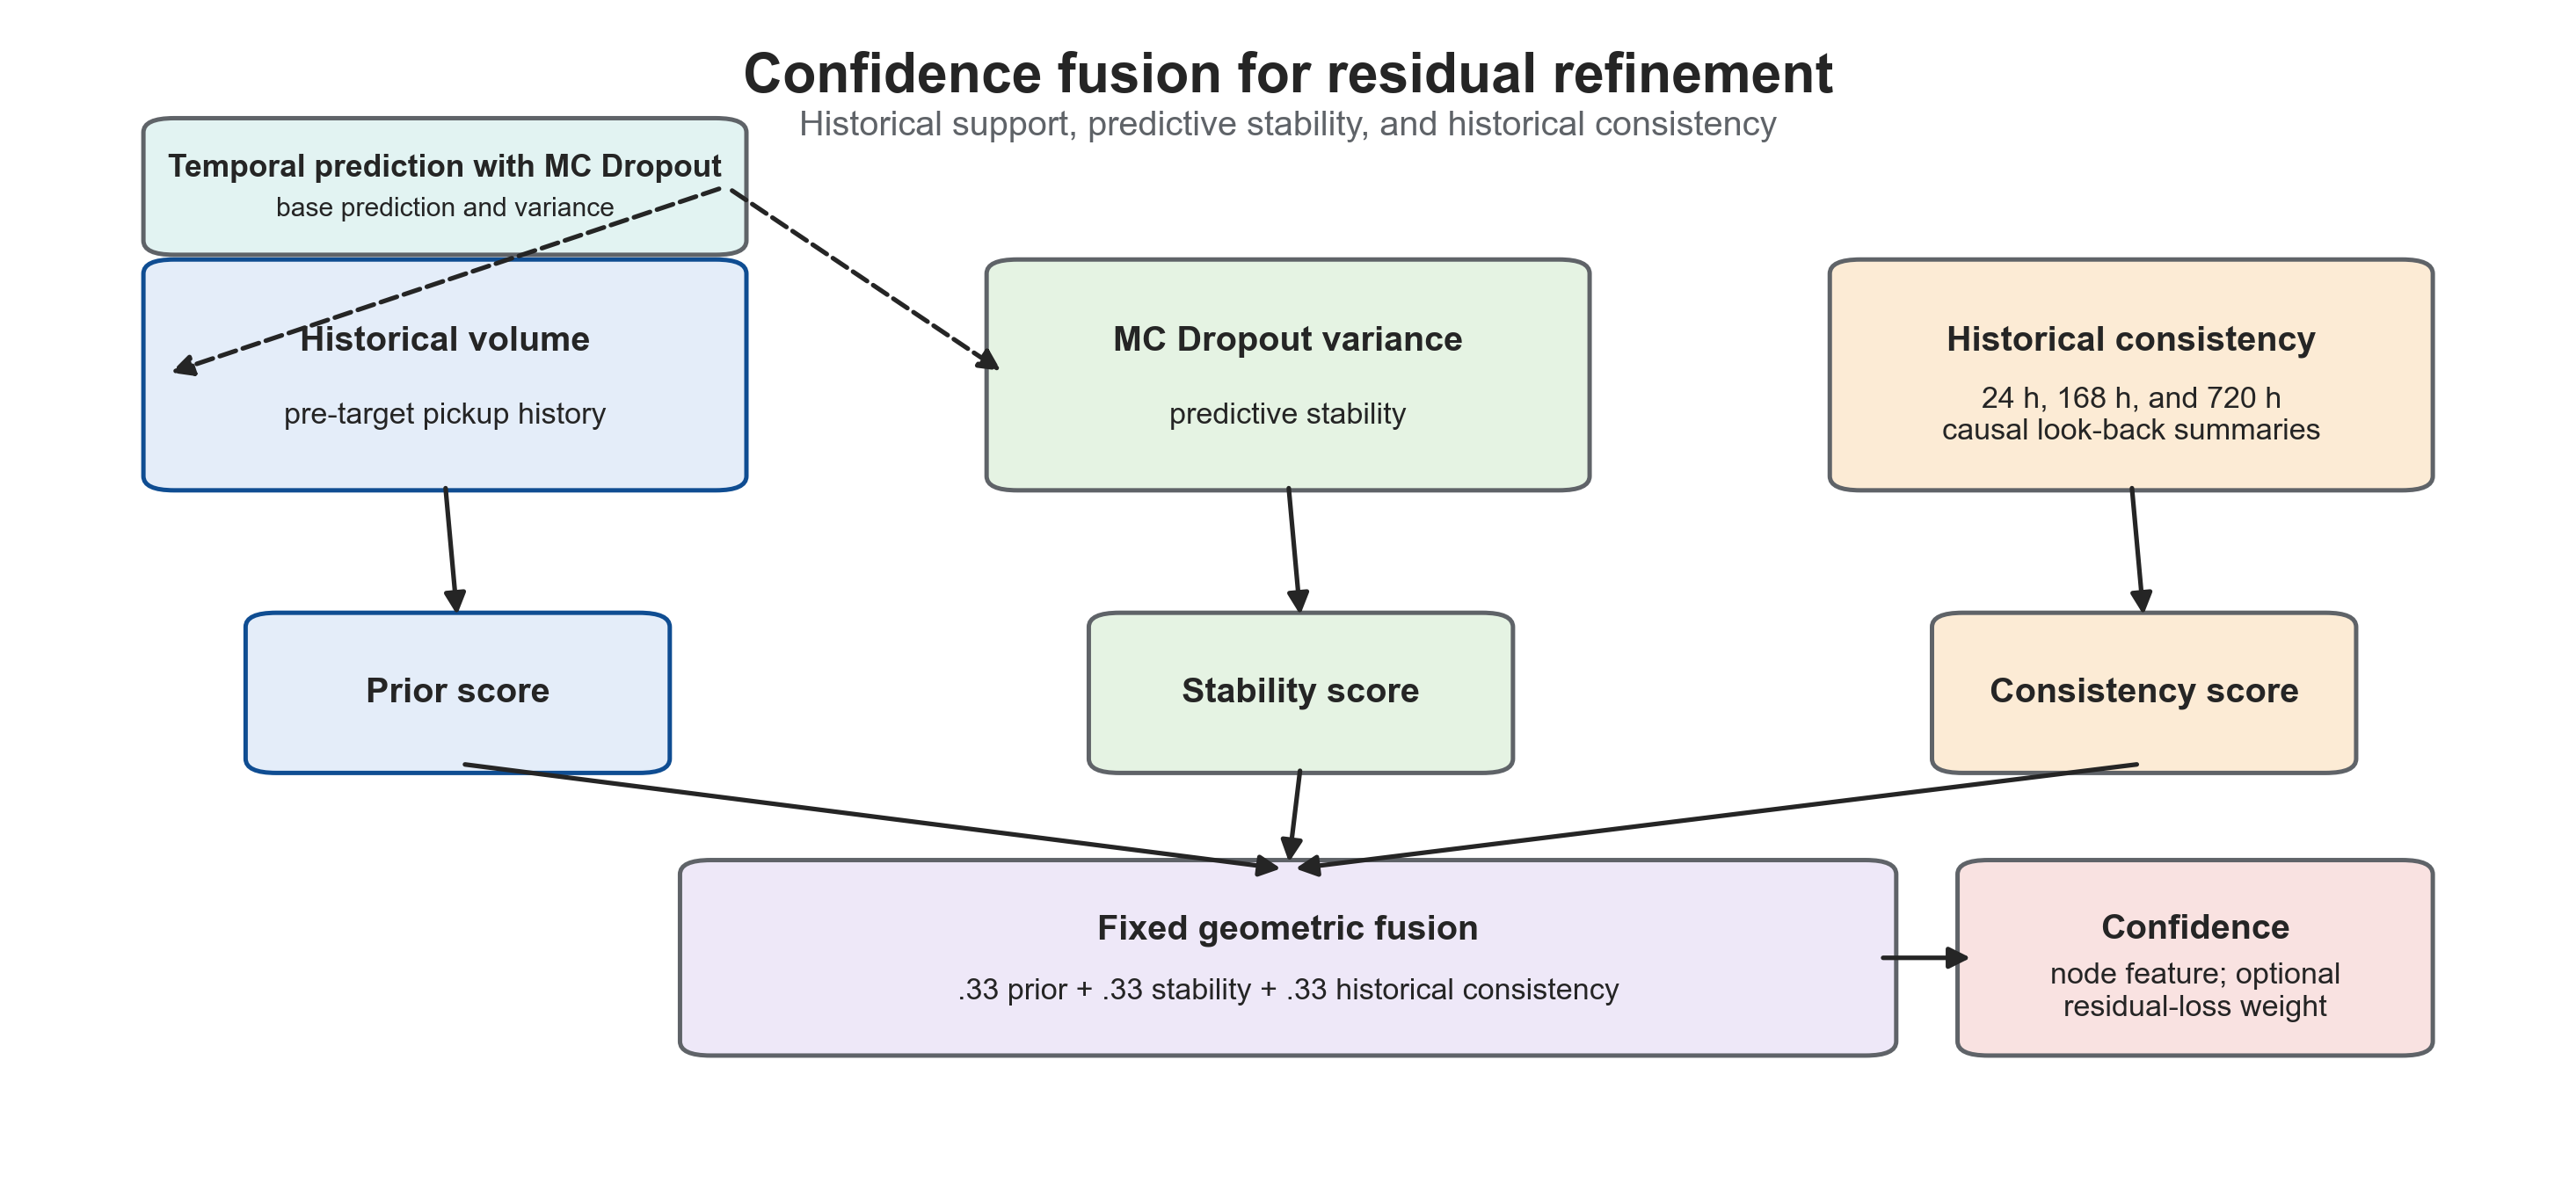
\includegraphics[width=1\textwidth]{img/3.3.png}
	\caption{Confidence construction pipeline. Predictive uncertainty from Monte Carlo Dropout, historical prior information, and historical consistency are fused into a node-level reliability score for graph refinement.}
	\label{fig:3.3}
\end{figure}

\subsection{Monte Carlo Dropout for Predictive Uncertainty}

Monte Carlo Dropout is used to estimate predictive uncertainty in the temporal stage. During inference, dropout remains active, and the same input is passed through the network multiple times. Let
\[
\hat{y}^{(1)}, \hat{y}^{(2)}, \dots, \hat{y}^{(M)}
\]
denote the scaled predictions from \(M\) stochastic forward passes. The predictive mean is
\[
\bar{y}
=
\frac{1}{M}\sum\_{m=1}^{M}\hat{y}^{(m)},
\]
and the predictive standard deviation is
\[
\sigma
=
\sqrt{
	\frac{1}{M}\sum\_{m=1}^{M}
	(\hat{y}^{(m)} - \bar{y})^2
}.
\]

The mean is inverse-transformed to obtain the final point prediction in the original scale. The standard deviation is also mapped back to the original scale using the scaler's data range. This produces a quantity with a direct interpretation in terms of demand-count variability.

Monte Carlo Dropout is attractive here because it does not require a separate probabilistic network or an ensemble of models. It reuses the same architecture and keeps uncertainty estimation computationally feasible even when many zone-specific models must be maintained \cite{gal2016dropout}.

\subsection{Branch-Embedding Variability}

In addition to predictive variance, the framework can inspect the variability of branch embeddings under Monte Carlo sampling. Let
\[
\mathbf{e}^{1h,(m)}, \mathbf{e}^{1d,(m)}, \mathbf{e}^{1w,(m)}, \mathbf{e}^{1m,(m)}
\]
be the branch embeddings from the \(m\)-th stochastic forward pass. Their variance across samples reflects how stable each temporal branch representation is under dropout-induced perturbation.

Although the current downstream confidence mechanism uses overall predictive variance rather than a full branch-specific weighting rule, this embedding variability is still methodologically meaningful. It confirms that the uncertainty process is sensitive not only to the final scalar prediction but also to internal representational instability \cite{gal2016dropout}.

\subsection{Historical Prior Score}

The first component of the confidence mechanism is a prior score that measures how much historical evidence is available for each zone. Zones with richer history are generally easier to model than zones with chronically sparse counts \cite{zhuang2022sparse}. Let \(n\_i\) denote the total number of records or effective count volume associated with zone \(z\_i\) over the available historical data. The prior score is constructed by applying a log transform and min--max normalisation:
\[
p\_i
=
\frac{\log(1+n\_i)-\min\_j \log(1+n\_j)}
{\max\_j \log(1+n\_j)-\min\_j \log(1+n\_j)}.
\]
This score is then rescaled away from exact zero, so that every zone retains at least a minimal confidence level.

The prior score does not depend on the current rolling step. It is a structural quantity reflecting the overall historical sufficiency of a zone. Methodologically, it acts as a regularising anchor: even if a current prediction appears stable under Monte Carlo sampling, a chronically sparse zone should still not be treated with the same confidence as a zone supported by much richer history.

\subsection{Stability Score from Predictive Variance}

The second confidence component is a stability score derived from the predictive variance at the current rolling step. Let \(v\_i(\tau)\) denote the Monte Carlo variance for zone \(z\_i\) at time \(\tau\). Higher variance indicates lower stability. The framework maps this to a score in \((0,1]\) using an exponential decay:
\[
s\_i(\tau)
=
\exp\Big(
-\frac{v\_i(\tau)}{3\lambda\_\tau}
\Big),
\]
where \(\lambda\_\tau\) is a scale factor derived from the median variance across zones at that step. The resulting value is clipped to a small positive lower bound and 1.0 as an upper bound.

This design has two advantages. First, it produces a relative, step-aware notion of stability: what counts as ``high variance'' is interpreted in relation to the current global variance scale. Second, it avoids an overly harsh penalty for moderate uncertainty while still strongly down-weighting extremely unstable predictions. This is appropriate for urban demand forecasting, where some uncertainty is inevitable and should not automatically invalidate a prediction \cite{wang2024probgnn,gal2016dropout}.

\subsection{Historical Consistency Score}

The third component measures agreement among causal historical demand summaries. Let \(m_i^{24h}(\tau)\), \(m_i^{168h}(\tau)\), and \(m_i^{720h}(\tau)\) denote the mean demand over the preceding 24, 168, and 720 hours. Their dispersion is mapped to a bounded score
\[
h_i(\tau)=\exp\left(-\frac{\operatorname{std}\{m_i^{24h}(\tau),m_i^{168h}(\tau),m_i^{720h}(\tau)\}}{d_i(\tau)}\right),
\]
where \(d_i(\tau)\) is a positive scale term. The score is high when short-, medium-, and longer-range history agree and lower when they indicate a changing or unstable demand level. Unlike the earlier neighbourhood-consistency implementation, this component is available without assuming that spatial agreement itself establishes reliability.

\subsection{Confidence Fusion}

The three confidence components are fused multiplicatively in log space:
\[
c\_i(\tau)
=
\exp\Big(
w\_p \log p\_i
+
w\_s \log s\_i(\tau)
+
w\_h \log h\_i(\tau)
\Big),
\]
where \(w\_p\), \(w\_s\), and \(w\_h\) are non-negative weights summing to one. The fixed configuration uses \((0.33,0.33,0.33)\), and Chapter~5 also evaluates searched and learned-softmax variants.

This form of fusion corresponds to a weighted geometric mean rather than an arithmetic mean. Methodologically, that is a sensible choice. If any component is very low, the final confidence should also fall noticeably, because a zone that is historically sparse, highly unstable, or inconsistent across its historical summaries should not remain highly trusted simply because it scores well on one other dimension. The geometric fusion therefore enforces a stricter notion of reliability than a simple additive average.

\subsection{Interpretation of Confidence}

The resulting confidence value
\[
c\_i(\tau) \in (0,1]
\]
has a specific operational interpretation in the methodology. It is not a calibrated probability that the prediction is correct. Rather, it is a relative reliability weight indicating how strongly the graph stage should trust the temporal baseline and the associated residual supervision for that node. A high-confidence node provides a more dependable anchor for graph refinement. A low-confidence node remains in the graph, but its influence on the graph learning objective is reduced \cite{park2022confidenceaware,wang2024gnnuncertaintysurvey}.

The confidence mechanism does not suppress uncertain zones entirely, because uncertain regions may still benefit substantially from spatial correction. Instead, it modulates their influence so that the graph model is shaped more strongly by nodes whose baseline predictions appear trustworthy.

\section{Stage Two: Graph-Based Residual Refinement}
\label{sec:graph-stage}

\subsection{Motivation for Spatial Refinement}

The temporal stage models each zone independently. This is valuable for local specialisation, but it leaves an important weakness unresolved: independent temporal models do not explicitly account for structured interactions between zones. In a mobility system, zones interact through travel flows, commuting patterns, and network effects. If one zone experiences a surge while its strongly connected neighbours do not, the discrepancy may indicate either a true local anomaly or an error in the temporal estimate \cite{jiang2022survey,ke2021od}. The graph stage is introduced precisely to handle this kind of structured interaction.


\begin{figure}[h]
	\centering
	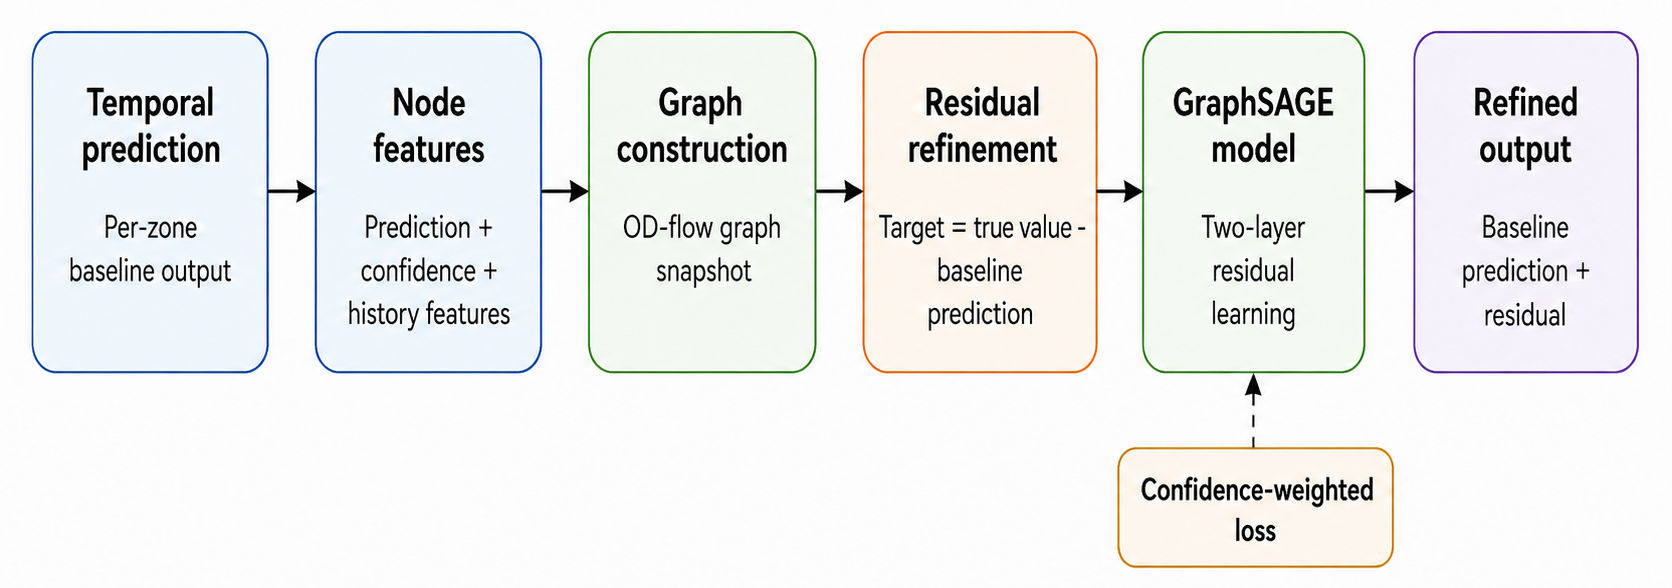
\includegraphics[width=1\textwidth]{img/3.4.png}
\caption{GraphSAGE residual refinement at each rolling step. The taxi-zone graph is built from baseline predictions, confidence scores, historical features, and selected graph connectivity. Confidence is a node feature and an optional residual-loss weight.}
	\label{fig:3.4}
\end{figure}

Rather than building a graph model that predicts demand directly from node features alone, the methodology adopts a residual refinement strategy. The baseline temporal predictions are treated as strong priors, and the graph network learns how much these priors should be adjusted in light of spatial context. This makes the graph stage a corrective mechanism rather than a replacement predictor \cite{shao2022d2stgnn}.


\subsection{Graph Construction from OD Flow Connectivity}

The reported refinement experiments use either geographic adjacency or a rolling OD matrix. For target hour \(\tau\), each rolling OD matrix is constructed from trips strictly before \(\tau\), retaining the top destinations per origin. Its non-zero entries define the available neighbourhood for mean GraphSAGE aggregation. Geographic and OD graph results therefore compare alternative connectivity structures.

\subsection{Node Features}

At each rolling step, the graph is instantiated with one node per valid Taxi Zone. The node feature vector for zone \(z\_i\) at time \(\tau\) is
\[
\mathbf{x}^{\text{graph}}\_i(\tau)
=
[
\tilde{x}\_i(\tau),
c\_i(\tau),
m\_i^{24h}(\tau),
m\_i^{168h}(\tau),
m\_i^{720h}(\tau)
].
\]
If some auxiliary historical features are unavailable, they are replaced safely and transformed using \(\log(1+x)\) before concatenation.

The first element of the node feature vector is the baseline temporal prediction, which also acts as the prior that will later receive residual correction. The second element is the confidence score. The remaining elements summarise historical demand over different temporal ranges. Together, these inputs give the graph network access to the current forecast, the reliability of that forecast, and coarse contextual information about the historical level of the zone \cite{lyu2021bigdata,lim2021survey}.

\subsection{Residual Supervision}

The supervised target for the graph model is not the raw demand count. Instead, it is the residual
\[
r\_i^*(\tau) = y\_i(\tau) - \tilde{x}\_i(\tau).
\]
If the graph model predicts a residual \(\hat{r}\_i(\tau)\), then the final refined prediction is
\[
\hat{x}\_i(\tau) = \tilde{x}\_i(\tau) + \hat{r}\_i(\tau).
\]

The residual strategy stabilises graph learning because the graph model only needs to explain what the temporal stage failed to capture. It also preserves interpretability: a positive residual means underprediction and a negative residual means overprediction \cite{shao2022d2stgnn}.

\subsection{GraphSAGE Architecture}

The graph refinement network is a two-layer GraphSAGE model with mean aggregation. Let \(\mathbf{h}\_i^{(0)} = \mathbf{x}^{\text{graph}}\_i\) be the initial node feature vector.
The aggregation is performed over the selected geographic or rolling OD graph. At each GraphSAGE layer, the node update takes the general form
\[
\mathbf{h}\_i^{(\ell+1)}
=
\sigma\Big(
\mathbf{W}^{(\ell)}
\big[
\mathbf{h}\_i^{(\ell)} \, ; \,
\frac{1}{|\mathcal{N}(i)|}\sum_{j\in\mathcal{N}(i)} \mathbf{h}\_j^{(\ell)}
\big]
\Big),
\]
where \(\text{AGG}\) is mean aggregation, \(\mathbf{W}^{(\ell)}\) is a learnable transformation, and \(\sigma\) is a nonlinear activation. In the implemented design, the activations are followed by dropout and the hidden nonlinearity is GELU.

The first GraphSAGE layer maps the input features into a hidden representation. The second layer further propagates and mixes information across the graph. Finally, a linear output layer projects the hidden state to a scalar residual:
\[
\hat{r}\_i(\tau) = \mathbf{w}\_{\text{out}}^\top \mathbf{h}\_i^{(2)} + b\_{\text{out}}.
\]

The use of mean aggregation is consistent with the overall design goal of smoothing and consistency-aware correction. Because the graph stage is not expected to discover highly complex spatial semantics from scratch, a relatively simple aggregation rule is appropriate and less likely to overfit than more elaborate attention-based alternatives in a limited-data setting \cite{hamilton2017graphsage,jiang2022survey}.

\subsection{Confidence-Aware Loss Weighting}

The graph model is trained using a per-node Smooth \(L\_1\) loss on the residual target:
\[
\ell\_i(\tau)
=
\text{SmoothL1}\big(\hat{r}\_i(\tau), r\_i^*(\tau)\big).
\]
To incorporate reliability information, the loss is weighted by the node confidence:
\[
\mathcal{L}\_{\text{graph}}(\tau)
=
\frac{1}{|\mathcal{V}\_\tau|}
\sum\_{i \in \mathcal{V}\_\tau}
\omega\_i(\tau)\,\ell\_i(\tau),
\]
where the weights \(\omega\_i(\tau)\) are derived from \(c\_i(\tau)\) and normalised so that the mean weight remains close to one.

This weighting strategy is a central methodological innovation of the framework. It allows the graph stage to learn more strongly from nodes whose baseline predictions appear reliable and to down-weight the contribution of unstable or poorly supported nodes. Importantly, this does not mean that low-confidence nodes are ignored. They still receive refined predictions through message passing, but their residual targets influence optimisation less strongly \cite{park2022confidenceaware,wang2024gnnuncertaintysurvey}.

\subsection{Confidence Weighting}

Confidence is available as a node feature and is optionally used to reweight the residual loss. It is not converted into a pairwise edge weight in the reported runs. This allows the experiments to distinguish graph-topology choices from node-level reliability weighting \cite{west2025weighted,hu2025uncertaintygnn}.

\subsection{Graph Training per Rolling Step}

At target hour \(\tau\), the graph stage is trained on residual snapshots with labels strictly earlier than \(\tau\). The current graph contains causal node features and is used only for residual inference and evaluation. If no earlier residual snapshot is available, the system falls back to the temporal prediction and the observation is reported separately from active-refinement summaries. The graph model is optimised with Adam and a cosine annealing learning-rate schedule.

This protocol prevents target-hour demand labels from entering graph supervision. It makes the graph correction task harder than within-hour node interpolation, but it provides evidence that is appropriate for rolling one-hour-ahead forecasting \cite{hewamalage2022pitfalls,cerqueira2020evaluating}.

\subsection{Handling Missing and Invalid Nodes}

Only nodes with valid baseline predictions and valid labels are used in graph training. If a zone is missing a temporal prediction or lacks a valid target value, it is excluded from the graph snapshot for that step. The adjacency structure is then reindexed to match the filtered node set. This avoids contaminating the graph stage with invalid entries and prevents propagation of undefined values.

Such filtering is methodologically justified because the graph stage is a refinement model, not a data imputation mechanism. Its purpose is to improve valid baseline predictions through spatial consistency, not to invent supervision where none exists. Restricting the graph to valid nodes therefore keeps the learning problem well-posed.

\section{Rolling Forecasting Protocol and Model Management}
\label{sec:rolling-protocol}

\subsection{Rolling Workflow}

The entire framework is executed under a rolling protocol. Let the first target time be \(\tau\_1\). For each rolling step \(k = 1, 2, \dots, K\), the target hour is
\[
\tau\_k = \tau\_1 + (k-1)\Delta,
\]
where \(\Delta = 1\) hour. At each step, the system performs the following operations:
\begin{enumerate}
	\item determine the valid historical context for each zone,
	\item train or load the temporal model as required,
	\item generate Monte Carlo baseline predictions and uncertainty estimates,
\item compute prior, stability, and historical-consistency confidence components,
	\item assemble the graph snapshot with node features and residual targets,
	\item train the graph refinement model and produce refined predictions,
	\item compute and save per-hour and cumulative metrics.
\end{enumerate}

This repeated procedure is intended to approximate operational forecasting, in which predictions are updated continuously as time progresses. It also reveals whether the forecasting quality is stable, improving, or deteriorating over the rolling horizon \cite{hewamalage2022pitfalls,cerqueira2020evaluating}.

\subsection{Incremental Update Mechanism}

The framework uses an incremental training manager. When new rolling windows become available, the previously trained zone model is updated through lightweight additional optimisation rather than being retrained from scratch. The aim is to preserve most of the learned structure while allowing the model to absorb newly observed data.

Methodologically, this incremental mode occupies an intermediate position between full retraining and static checkpoint reuse. Full retraining is the most adaptive but computationally costly. Pure persistence is computationally cheap but may become stale. Incremental updating attempts to combine the strengths of both: the model retains past knowledge but can respond to drift through targeted adaptation \cite{cavalcante2024review}.

It is important to state the scope of this feature accurately. The incremental mechanism is the sole multi-scale backend and is used by the multi-scale configuration in Experiment~1. Experiments~2--6 reuse cached TCN forecasts and therefore do not execute a multi-scale manager.

\subsection{Why Rolling Evaluation Matters}

Rolling evaluation is not merely an implementation preference. It is a methodological stance about how forecasting systems should be assessed. In static train/test settings, the system is typically trained once and evaluated on a fixed hold-out set. That can be useful for benchmarking, but it suppresses several issues that matter in practice: how performance changes over time, whether uncertainty grows under drift, whether one-step models remain stable across many consecutive operating hours, and what the repeated computational burden of forecasting looks like \cite{hewamalage2022pitfalls,cerqueira2020evaluating}.

By contrast, the rolling protocol used here repeatedly reconstructs the forecasting state as the target time moves forward. This makes the evaluation more realistic and reveals whether graph refinement, uncertainty, and confidence weighting remain useful under changing conditions \cite{hewamalage2022pitfalls}.

\subsection{Temporal Integrity Under Rolling Forecasting}

A forecasting methodology must ensure that only historically available information is used at each step. The current design enforces this in several ways. The temporal input windows end at the hour immediately before the target. The scaler is fitted using observations strictly earlier than the target hour. Historical summary features for graph refinement are computed from windows preceding the target. As a result, the temporal baseline stage is close to a valid leakage-free rolling forecasting procedure \cite{hewamalage2022pitfalls,cerqueira2020evaluating}.

The causal experimental configuration applies the same temporal-integrity principle to graph refinement: graph residual supervision is drawn only from earlier labelled snapshots. The first target step of each rolling window consequently has no residual correction and is treated separately in the reported summaries.

\section{Methodological Discussion}
\label{sec:methodological-discussion}

\subsection{Why the Method Uses a Two-Stage Rather Than End-to-End Design}

A natural question is why the framework is split into a temporal predictor and a graph refiner instead of using a fully end-to-end spatiotemporal graph neural network from the start. There are several methodological reasons. First, a two-stage design makes the role of each component clearer. The temporal stage is responsible for local next-hour forecasting based on historical demand, while the graph stage is responsible for spatial correction. Second, this separation allows the temporal and graph models to be analysed independently. For example, one can compare the temporal baseline to the graph-refined output directly. Third, the two-stage design simplifies engineering and checkpoint management, especially when the temporal stage is maintained per zone.

There is also a conceptual advantage. Many urban forecasting problems contain both strong local regularity and strong spatial coupling, but not always in equal measure. A unified end-to-end model may entangle these two sources of information in ways that are difficult to interpret. The present method deliberately assigns local regularity to the temporal model and structured cross-zone adjustment to the graph model. This division is simple, interpretable, and consistent with the deployment setting \cite{garcia2023explainability,shao2022d2stgnn}.

\subsection{Current Limitations}

The present methodology is strong in several respects, but it also contains deliberate limitations that should be acknowledged clearly.

First, the causal graph protocol depends on a finite history of labelled residual snapshots. It does not establish cross-city or long-horizon generalisation, and its first prediction step cannot receive a residual correction. These constraints are made explicit in Chapter~5 \cite{hewamalage2022pitfalls,cerqueira2020evaluating}.

Second, the reported graph comparison uses hand-specified geographic and OD topologies, including a look-back window, minimum-flow filter, and top-\(k\) retention rule for OD connectivity. Learned or explicitly time-conditioned edge weights remain open extensions \cite{west2025weighted,jiang2022survey}.

Third, the temporal stage is per zone, which improves local specialisation but sacrifices direct parameter sharing across zones. In data-poor zones, a shared or hybrid temporal representation may eventually prove beneficial \cite{lim2021survey,zhuang2022sparse}.

Fourth, the incremental manager is the only multi-scale configuration used in this thesis. Experiments~2--6 use cached TCN forecasts. These modes should be reported separately rather than described as one common temporal configuration.

Fifth, the historical summary features used in the graph stage are deliberately simple. More expressive exogenous variables such as weather, holidays, events, road disruptions, or land-use descriptors are not yet included. Their absence makes the current method cleaner and easier to interpret, but also leaves performance on the table \cite{lyu2021bigdata,demandfeatures2023}.

\subsection{Summary}

In summary, the methodology constructs a rolling two-stage forecasting system for hourly Taxi Zone demand prediction. Experiment~1 benchmarks the implemented multi-scale candidate alongside other temporal backbones and selects TCN for causal residual experiments. The second stage is a GraphSAGE residual refiner evaluated on geographic and rolling OD graph topologies. Between them lies a confidence mechanism that fuses historical sufficiency, predictive stability, and historical consistency into a node-level reliability signal. The rolling protocol provides deployment-oriented evaluation.

The resulting framework is methodologically coherent because each component serves a distinct purpose and because the information flow between components is explicit. Multi-scale modelling addresses temporal heterogeneity. Monte Carlo Dropout quantifies uncertainty. Confidence weighting links uncertainty to downstream optimisation. Graph refinement corrects independent zone-level forecasts using relational structure. Rolling execution tests whether all of these choices remain useful as time advances.

Although the current design still leaves room for repeated graph trials, alternative edge-weight definitions, and more systematic online adaptation, it provides a structured response to temporal complexity, spatial dependence, uncertainty, and operational realism in urban taxi demand forecasting.

	\chapter{Implementation}
	
\section{Overview}

This chapter distinguishes the prototype rolling pipeline from the causal experiment runners that produce the results in Chapter~5. The prototype driver \path{demo_rolling_GNN.py} and Experiment~1 both use \texttt{persistent\_multiscale\_incre\_confi.py} when the multi-scale backend is selected. The prototype is not the source of the reported causal graph results because it can construct and fit a graph on the current labelled snapshot. Experiments~2--6 are generated by \texttt{experiment\_2\_from\_tcn.py} through \texttt{experiment\_6\_from\_tcn.py}; these runners reuse cached no-graph TCN forecasts, form graph-training data from earlier residual snapshots only, and evaluate the current target hour separately.
	
	\begin{figure}[h]
		\centering
		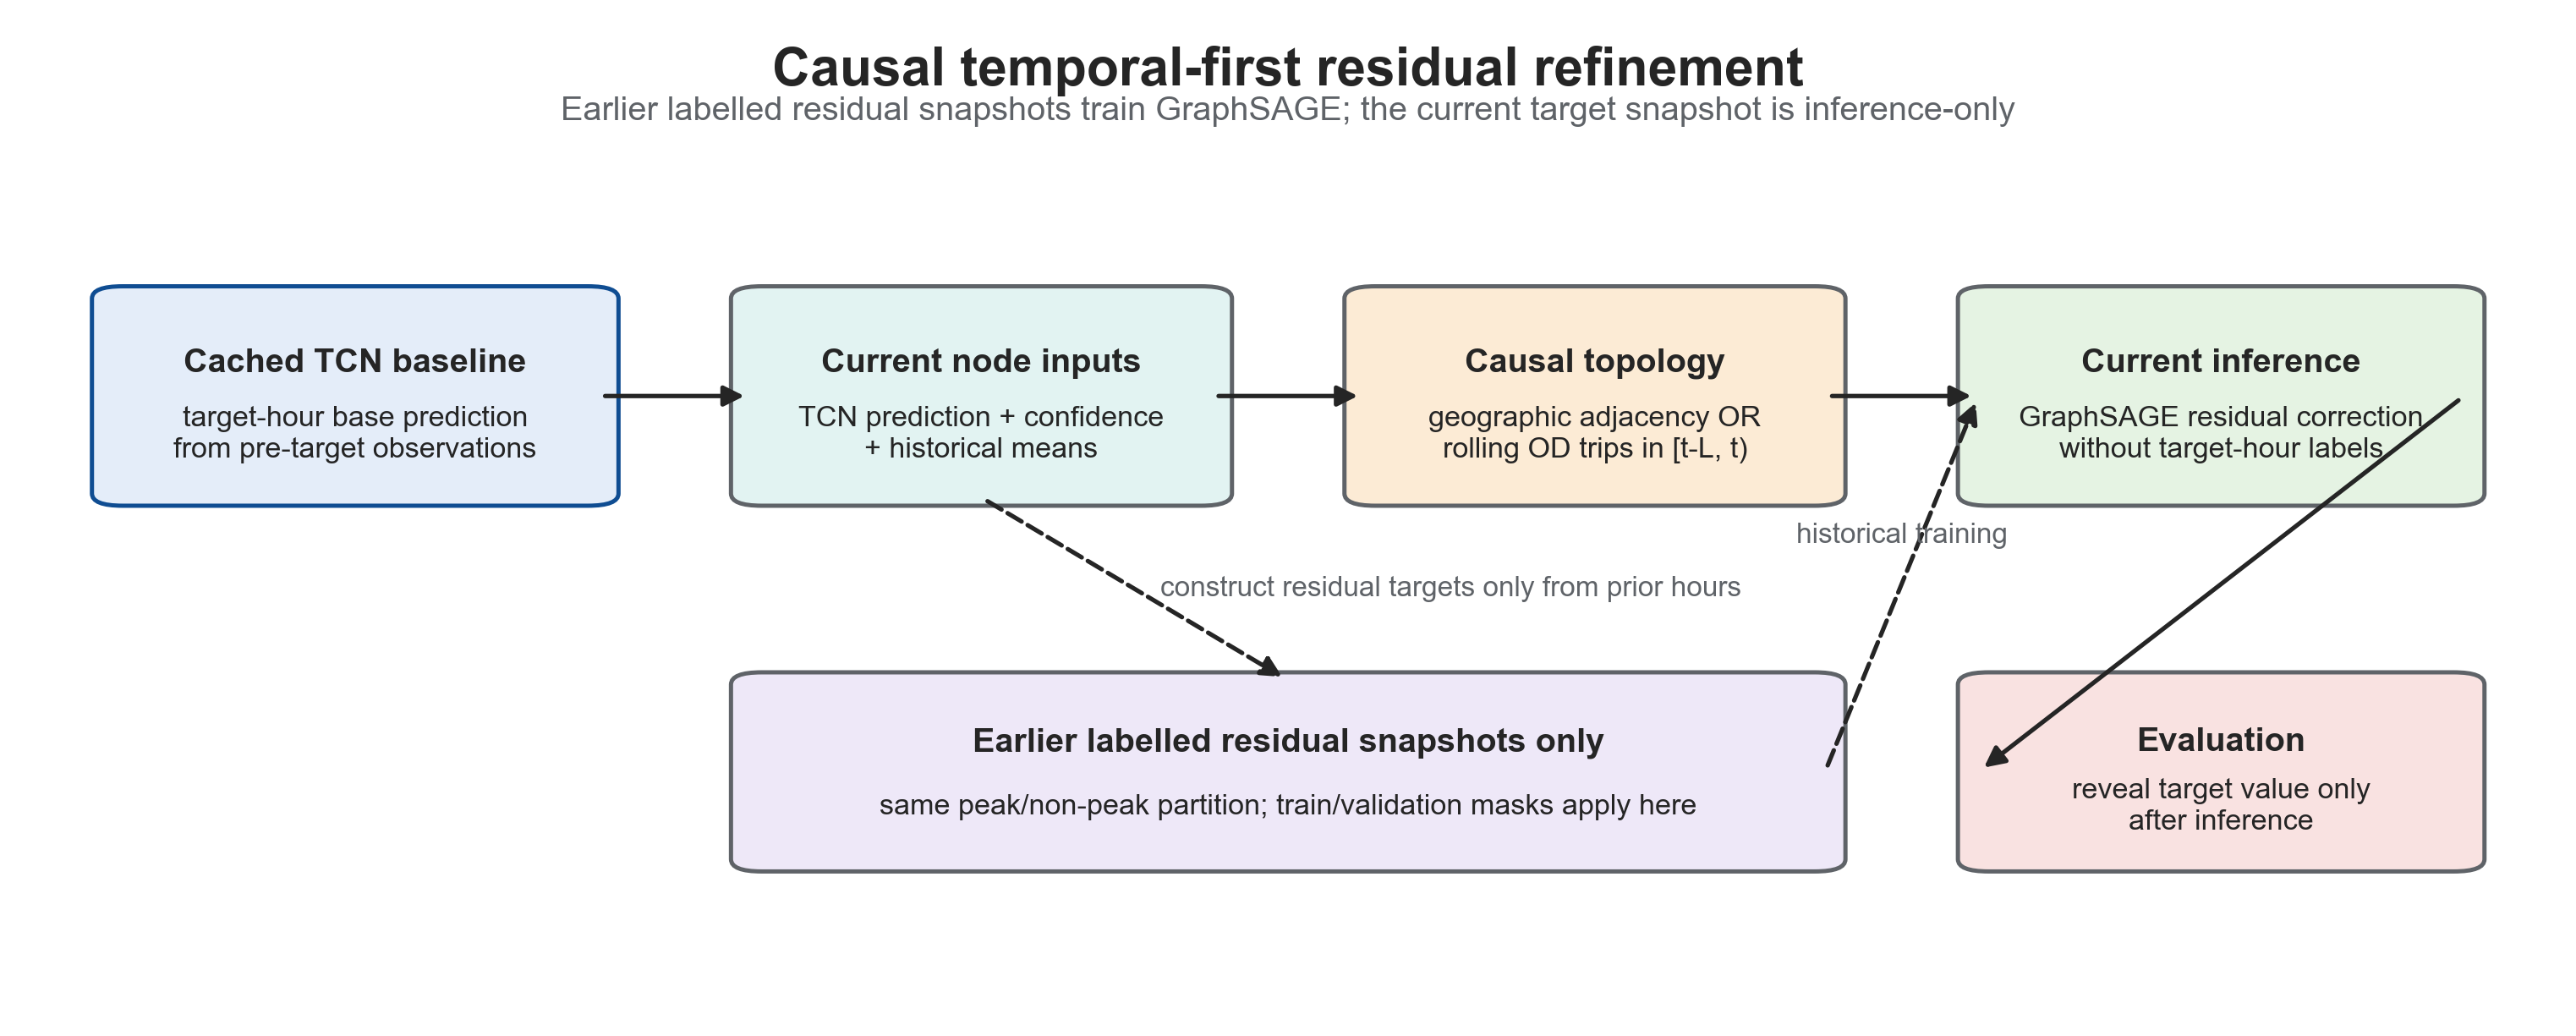
\includegraphics[width=1\textwidth]{img/4.1.png}
		\caption{Causal graph-based residual refinement at each rolling step. The hourly taxi-zone graph is built from valid nodes, baseline predictions, confidence scores, historical features, and selected graph connectivity. A two-layer GraphSAGE model learns residual corrections that are added to the temporal baseline; confidence is a node feature and optional residual-loss weight.}
		\label{fig:4.1}
	\end{figure}
	
	The implementation follows a deliberately modular structure. The temporal stage is isolated inside a model-manager class so that training, checkpoint storage, loading, scaling, inference, and uncertainty estimation are all handled through a consistent interface. The graph stage is separated into its own pipeline so that it receives a clean table of predictions, labels, historical features, and confidence values from the rolling driver. The driver script then coordinates the two stages at each target hour. This design makes the system easier to debug and to extend: the temporal model can be modified without rewriting the graph refinement function, and the graph refinement logic can be changed without altering the data loading and rolling orchestration code.
	
	A central implementation decision is that the rolling pipeline is treated as the main execution unit. The system is not written as a single train-then-test script. Instead, the driver iterates over target timestamps, generates per-zone predictions, evaluates the temporal baseline, constructs the graph input for that hour, performs graph refinement, and stores both detailed and aggregated metrics. The rolling configuration is controlled by explicit constants in the driver script, including paths for the data, lookup table, edge-weight matrix, checkpoint directory, starting target time, number of rolling steps, excluded zones, whether to retrain each hour, and the number of Monte Carlo Dropout samples.
	
\section{Software Structure and Module Responsibilities}
	
		\begin{figure}[h]
		\centering
		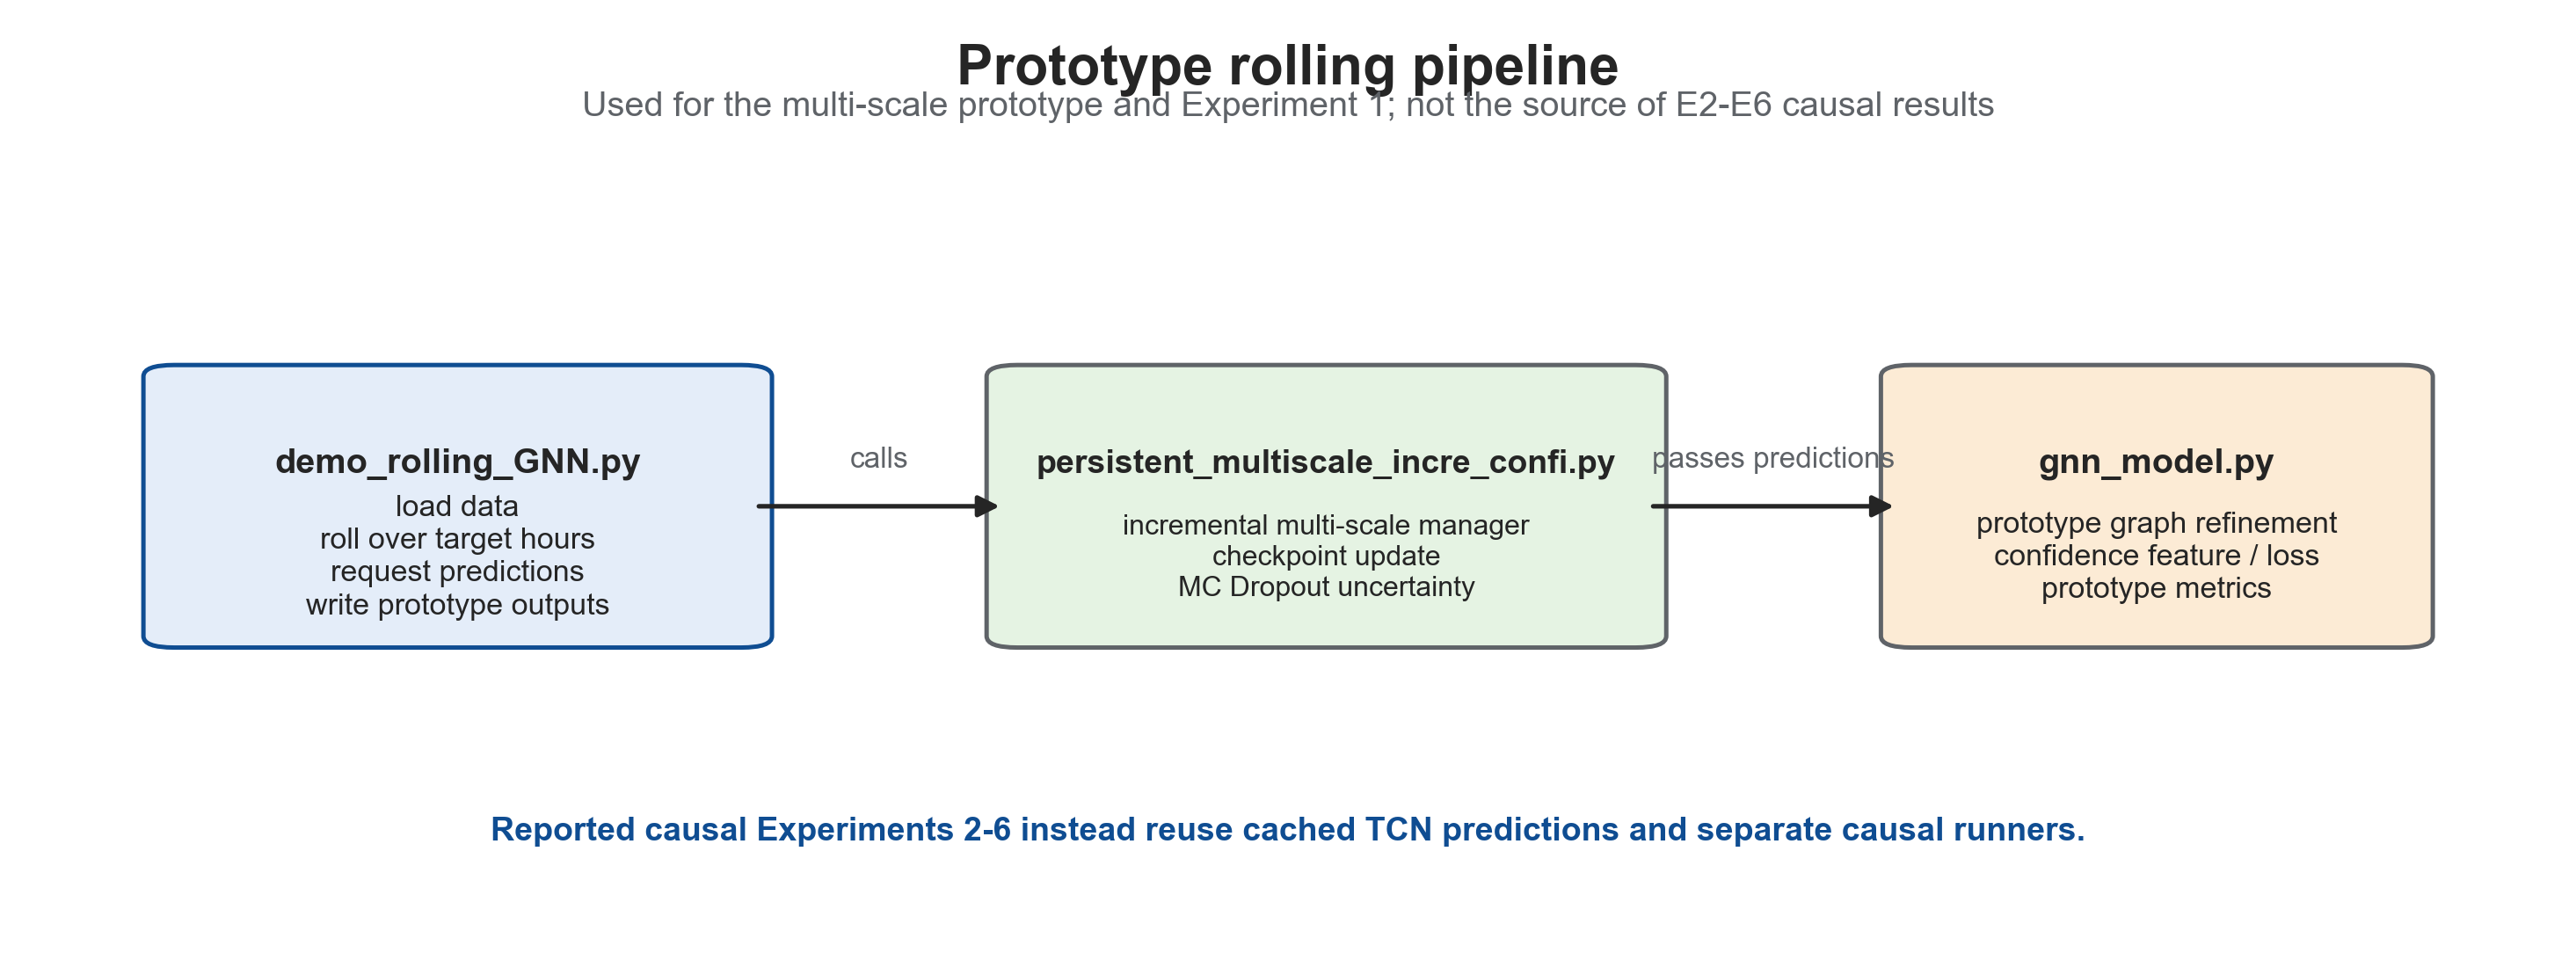
\includegraphics[width=1\textwidth]{img/4.2.png}
		\caption{Overall workflow of the rolling GNN prediction pipeline, showing data preparation, multiscale temporal prediction, and GraphSAGE-based refinement with confidence weighting.}
		\label{fig:4.2}
	\end{figure}
	
\subsection{Prototype Top-Level Rolling Driver}
	
	The main entry point of the implementation is \texttt{demo\_rolling\_GNN.py}. This file is responsible for system-level orchestration rather than model definition. Its responsibilities can be divided into five groups: data preparation, graph support construction, confidence computation, rolling prediction, and output generation.
	
	The first group concerns data preparation. The function \texttt{prepare\_df()} loads \texttt{data.parquet}, keeps the \texttt{pickup\_datetime} and \texttt{PULocationID} columns, converts timestamps into pandas datetime format, floors them to hourly resolution, filters out excluded zones, and prints basic timestamp diagnostics. In addition, \texttt{\_build\_zone\_hourly\_counts()} constructs a grouped count series indexed by \texttt{PULocationID} and hour, which is later used for historical mean features. This implementation choice ensures that the downstream pipeline receives a consistent hourly representation of the raw trip data.
	
	The second group concerns lookup and adjacency construction. The function \texttt{\_load\_zone\_lookup()} reads the taxi-zone lookup table and removes duplicate \texttt{LocationID} entries. The function \texttt{\_build\_zone\_adjacency()} reads the OD flow matrix, normalises possible byte-order marks in row and column labels, maps zone names to \texttt{LocationID} values, and creates an adjacency list by retaining neighbours whose flow weight is greater than zero. This adjacency list is used mainly for the neighbourhood consistency component of the confidence score.
	
	The third group concerns confidence computation. The rolling driver computes three reliability components: a prior score based on historical sample richness, a stability score based on Monte Carlo predictive variance, and a neighbourhood consistency score based on agreement with adjacent zones. The prior score is computed from log-transformed zone counts and then rescaled to avoid exact zero confidence. The stability score is computed from variance values in the current rolling step using an exponential decay controlled by the median variance scale. The neighbourhood score compares each prediction with available predictions from graph neighbours and maps the difference into a clipped confidence interval. These components are combined in log space with weights for prior, stability, and neighbourhood terms, and the resulting score is assigned back to the per-hour prediction dataframe.
	
	The fourth group concerns rolling execution. The function \texttt{run\_rolling\_with\_gnn()} is the central loop. It iterates over \texttt{ROLLING\_STEPS}, constructs the target timestamp for each step, optionally creates a separate checkpoint directory if hourly retraining is enabled, and otherwise reuses the shared temporal manager. For every zone, it calls the temporal manager to train or load the model if needed, obtains the point prediction and uncertainty estimate, records the true value for the current target hour, and computes historical mean features. After the zone loop finishes, it evaluates the baseline temporal predictions, prepares the GNN input table by renaming \texttt{y\_pred} to \texttt{Prediction} and \texttt{y\_true} to \texttt{True Value}, and calls \texttt{run\_gnn\_pipeline()} with the confidence dictionary and historical feature columns.
	
	The fifth group concerns output generation. The rolling driver stores the per-zone temporal predictions in \texttt{predictions\_rolling\_mc.csv}, the temporal baseline hourly metrics in \texttt{hourly\_metrics\_gru.csv}, the graph-refined predictions in \texttt{gnn\_refined\_predictions.csv}, and the graph-stage hourly metrics in \texttt{hourly\_metrics\_gnn.csv}. It also computes overall MAE and RMSE for the temporal baseline and graph-refined outputs and writes them into \texttt{overall\_metrics\_gnn.txt}. The \texttt{main()} function ties these components together by cleaning old checkpoint directories, selecting CUDA or CPU, preparing the dataframe, computing prior scores, loading the lookup table, building adjacency, constructing hourly count series, creating the temporal manager, and launching the rolling loop.
	
\subsection{Incremental Multi-Scale Temporal Manager}
	
	The temporal modelling code used in this thesis is implemented in \texttt{persistent\_multiscale\_incre\_confi.py}. It is a confidence-weighted multi-scale trainer with MC Dropout confidence logic and incremental fine-tuning as the rolling context advances.
	
	The main model class is \texttt{MultiScaleModel}. It is a four-branch temporal architecture with LSTM encoders for daily and weekly contexts, a Transformer encoder for the monthly context, dropout layers for Monte Carlo sampling, a fusion layer, a GRU backbone, and a final linear output layer. The branch-level components are initialised directly inside the constructor. The model encodes the daily, weekly, and monthly branches through \texttt{\_encode\_temporal\_branches()}, where the daily and weekly sequences are passed through LSTM layers, while the monthly sequence is projected and processed through a Transformer. The fused trend representation is concatenated with the short-term one-hour input to build the GRU input, and the final forward pass returns both the scalar prediction and the internal branch embeddings.
	
	The same class also provides two MC Dropout-related interfaces. The function \texttt{mc\_branch\_embeddings()} runs repeated stochastic forward passes and collects branch embeddings under active dropout. The function \texttt{mc\_predict()} returns the mean and standard deviation of repeated stochastic predictions in scaled space. These methods allow the implementation to use the same model both as a point predictor and as an uncertainty estimator.
	
	The manager class, \texttt{MultiScaleModelManager}, wraps the model architecture with persistence, data preparation, scaling, training, inference, and orchestration logic. Its configuration is represented by the \texttt{ManagerConfig} dataclass, which specifies the hidden size, full-training epochs, patience, learning rate, sequence length, forecast length, dropout probability, auxiliary coefficient, and Monte Carlo sample counts. The manager constructor creates the checkpoint directory and stores the duration mapping for the four input branches: 1 hour, 24 hours, 168 hours, and 720 hours.
	
	Persistence is implemented through separate paths for the model weights, scaler, and metadata. The manager checks whether both model and scaler files exist before deciding whether a checkpoint is available. It saves model parameters with \texttt{torch.save}, serialises the scaler with pickle, and stores the latest training context end in a JSON metadata file. This separation makes the checkpoint explicit and recoverable: the learned network state, scaling transformation, and training horizon are all stored independently.
	
\subsection{Causal Graph Refinement Module}
	
	The graph refinement stage is implemented in \texttt{gnn\_model.py}. The file imports \texttt{Data}, \texttt{SAGEConv}, and \texttt{dense\_to\_sparse} from PyTorch Geometric, indicating that the graph stage is built on sparse graph data structures rather than dense matrix operations. The core graph model is \texttt{MultiScaleGraphSAGE}, a two-layer mean-aggregation GraphSAGE network with GELU activations, dropout, and a final linear layer. Its forward pass reads node features and edge indices, retrieves \texttt{base\_pred}, applies two GraphSAGE layers, predicts a residual, and returns both the residual and the refined prediction obtained by adding the residual to the base prediction.
	
The reported causal configuration uses a two-layer mean-aggregation GraphSAGE model. The causal runners construct separate historical training data and current inference data, apply train/validation masks only to the historical snapshots, and use current target labels only after inference to compute metrics. Geographic and OD matrices define the graph topology used for message passing in the reported runs.
	
	\section{Data Loading and Preprocessing Implementation}
	
	The implementation begins with a compact but important preprocessing step. The raw taxi data are loaded from \texttt{data.parquet}. Only the pickup timestamp and pickup zone identifier are required at this stage. The timestamp is converted to pandas datetime format and then floored to the nearest hour, creating the \texttt{datetime} column used throughout the rest of the system. Excluded zones are filtered immediately so that invalid or unwanted regions do not appear in any later computation. This early filtering is important because the same zone set is used for temporal prediction, confidence scoring, graph refinement, and metric aggregation.
	
	
	\begin{figure}[h]
		\centering
		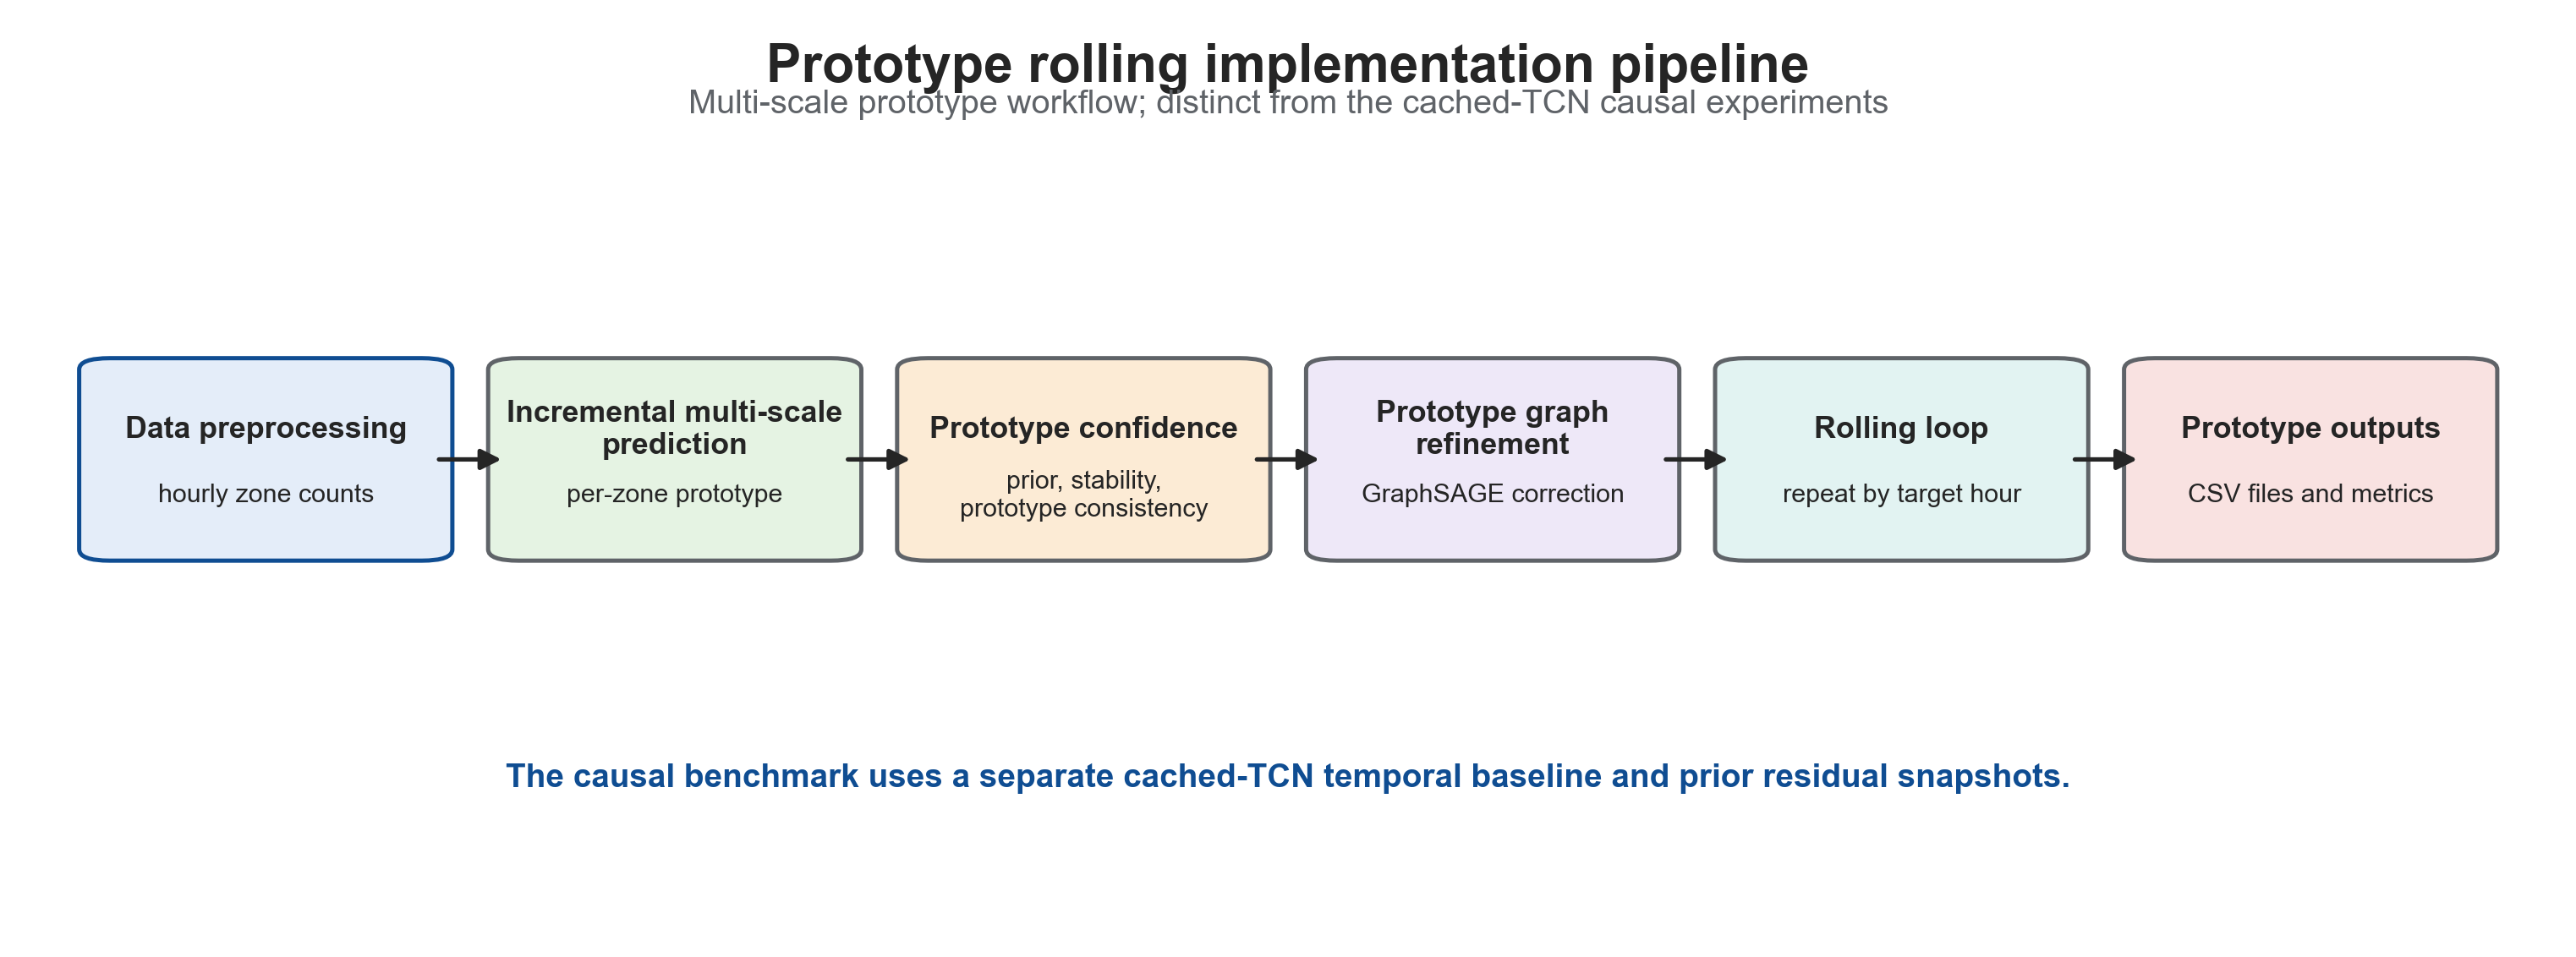
\includegraphics[width=1\textwidth]{img/4.3.png}
		\caption{Overall implementation pipeline for rolling taxi-demand prediction, combining data preprocessing, multi-scale temporal forecasting, confidence fusion, GraphSAGE refinement, and metric output generation.}
		\label{fig:4.3}
	\end{figure}
	
	The function \texttt{get\_true\_counts()} extracts the ground-truth count for a target hour by filtering the dataframe to the target timestamp and grouping by pickup location. This produces a mapping from \texttt{PULocationID} to observed demand. The rolling loop uses this mapping to assign \texttt{y\_true} for each zone. The implementation also builds \texttt{zone\_hourly\_counts}, a grouped pandas series over zone and hour, so that historical windows can be queried efficiently when constructing mean historical features.
	
	Historical mean features are computed in \texttt{\_compute\_history\_means()}. For each target hour and zone, the function creates three lookback windows corresponding to 24 hours, 168 hours, and 720 hours. The sum of observed hourly counts inside each window is divided by the window length, resulting in average demand over the short, weekly, and longer-term context. If a zone has no historical series, the feature dictionary defaults to zeros. These features are later passed into the graph pipeline and concatenated with the temporal prediction and confidence value.
	
	The temporal manager also performs its own internal preprocessing at the per-zone level. The function \texttt{\_prepare\_zone\_series()} constructs a dense hourly sequence for a single zone ending at the forecasting context end. It groups records by datetime, creates a full hourly date range, reindexes the grouped series to that range, fills missing hours with zero, and stores the result as floating-point passenger counts. This dense reconstruction is essential because a neural sequence model requires a regular input grid. Without explicitly inserting zero-demand hours, the model would not be able to distinguish inactivity from missing records.
	
	Scaling is implemented in \texttt{\_fit\_scaler\_hist()}. The scaler is fitted only on rows whose timestamps are earlier than the target hour, which helps preserve temporal integrity. The implementation also handles edge cases where the available history is empty, non-finite, or constant by fitting artificial two-point ranges. This avoids crashes in sparse zones and ensures that inverse scaling remains defined even when the historical range is degenerate.
	
	Training windows are constructed in \texttt{\_build\_training\_windows()}. The function uses the manager configuration to determine the sequence length and forecast horizon, scales the hourly counts, and then slides across the sequence to produce four input tensors: \texttt{1h}, \texttt{1d}, \texttt{1w}, and \texttt{1m}. The one-hour branch receives the most recent step, the daily branch receives the last 24 steps, the weekly branch receives the last 168 steps, and the monthly branch receives the full 720-step window. The target is the next-hour passenger count in scaled space. During inference, \texttt{\_build\_inference\_window()} uses the same duration mapping to build one aligned input dictionary ending at \texttt{context\_end}.
	
\section{Implemented Multi-Scale Temporal Candidate}
	
	The implemented temporal model combines recurrent and attention-based components in a single multi-scale architecture. The constructor defines LSTM encoders for the daily and weekly inputs, a linear projection followed by a Transformer for the monthly input, branch-level dropout layers, a linear feature-fusion layer, a GRU backbone, and a final fully connected output layer. This architecture directly implements the methodological choice that different time scales should be represented through specialised branches.
	
	
	\begin{figure}[h]
		\centering
		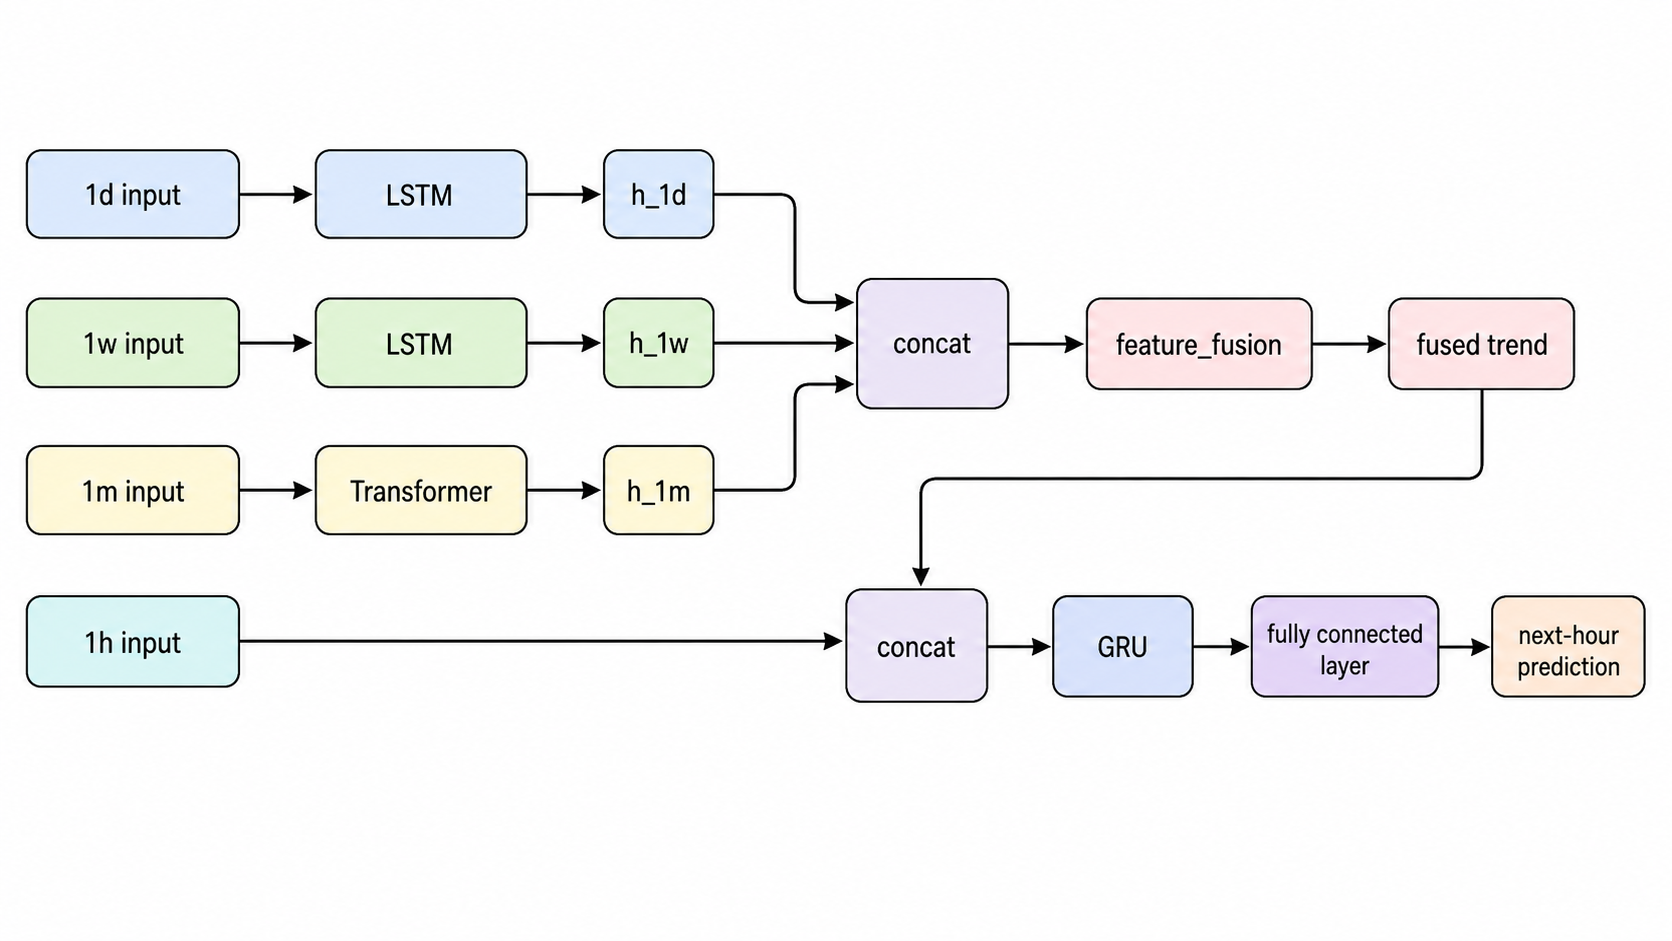
\includegraphics[width=1\textwidth]{img/4.4.png}
		\caption{Architecture of the multi-scale temporal predictor, where daily and weekly inputs are encoded by LSTM branches, the monthly input is encoded by a Transformer branch, and the fused trend representation is combined with the short-term input before GRU-based next-hour prediction.}
		\label{fig:4.4}
	\end{figure}
	
	During the forward pass, the model first encodes the daily, weekly, and monthly inputs. The daily and weekly branches return the final hidden states of their LSTM encoders. The monthly branch is projected from a scalar sequence into the hidden dimension and then passed through a Transformer; the final time step of the Transformer output is used as the monthly embedding. These three embeddings are concatenated and compressed through \texttt{feature\_fusion}. The fused trend representation is then repeated along the short sequence dimension and concatenated with the one-hour input to form the GRU input.
	
	This implementation makes the GRU a final prediction pathway rather than the only temporal encoder. The longer-term dynamics are represented before the GRU stage, and the GRU receives both immediate demand and the fused trend. This separation makes the model relatively interpretable: daily, weekly, and monthly context are encoded explicitly, while the final output head converts the fused information into a scalar next-hour prediction.
	
	Dropout is used in two ways. During normal training, it regularises the branch representations and the short-term hidden state. During uncertainty estimation, the model deliberately keeps dropout active through the \texttt{train()} mode inside the MC functions. In \texttt{mc\_predict()}, repeated stochastic forward passes produce a tensor of predictions, from which the mean and standard deviation are computed. In \texttt{mc\_branch\_embeddings()}, the same repeated-sampling idea is applied to hidden embeddings rather than only final predictions.
	
	Training is managed by \texttt{train\_once()}. If no checkpoint exists, the function prepares the dense zone series, builds training windows, creates a \texttt{MultiScaleModel}, and trains it with Adam and mean squared error. The loop tracks the best loss and uses a patience counter for early stopping. After training, the model, scaler, and metadata are saved. When the rolling context subsequently advances, the incremental manager performs a lightweight update instead of repeating full training.
	
	Inference is split into \texttt{predict()} and \texttt{predict\_with\_uncertainty()}. The plain prediction function loads the checkpoint, reconstructs the context end as one forecast horizon before the target date, prepares the dense series, fits the scaler on historical data before the target, builds the inference window, obtains the MC mean prediction, inverse-transforms it, and returns it as a float. The uncertainty function performs the same setup but additionally returns the original-scale predictive standard deviation and a dictionary of branch variances for the four temporal branches. This is the interface used by the rolling driver to populate \texttt{y\_pred}, \texttt{mc\_std}, and variance values for each zone.
	
	The orchestration method \texttt{train\_and\_predict\_if\_needed()} combines checkpointing, incremental updating, and forecasting. It computes the context end, trains the model if no checkpoint exists, loads metadata if a checkpoint does exist, and triggers \texttt{incremental\_update()} when the stored context is older than the current context. It then returns the prediction for the target date.
	
\section{Confidence Implementation in the Causal Experiments}
	
The causal experiment runners construct confidence from three components: a prior score based on pickup volume before the target hour, a stability score based on MC Dropout variance, and a historical-consistency score derived from 24-hour, 168-hour, and 720-hour mean demand. The cached TCN detail file supplies available confidence components; the runner recomputes missing historical-consistency values from causal look-back summaries.
	
	
	\begin{figure}[h]
		\centering
		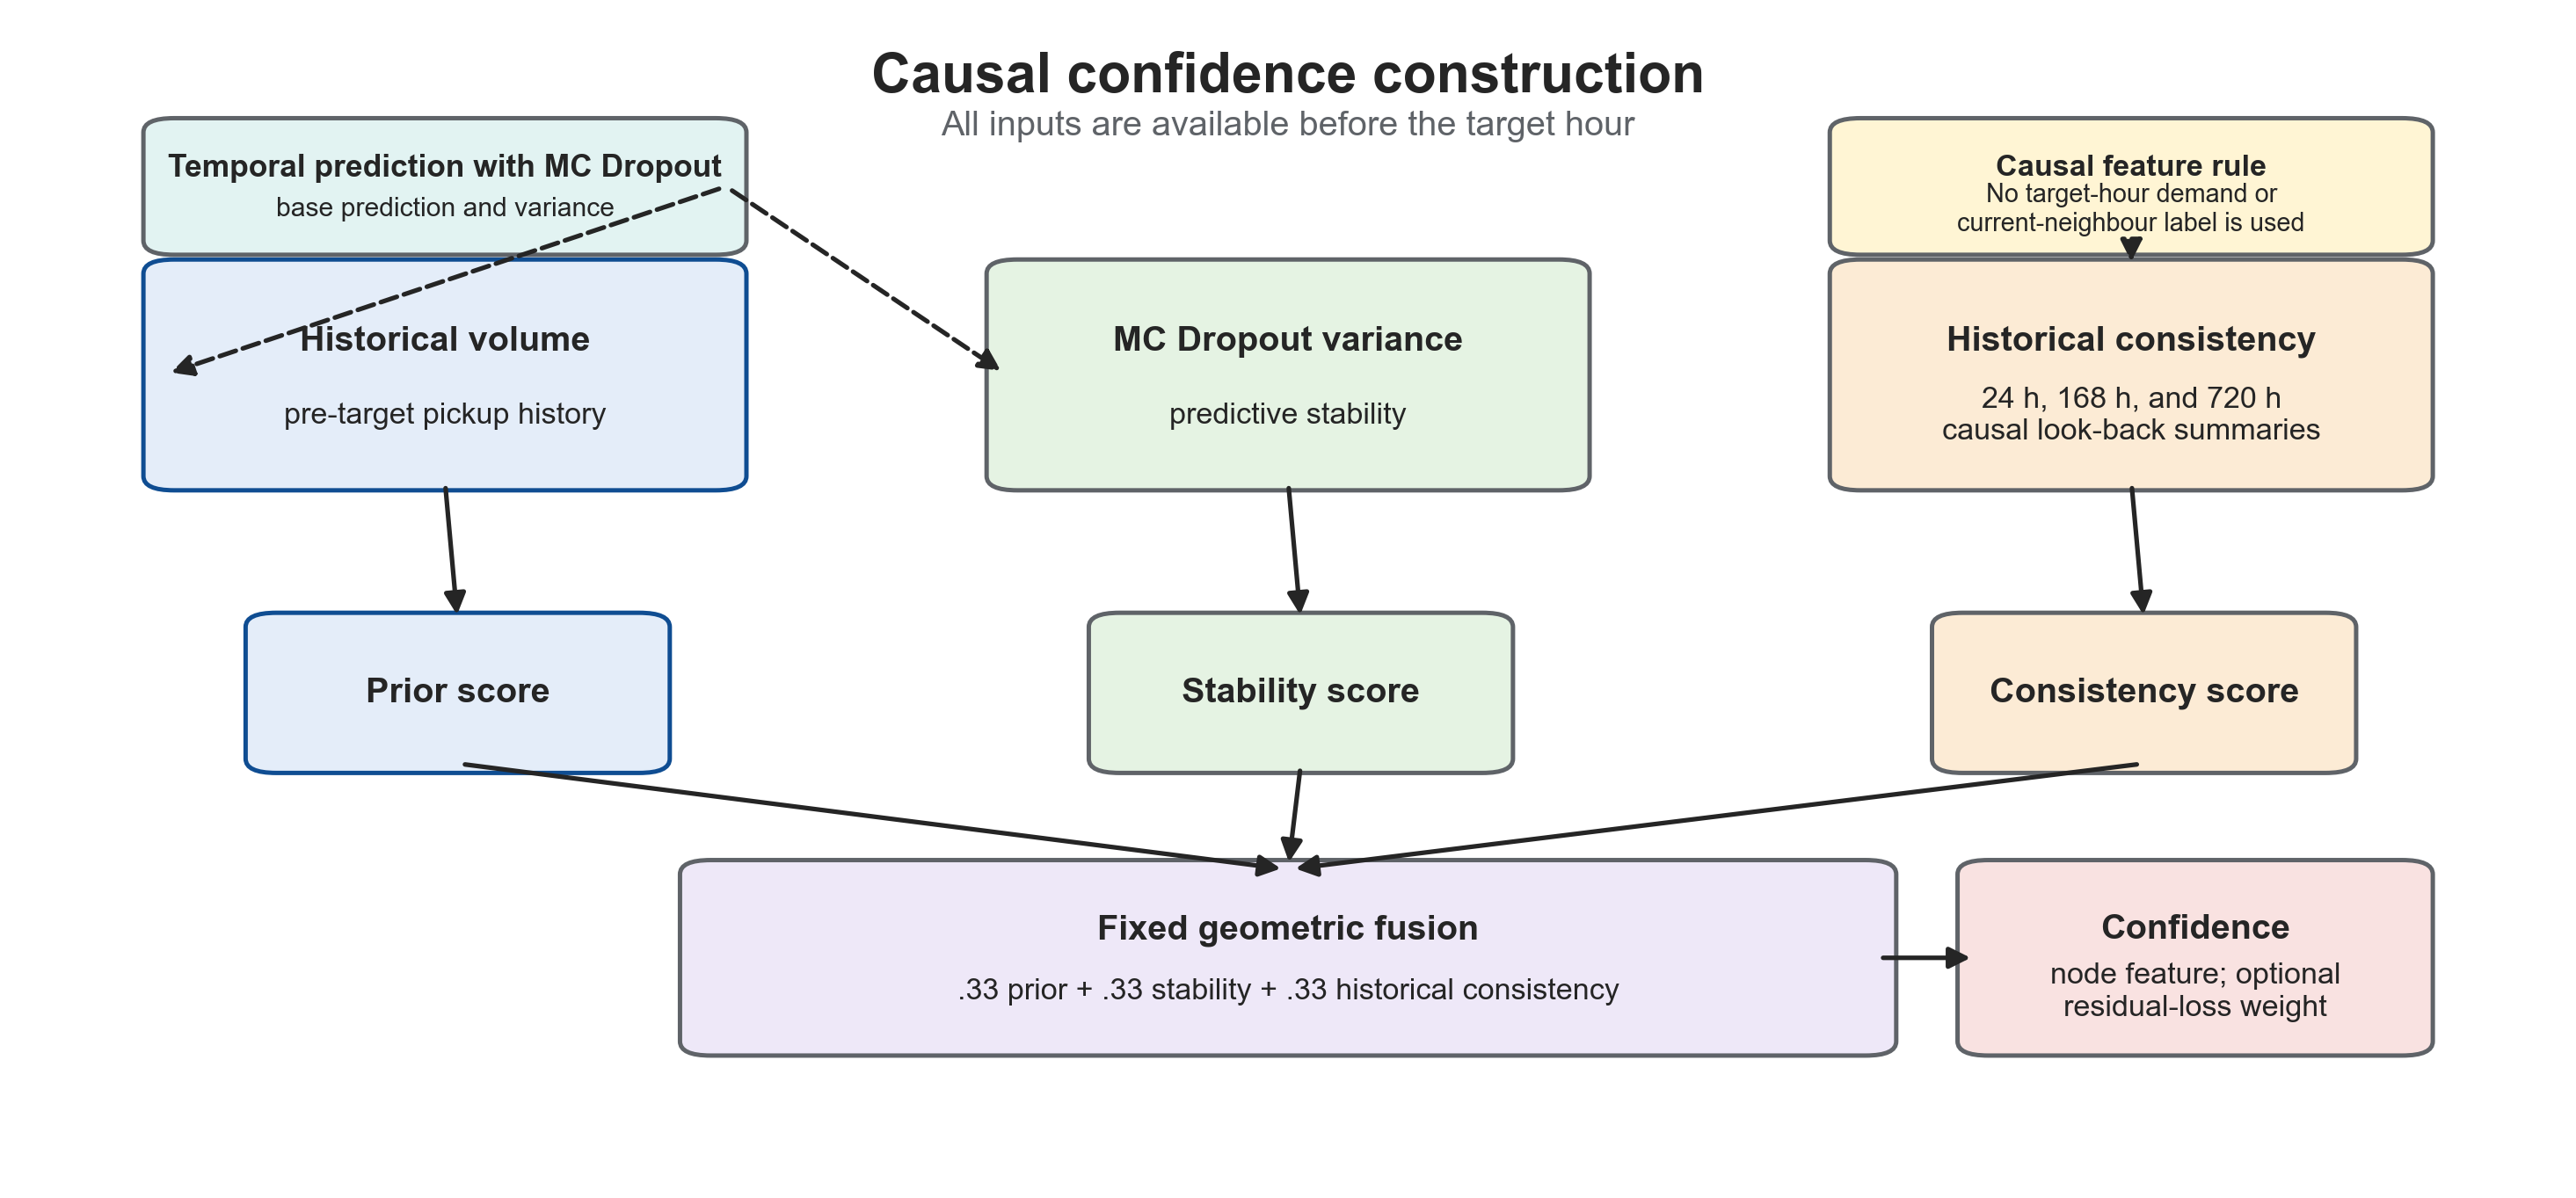
\includegraphics[width=1\textwidth]{img/4.5.png}
\caption{Confidence fusion mechanism combining historical prior, MC Dropout-based stability, and historical consistency into a zone-level reliability score. In the causal experiments it is available as a node feature and, in the confidence ablations, as a residual-loss weight.}
		\label{fig:4.5}
	\end{figure}
	
For each target hour, the prior uses only preceding observations. The runner sums pre-target zone counts, applies \(\log(1+x)\), min--max normalises across eligible zones, and rescales the result to \([0.2,1]\). Zones with richer historical support therefore receive a larger prior score without using target-hour demand.
	
The stability score is computed at every rolling step from the available MC variance. The implementation uses the median finite variance as a scale parameter and applies an exponential decay, so predictions with larger variance receive lower stability scores.
	
The historical-consistency score is also computed at every rolling step. For each zone, the runner takes the log-transformed 24-hour, 168-hour, and 720-hour demand means, calculates their dispersion, and maps it through a clipped exponential decay. Agreement across the three causal histories yields a higher score.
	
The fusion function clips all three components into a safe interval and combines them in log space, corresponding to a weighted geometric mean. The fixed comparator in the weight-sensitivity experiment uses equal prior, stability, and historical-consistency weights of \(0.33,0.33,0.33\). The experiments then compare component ablations and alternative fusion-weight selection methods. The resulting score is stored in each step dataframe and used as a node feature in the causal residual GNN.
	
\section{Causal Graph Refinement Implementation}
	
Each causal runner begins with cached no-graph TCN predictions. For a target hour, it creates the current inference snapshot containing \texttt{base\_pred}, confidence, historical features, and the observed value retained only for final metrics. It then selects residual snapshots strictly earlier than the target hour, using the matching peak or non-peak partition, and concatenates those snapshots into the graph-training data.
	
	\begin{figure}[h]
		\centering
		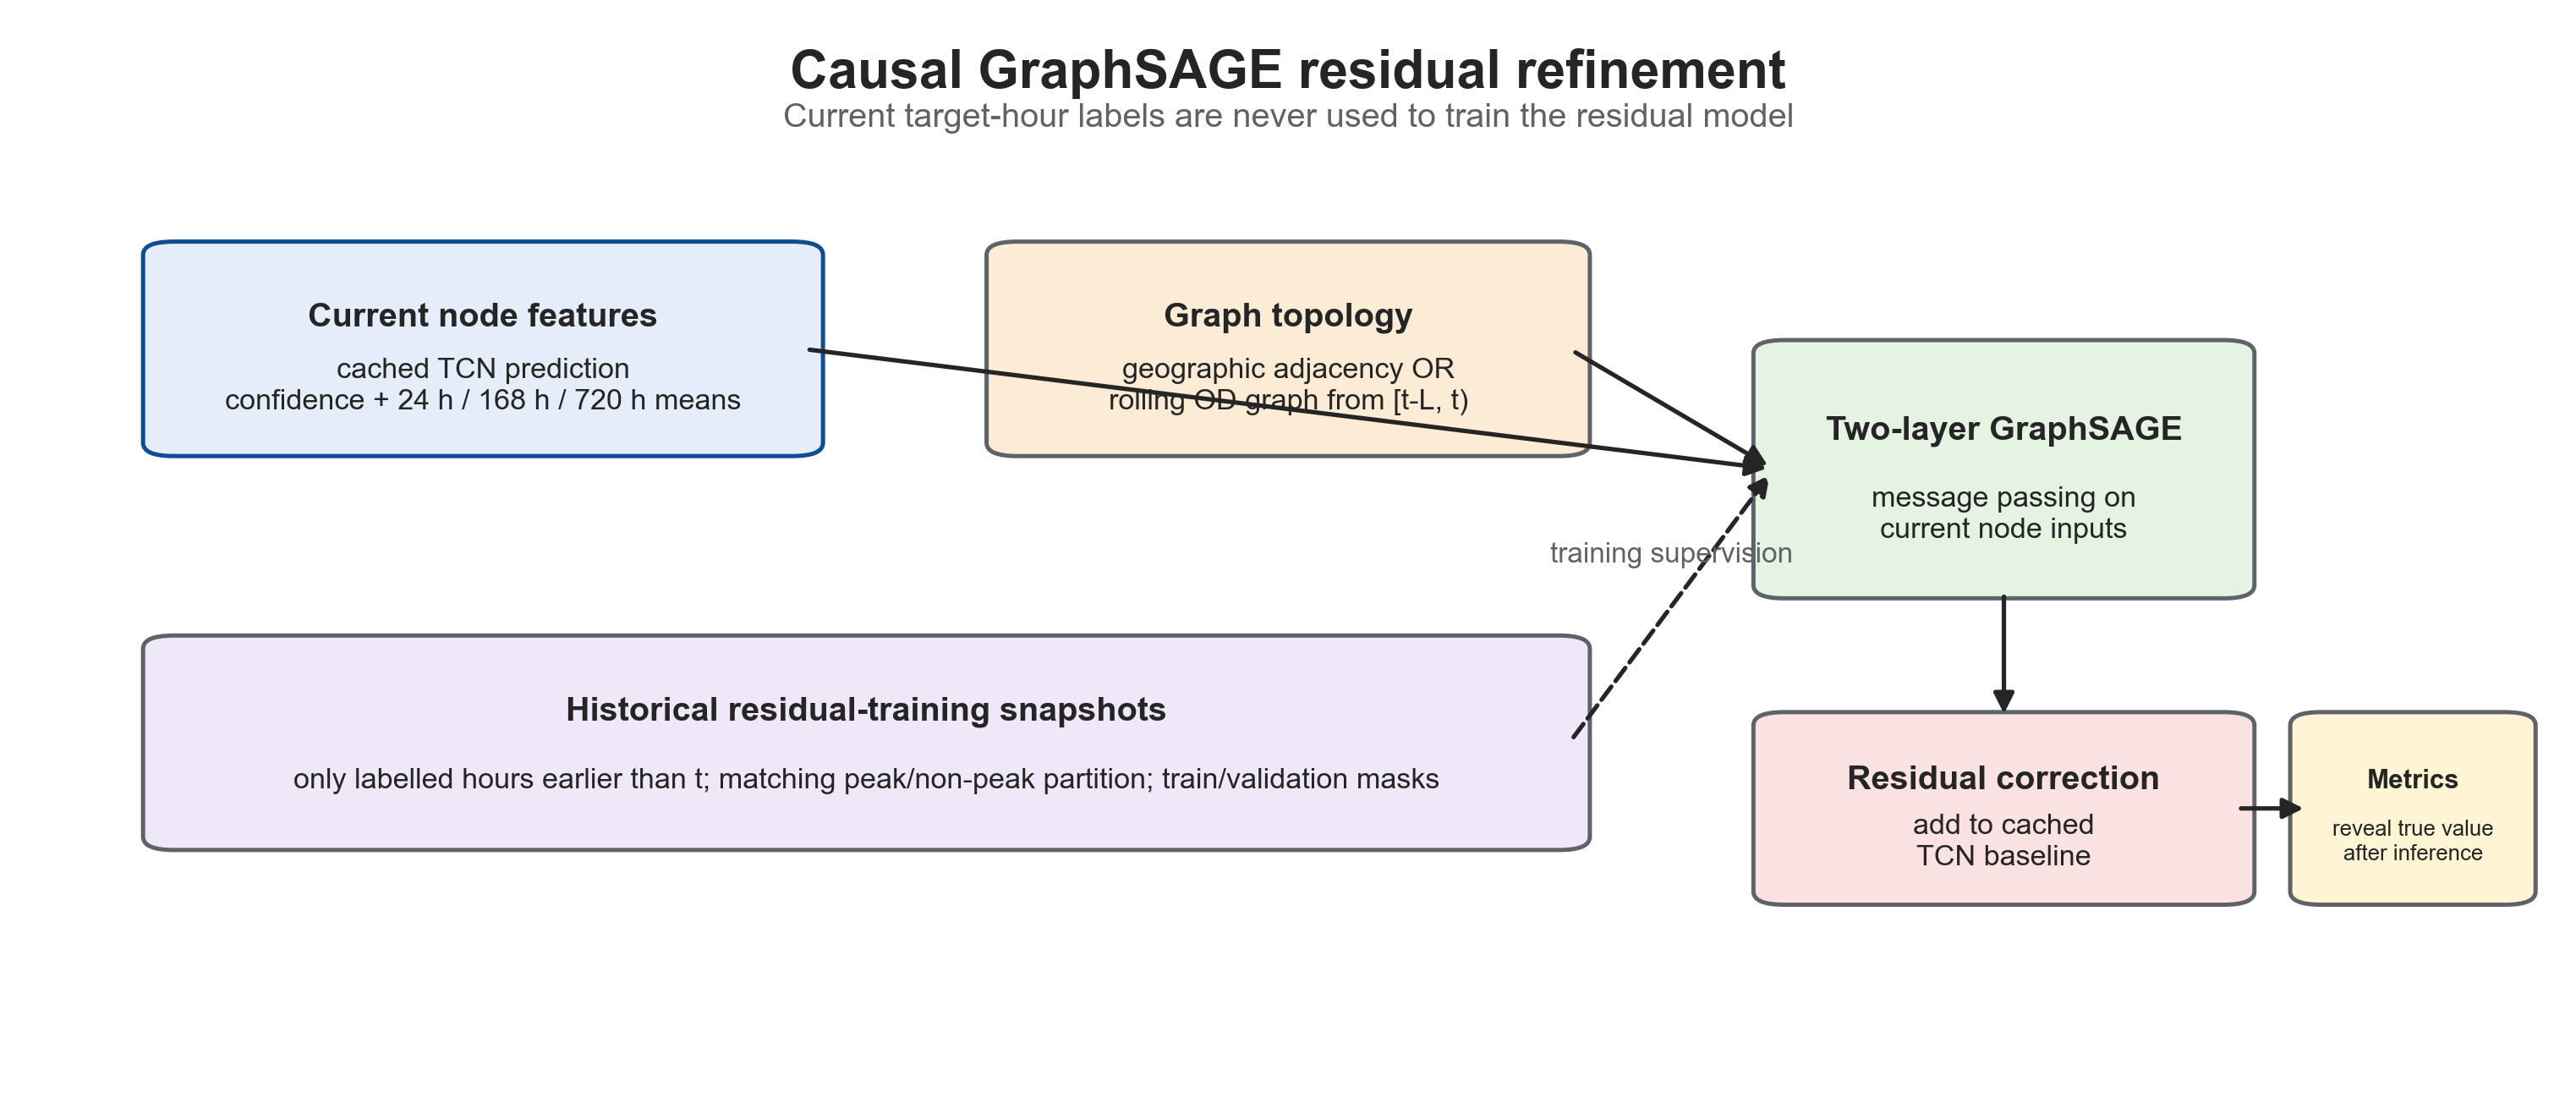
\includegraphics[width=1\textwidth]{img/4.6.png}
\caption{Causal GraphSAGE residual refinement. Cached TCN predictions, confidence scores, and historical means form node inputs. Geographic or rolling OD graph topologies define message passing, while only earlier labelled snapshots form residual-training targets.}
		\label{fig:4.6}
	\end{figure}
	
For rolling OD variants, the runner constructs an OD matrix from trips in \([t-L,t)\), retains the top destinations for each origin, and saves the resulting matrix for the target hour. Geographic and rolling OD matrices are converted into sparse edge indices that define the neighbourhood used by the graph model.
	
The node feature vector comprises the cached TCN prediction, full confidence, and the three historical means. The graph model is a two-layer mean-aggregation GraphSAGE network with GELU activations and dropout. The residual target is \texttt{true\_value - base\_pred}; the target-hour value is not used in the graph-training snapshots.
	
Eligible locations are assigned once to 60\% training, 20\% validation, and 20\% test partitions using fixed seed 42; the same partitions are reused throughout the rolling evaluation. Training and validation masks are applied only to the concatenated historical snapshots; the current snapshot uses the test mask for reporting. The model uses dropout 0.1, hidden dimension 256, Adam, cosine annealing, Smooth \(L_1\) loss, and up to 300 epochs with patience 40. Confidence weighting is varied only in the dedicated confidence experiments; the graph-topology experiment uses an unweighted residual loss.
	
\section{Causal Experiment Runners}
	
The causal runners share a common rolling structure. \texttt{demo\_test.py} evaluates the eight temporal backbones in Experiment~1 and imports \texttt{persistent\_multiscale\_incre\_confi.py} when the multi-scale candidate is selected. Experiments~2--6 reuse cached no-graph TCN predictions, so the residual studies do not retrain the temporal baseline or invoke a multi-scale manager. Each runner writes detailed per-zone predictions, hourly summaries, and aggregate metrics to a dedicated result directory.
	
	\begin{figure}[h]
		\centering
		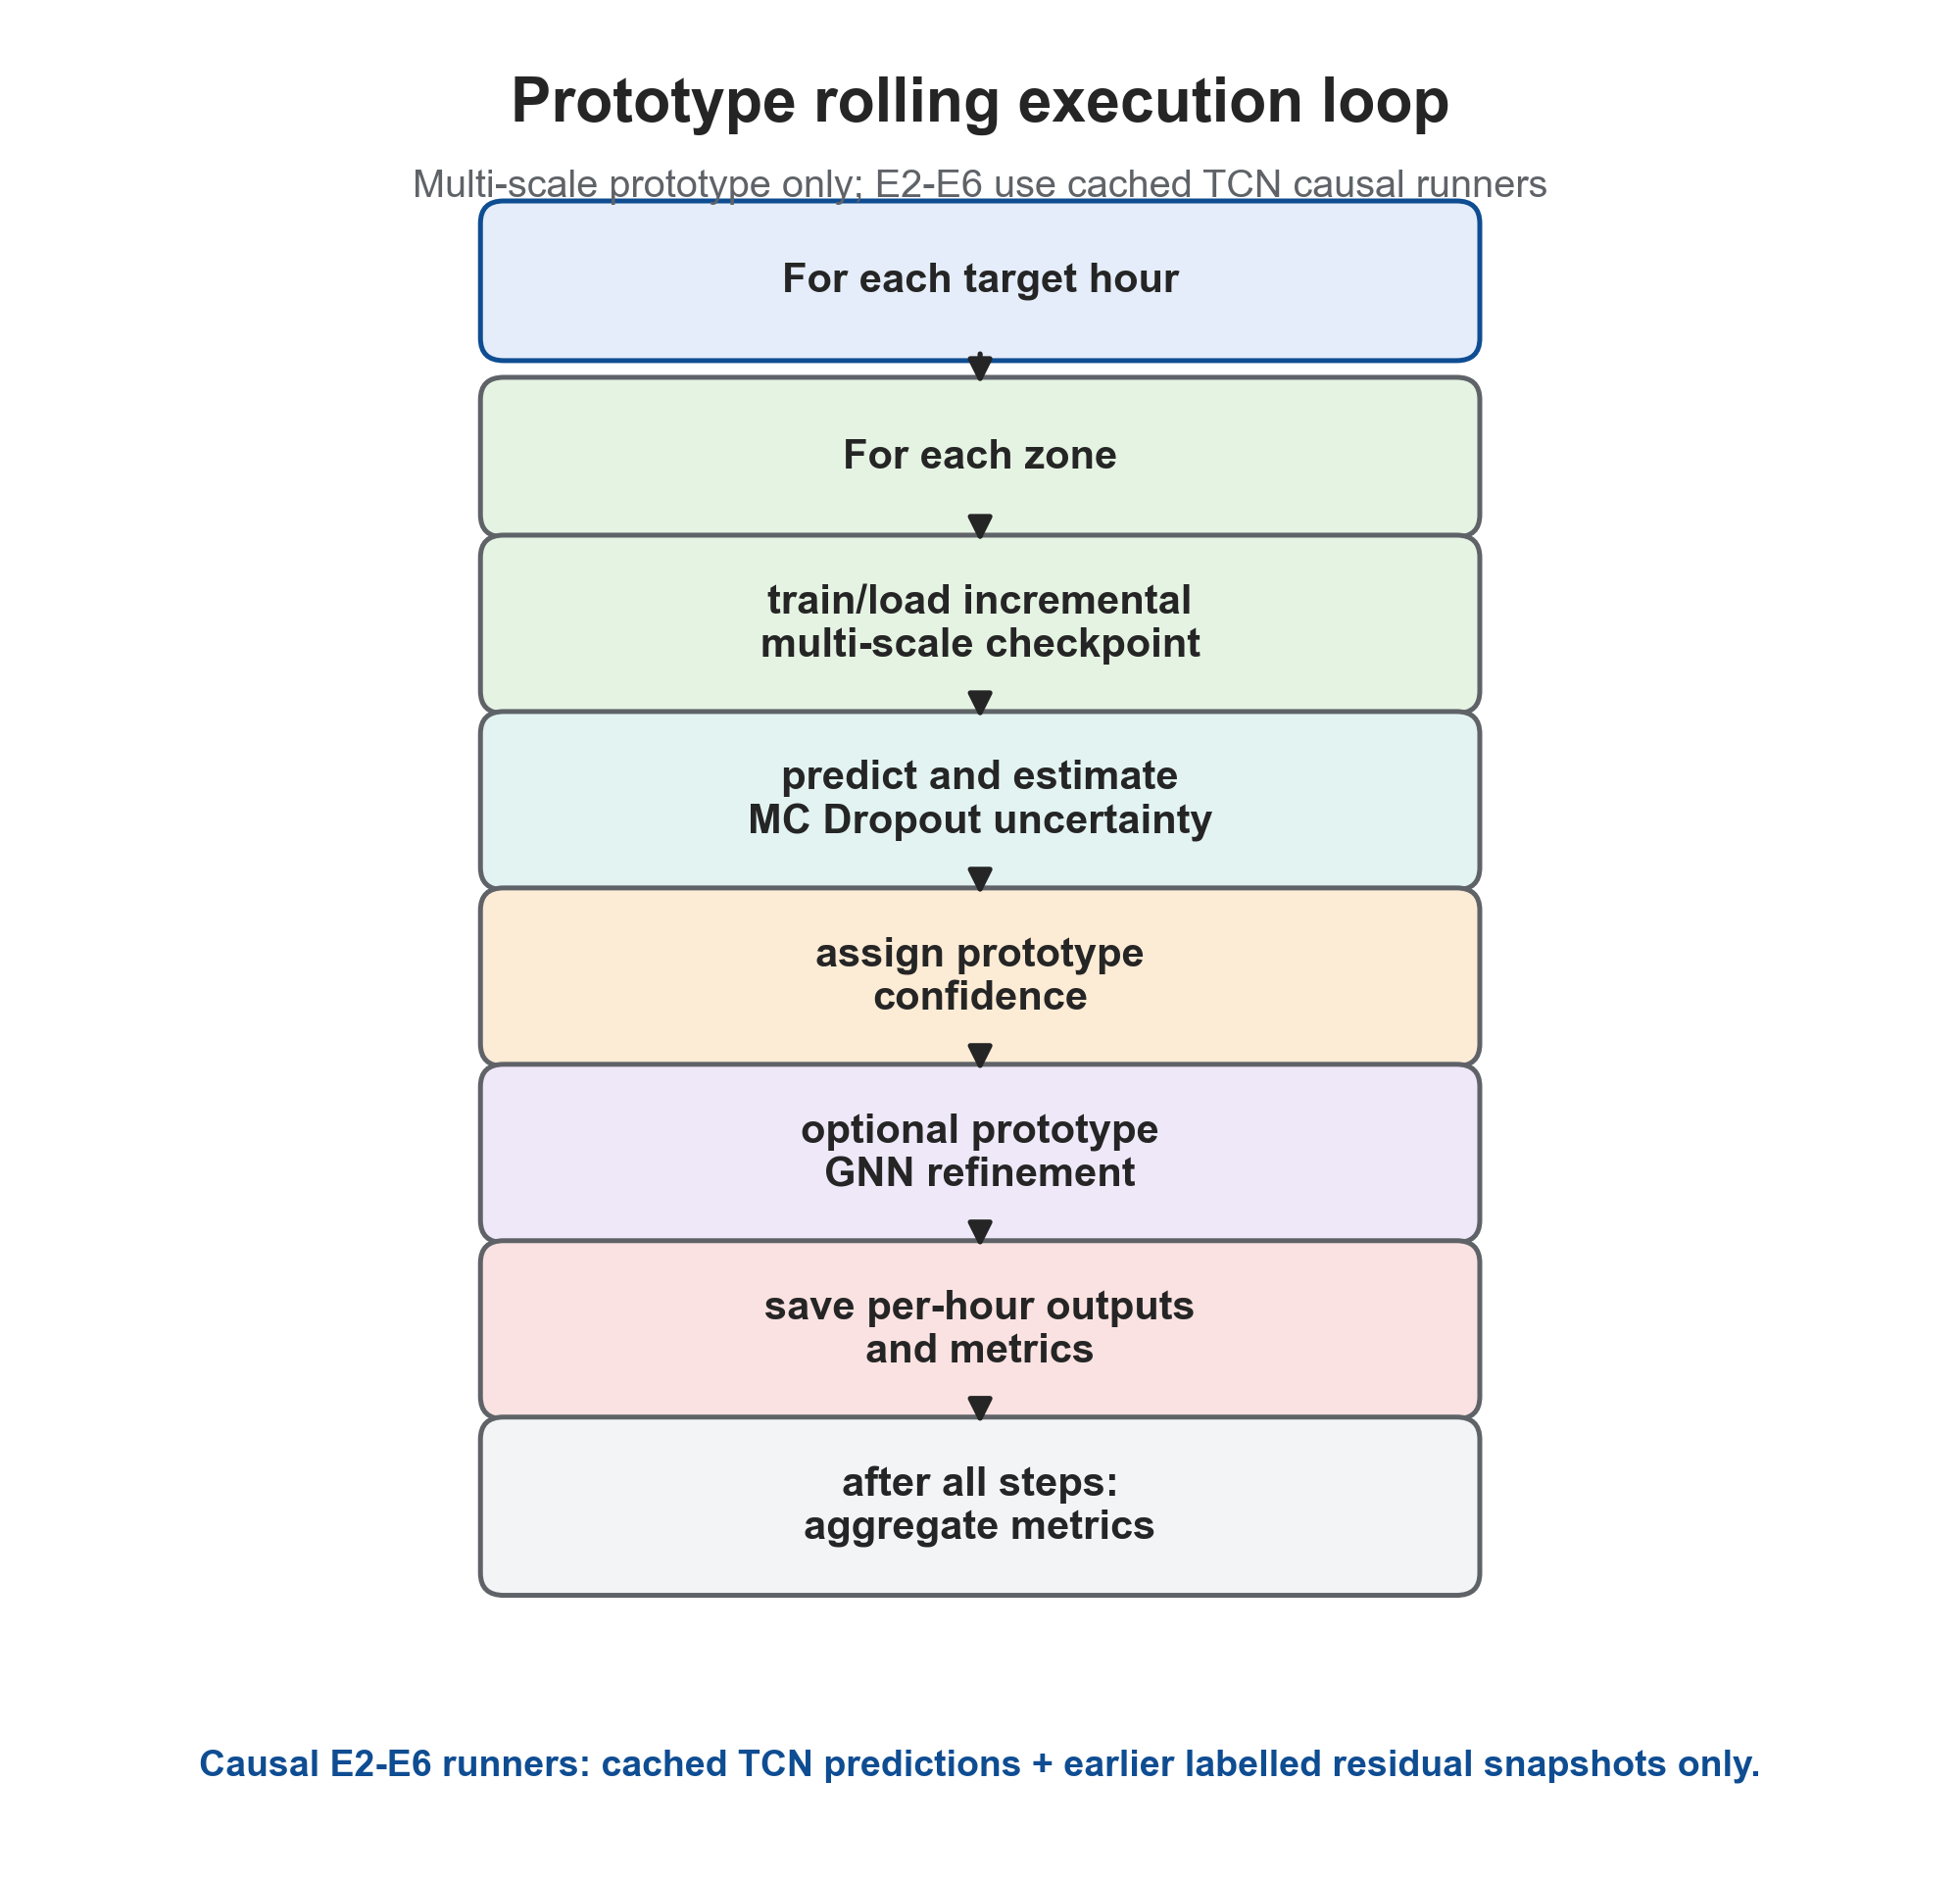
\includegraphics[width=1\textwidth]{img/4.7.png}
		\caption{Rolling execution loop for hourly taxi-demand prediction, uncertainty estimation, confidence assignment, GraphSAGE refinement, and final metric aggregation.}
		\label{fig:4.7}
	\end{figure}
	
	
Within each 24-hour window, causal residual history is local to that window. The code retains only snapshots whose label hour precedes the current target. With the peak/non-peak split, the initial non-peak hour and the first peak hour in a window have no matching historical residual snapshot. In those cases, the residual model falls back to the TCN base prediction. Experiment~2 also provides a summary excluding the first target step of each window; the active-refinement graph comparison excludes all target hours without a matching historical snapshot.
	
	\section{Checkpoint and Incremental-Update Handling}
	
	Checkpointing is implemented in the temporal manager. For each zone, the model path, scaler path, and metadata path are generated from the checkpoint directory and zone identifier. The manager considers a zone to have a checkpoint only when both model and scaler files exist. This avoids loading a partial checkpoint where the neural model exists but the scaler is missing, or vice versa.
	
	The project uses the incremental manager in \path{code/persistent_multiscale_incre_confi.py}. If no valid checkpoint exists, the manager performs full training. If a checkpoint exists but its stored context end is older than the current context, it triggers a lightweight \texttt{incremental\_update} before prediction. The updated model, scaler, and metadata are saved again.
	
	Both \texttt{demo\_rolling\_GNN.py} and the multi-scale candidate in \texttt{demo\_test.py} use this manager. Experiments~2--6 instead reuse cached TCN forecasts and do not execute a multi-scale manager.
	
	This configuration is the only multi-scale configuration reported in the thesis. Experiments~2--6 use cached TCN forecasts, so their temporal-model behaviour is distinct from the incremental multi-scale benchmark.
	
	
	\section{Incremental Multi-Scale Manager}
	
	The sole multi-scale implementation is \path{persistent_multiscale_incre_confi.py}. It uses four temporal branches, branch-level dropout, multi-scale fusion, a GRU-based prediction pathway, and a Monte Carlo Dropout uncertainty interface. Its manager logic adds lightweight incremental updating after the first full training run, reducing the instability that can occur when a fixed checkpoint is reused over a long rolling horizon while new observations continue to arrive.
	
	Structurally, the incremental version still uses the same \texttt{MultiScaleModel} class design. The model contains LSTM encoders for the 1-day and 1-week branches, a Transformer-based encoder for the 1-month branch, dropout layers for Monte Carlo sampling, a fusion layer for combining longer-term temporal representations, and a GRU pathway for producing the final next-hour prediction. It also retains the Monte Carlo interfaces for repeated stochastic prediction and branch-embedding variance estimation. Therefore, the incremental version should not be understood as a different forecasting architecture. Rather, it is a different training and model-management strategy built around the same multi-scale temporal backbone.
	
	The configuration and orchestration logic include \texttt{epochs\_incremental}, \texttt{lr\_incremental}, \texttt{weight\_decay}, and \texttt{grad\_clip}. These parameters separate full initial training from subsequent lightweight adaptation. Full training is used when no checkpoint exists. Incremental training is deliberately small: it updates an existing model with newly available rolling-window observations rather than rebuilding the model from the beginning.
	
	The core extension is the \texttt{incremental\_update} routine. When the manager detects that the previous training context is older than the new forecasting context, it loads the existing checkpointed model and performs a short additional optimisation step over newly arrived hourly samples. The update interval is defined by the gap between \texttt{prev\_until} and \texttt{new\_until}. Instead of reconstructing the entire historical training process, the function builds incremental windows only for the newly available timestamps in this interval. This design makes the update computationally cheaper than full retraining while still allowing the model parameters to respond to recent observations.
	
	The incremental update procedure also refits the scaler using recent historical data before applying the update. In the provided implementation, this recent fitting range is based on the final 30 days before the new context end. The dense hourly series is rebuilt up to \texttt{new\_until}, the scaler is fitted on recent history, the newly available training windows are assembled, and the existing model is fine-tuned using a Smooth L1 loss. The use of Smooth L1 loss in the incremental stage is appropriate because rolling updates may be exposed to local spikes or sparse-zone irregularities, and Smooth L1 is less sensitive to extreme residuals than pure squared error.
	
	Another important detail is that the incremental version applies gradient clipping during fine-tuning. This prevents a small number of recent windows from producing excessively large parameter updates. In the context of online or semi-online forecasting, this is a practical safeguard: the purpose of incremental learning is to stabilise the model under gradual drift, not to let a single short update overwrite the previously learned temporal structure. The addition of weight decay also regularises the update and further reduces the risk of overfitting to the newest observations.
	
	During full training and incremental updating, the model can collect branch embeddings under Monte Carlo Dropout and derive confidence-style weights from the variance of those embeddings. In the current code, the auxiliary-head structure is declared in the model, and branch-confidence quantities are computed. However, the auxiliary loss contribution is effectively neutralised because the auxiliary term is multiplied by zero before being added to the main loss. Therefore, the thesis should describe this part carefully: the incremental manager contains the architectural and computational hooks for confidence-weighted auxiliary learning, but the active optimisation objective is currently dominated by the main prediction loss.
	
	The orchestration logic is explicit. If a checkpoint already exists and its metadata is older than the current context, the manager triggers \texttt{incremental\_update}. After updating, the model, scaler, and metadata are saved again, and the new metadata records the updated context end. The manager therefore maintains a moving checkpoint state that follows the rolling prediction horizon.
	
	From an implementation perspective, the manager interface, especially \texttt{train\_and\_predict\_if\_needed} and \texttt{predict\_with\_uncertainty}, keeps the update mechanism isolated from the rest of the rolling pipeline. The temporal model-management behaviour can therefore adapt to the advancing context without changing the multi-scale architecture or the graph-refinement interface.
	
	In this thesis, \path{persistent_multiscale_incre_confi.py} is the only reported multi-scale configuration. It is evaluated for the Experiment~1 multi-scale candidate and allows newly observed time windows to update the temporal model. Experiments~2--6 use cached TCN forecasts rather than a multi-scale manager. This distinction is important for reproducibility because the temporal benchmark and the causal residual experiments have different temporal-model behaviour.
	
	\section{Output Artefacts and Evaluation Files}
	
	The implementation produces several categories of output artefacts. The first category consists of temporal baseline outputs. \texttt{predictions\_rolling\_mc.csv} contains per-zone rolling records including prediction, true value, uncertainty, variance, error status, historical mean features, confidence, and target hour. \texttt{hourly\_metrics\_gru.csv} contains per-hour baseline MAE, RMSE, and mean true demand. These files are generated in the rolling driver after all rolling steps are complete.
	
	The second category consists of graph-refinement outputs. For each target hour, \texttt{run\_gnn\_pipeline()} can write a single-hour CSV named according to the target timestamp. This file includes \texttt{PULocationID}, \texttt{ZoneName}, \texttt{GRU\_Pred}, \texttt{Refined\_Pred}, \texttt{True\_Value}, and \texttt{Confidence}. Across all rolling steps, the driver writes \texttt{gnn\_refined\_predictions.csv}, which aggregates graph-refined rows over time, and \texttt{hourly\_metrics\_gnn.csv}, which stores per-hour MAE and MSE for both baseline and graph-refined predictions.
	
	The third category is the summary metric file. The driver computes overall baseline MAE/RMSE from all valid baseline rows and overall graph MAE/RMSE from all valid graph-refined rows, then writes these values into \texttt{overall\_metrics\_gnn.txt}. This gives a compact experiment summary, while the CSV outputs preserve sufficient detail for later plotting, error analysis, and ablation comparisons.
	
	The graph module also supports optional visual diagnostics. If plotting is enabled, it produces bar charts comparing MAE and MSE between baseline and graph-refined predictions, and a scatter plot comparing true values with both GRU and GNN predictions. In the rolling driver, plotting is disabled during automated execution to avoid interrupting batch runs.
	
\section{Implementation-Level Limitations}

The causal runners avoid target-hour residual supervision, but they retain several implementation limits. First, graph-training histories are reset at the start of every 24-hour window. The first prediction step has no residual history and therefore receives the uncorrected TCN prediction. Second, the location-based partitions do not establish a temporally disjoint month-to-month hold-out cohort over the full horizon.

Third, the reported graph comparison uses alternative geographic and OD topologies under mean aggregation. Confidence is not used as an edge weight; it is a node feature and, in selected experiments, a sample-weighting signal. Fourth, the per-zone temporal implementation used in Experiment~1 increases the number of checkpoints and would need more systematic experiment tracking in a larger deployment.
	
	Fourth, the incremental manager updates a separate checkpoint for each zone as the rolling context advances. This increases the number of checkpoint states and would require more systematic experiment tracking in a larger deployment. Experiments~2--6 reuse cached TCN forecasts and therefore do not share this update behaviour.
	
	\section{Summary}
	
In implementation terms, the project is a modular rolling forecasting system. The Experiment~1 runner evaluates per-zone temporal candidates and uses the incremental manager for the multi-scale implementation. The causal runners reuse cached TCN predictions, compute confidence and historical features, build geographic or rolling OD graphs, train GraphSAGE models on earlier residual snapshots, and write per-zone and aggregate outputs.
	
The codebase is not a single isolated model script. It provides explicit data preparation, temporal prediction, confidence fusion, graph refinement, rolling evaluation, and reproducible outputs. It also makes the boundary between the legacy prototype and the causal experiment runners explicit. The latter, rather than the same-hour prototype path, determine how the results in the following chapter should be interpreted.
	
	% ---------------------------
	% Chapter 5: Experiments
	% ---------------------------
	\chapter{Experiments}
	\label{chap:experiments}
	
	\section{Experimental Objectives}
	
	This chapter evaluates the temporal-first residual framework under a causal rolling protocol. The temporal model first produces zone-level next-hour forecasts from observations before the target hour. GraphSAGE subsequently learns residual corrections from historical labelled residual snapshots; it does not use target-hour labels for training. This separation is essential: the graph stage is evaluated as a forecasting correction mechanism rather than as within-hour interpolation.
	
The experiments address six questions: (i) which temporal backbone is suitable for the residual pipeline; (ii) whether residual node features improve correction; (iii) which graph topology helps; (iv) whether confidence-derived sample weighting helps; (v) how sensitive the confidence fusion weights are; and (vi) whether confidence is associated with realised error. The multi-scale model developed in this thesis is evaluated under the same twelve-window protocol as the other temporal backbones, enabling a direct comparison with TCN.
	
	\section{Dataset and Causal Preprocessing}
	
	The experiments use NYC taxi trip records aggregated into hourly pickup counts by Taxi Zone. Each trip contributes one pickup to its pickup hour and zone, yielding a dense zone-hour demand matrix after zero filling. Zones with unstable or non-standard identifiers (46, 103, 104, 105, 264, and 265) are excluded before temporal modelling, graph construction, and evaluation. The remaining 259 graph-compatible zones are used consistently in the causal benchmark.
	
	All temporal inputs use observations strictly before the target hour. Historical summary features are computed over 24-hour, 168-hour, and 720-hour look-back windows. For a target hour $t$, a rolling OD graph with look-back length $L$ contains trips in $[t-L,t)$ only and retains the top outgoing destinations for each origin. Therefore, neither target-hour pickup counts nor target-hour trips are used to construct a graph for that prediction.
	
	\section{Evaluation Protocol}
	\label{sec:causal-evaluation-protocol}
	
The cached-temporal benchmark uses twelve 24-hour rolling windows across March--December 2021, giving 288 target hours. The temporal-backbone study contains $12\times24\times259=74{,}592$ zone-hour predictions per causal backbone. For each target hour, the temporal forecast and confidence components are generated first. The residual GraphSAGE model is then trained only on labelled snapshots earlier than the target hour and is evaluated on the current graph. Where applicable, the fixed seed 42 location cohort split assigns 60\% of eligible locations to training, 20\% to validation, and 20\% to test; these partitions are reused across target hours.
	
For residual learning, peak hours are 06:00--09:00 and 16:00--18:00. Historical snapshots are partitioned by peak status and each target hour uses the corresponding earlier partition. In the reported conference-style summaries, Experiments~2, 4, and~5 exclude the deterministic first prediction step of each rolling window. Experiment~3 reports active-refinement graph-valid predictions. In the feature, confidence-weighting, and reliability experiments, residual predictions at peak hours are multiplied by 0.3 before being added to the base forecast. This shrinkage is not used in the graph-topology experiment, which uses an unweighted residual loss and treats confidence as a node feature.
	
	MAE is the primary metric because zone-level pickup demand is sparse and heavy-tailed. RMSE and MSE quantify larger errors, and the standard deviation of hourly MAE describes rolling variability. The Experiment~3 improvement column follows the conference reporting convention: its percentages are calculated against the Experiment~2 first-step-excluded temporal baseline (MAE 19.87), although Experiment~3 absolute errors are reported on the active-refinement graph-valid population. The percentage is therefore a descriptive reference comparison rather than a matched-population effect estimate.
	
	\begin{table}[H]
	    \centering
	    \caption{Causal experiment roadmap.}
	    \label{tab:causal-roadmap}
	    \small
	    \begin{tabular}{p{0.13\linewidth}p{0.29\linewidth}p{0.27\linewidth}p{0.21\linewidth}}
	        \toprule
	        Experiment & Question & Main variable & Evaluation scope \\
	        \midrule
	        E1 & Which causal backbone? & Temporal model & 74,592 zone-hours \\
	        E2 & Do residual features help? & Node features & 14,076; no step 0 \\
        E3 & Which graph helps? & Graph topology & 13,679--13,728 active predictions \\
        E4 & Does confidence weighting help? & Sample-weight mode & 14,076; no step 0 \\
        E5 & Are fusion weights sensitive? & Fusion-weight selection & 14,076; no step 0 \\
	        E6 & Does confidence reflect error? & Confidence group & 14,688 test predictions \\
	        \bottomrule
	    \end{tabular}
	\end{table}
	
	\section{Experiment 1: Temporal Model Comparison}
	\label{sec:temporal-model-comparison}
	
	Table~\ref{tab:causal-temporal-backbone} compares the temporal backbones evaluated under the common twelve-window causal protocol. TCN has the lowest MAE and RMSE and is therefore the backbone used to produce the cached forecasts for Experiments~2--6. The re-run multi-scale model is close to TCN, but remains higher by 0.34 MAE (1.68\%), 1.03 RMSE, and 70.24 MSE. DLinear and PatchTST were obtained from a dedicated rerun summary; the remaining causal baselines were evaluated in the same overall comparison.
	
	\begin{table}[H]
	    \centering
	    \caption{Temporal-backbone comparison over twelve causal rolling windows. Lower is better.}
	    \label{tab:causal-temporal-backbone}
	    \resizebox{\textwidth}{!}{%
	    \begin{tabular}{lrrr}
	        \toprule
	        Temporal model & MAE & RMSE & MSE \\
	        \midrule
	        SARIMA & 73.32 & 145.53 & 21177.90 \\
	        DLinear & 31.04 & 54.86 & 3010.00 \\
	        GRU & 27.62 & 45.46 & 2066.90 \\
	        LSTM & 26.79 & 45.37 & 2058.20 \\
	        PatchTST & 26.38 & 45.18 & 2041.15 \\
	        Transformer & 21.80 & 37.47 & 1404.37 \\
	        \textbf{TCN} & \textbf{20.19} & \textbf{33.49} & \textbf{1121.56} \\
	        Multi-scale & 20.53 & 34.52 & 1191.80 \\
	        \bottomrule
	    \end{tabular}}
	\end{table}
	
	\section{Experiment 2: Residual Refinement Feature Ablation}
	
	The core GraphSAGE model predicts the residual $y_{i,t}-\hat{y}^{(T)}_{i,t}$ rather than demand from scratch. Table~\ref{tab:causal-feature-ablation} tests which causal node features support this correction. The base temporal forecast alone already supports an improvement over the cached temporal baseline. Confidence provides a small additional gain, while historical summary features provide the larger improvement in this run. The combination of confidence and history features gives the best MAE.
	
	\begin{table}[H]
	    \centering
	    \caption{Causal residual feature ablation after excluding the first prediction step of each rolling window.}
	    \label{tab:causal-feature-ablation}
	    \resizebox{\textwidth}{!}{%
	    \begin{tabular}{lrrr}
	        \toprule
	        Method & MAE & RMSE & MAE improvement \\
	        \midrule
	        Temporal baseline & 19.87 & 33.07 & -- \\
	        Base feature residual GNN & 18.33 & 32.85 & 7.73\% \\
	        Base + confidence feature residual GNN & 18.29 & 32.69 & 7.93\% \\
	        Base + history feature residual GNN & 17.72 & 31.61 & 10.82\% \\
	        \textbf{Base + confidence + history residual GNN} & \textbf{17.67} & 31.66 & \textbf{11.05\%} \\
	        \bottomrule
	    \end{tabular}}
	\end{table}
	
	\section{Experiment 3: Graph Structure Comparison}
	
This experiment compares graph topology while holding node features, causal residual history, and the unweighted residual loss fixed. Geographic adjacency and causal rolling OD graphs all improve over the no-graph temporal baseline on active-refinement predictions. The 60-day OD graph is marginally best at full precision, but its advantage over geographic adjacency is small. The defensible conclusion is that both functional flow and spatial proximity provide useful residual structure; the experiment does not establish a material advantage for OD topology.
	
	\begin{table}[H]
	    \centering
\caption{Graph structure comparison on active-refinement graph-valid predictions. OD graphs are causal. Following the conference reporting convention, MAE improvement is calculated against the Experiment~2 first-step-excluded temporal baseline (MAE 19.87), rather than a scope-matched Experiment~3 baseline.}
	    \label{tab:causal-graph-comparison}
	    \begin{tabular}{lrrr}
	        \toprule
	        Graph & MAE & RMSE & MAE improvement \\
	        \midrule
        No-graph temporal baseline & 19.87 & 33.07 & -- \\
        Geographic graph & 17.83 & \textbf{30.48} & 10.27\% \\
        OD graph, 7-day look-back & 17.86 & 31.21 & 10.12\% \\
        OD graph, 14-day look-back & 17.81 & 31.08 & 10.37\% \\
        OD graph, 30-day look-back & 17.97 & 31.20 & 9.56\% \\
        \textbf{OD graph, 60-day look-back} & \textbf{17.81} & 31.11 & \textbf{10.37\%} \\
	        \bottomrule
	    \end{tabular}
	\end{table}
	
	\section{Experiment 4: Confidence-weighting Ablation}
	
Confidence is a bounded reliability score, not a calibrated probability of correctness. It combines historical support, MC Dropout stability, and historical consistency. In this experiment confidence is already available as a node feature; the ablation asks whether it should also reweight the residual loss. The effect is modest. Stability-only weighting improves over uniform weighting, whereas prior-only and history-only weighting do not. The random-searched combination is the best observed weighting configuration in this run.
	
	\begin{table}[H]
	    \centering
\caption{Ablation of confidence weighting strategies after excluding the first prediction step of each rolling window.}
	    \label{tab:causal-confidence-ablation}
	    \begin{tabular}{lrrrrr}
	        \toprule
	        Method & MAE & RMSE & $w_p$ & $w_s$ & $w_h$ \\
	        \midrule
        GNN without confidence & 17.79 & 31.70 & -- & -- & -- \\
        GNN + prior only & 17.84 & 31.82 & 1.00 & 0.00 & 0.00 \\
        GNN + stability only & 17.68 & 31.73 & 0.00 & 1.00 & 0.00 \\
        GNN + history consistency only & 17.84 & 31.91 & 0.00 & 0.00 & 1.00 \\
        \textbf{GNN + random-searched confidence} & \textbf{17.67} & \textbf{31.64} & 0.36 & 0.30 & 0.34 \\
	        \bottomrule
	    \end{tabular}
	\end{table}
	
	\section{Experiment 5: Confidence Weight Sensitivity}
	
Fixed, grid-searched, random-searched, and learned-softmax fusions yield close results. Random search has the lowest MAE in this run, while learned softmax concentrates weight on stability and does not outperform the searched weights. Fusion-weight optimisation should therefore be regarded as a sensitivity analysis and secondary refinement rather than a main source of accuracy improvement.
	
	\begin{table}[H]
	    \centering
\caption{Sensitivity of confidence component weights after excluding the first prediction step of each rolling window.}
	    \label{tab:causal-confidence-sensitivity}
	    \begin{tabular}{lrrrrr}
	        \toprule
	        Mode & MAE & RMSE & $w_p$ & $w_s$ & $w_h$ \\
	        \midrule
        Fixed & 17.74 & 31.70 & 0.33 & 0.33 & 0.33 \\
        Grid search & 17.68 & 31.63 & 0.41 & 0.26 & 0.32 \\
        \textbf{Random search} & \textbf{17.67} & 31.64 & 0.36 & 0.30 & 0.34 \\
        Learned softmax & 17.72 & 31.93 & 0.18 & 0.64 & 0.18 \\
	        \bottomrule
	    \end{tabular}
	\end{table}
	
	\section{Experiment 6: Reliability Analysis}
	
	The final experiment assesses the reliability interpretation directly rather than treating MAE gain as its only value. Confidence groups have a monotonic relation with realised error: the high-confidence group has far lower MAE and RMSE than the low-confidence group. Pearson and Spearman correlations between confidence and absolute error are $-0.314$ and $-0.278$, respectively. This supports confidence as a useful relative reliability signal, while not establishing it as calibrated probabilistic uncertainty.
	
	\begin{table}[H]
	    \centering
	    \caption{Confidence-grouped reliability analysis on all E6 test predictions.}
	    \label{tab:causal-reliability}
	    \begin{tabular}{lrrr}
	        \toprule
	        Confidence group & Mean confidence & MAE & RMSE \\
	        \midrule
	        Top 25\% & 0.928 & 11.63 & 19.91 \\
	        Middle 50\% & 0.843 & 14.82 & 25.79 \\
	        Bottom 25\% & 0.498 & 30.94 & 48.88 \\
	        \bottomrule
	    \end{tabular}
	\end{table}
	
	\section{Summary of Experimental Findings}
	
The causal multi-window evidence supports four conclusions. First, TCN is the selected temporal backbone for the residual experiments: the re-run multi-scale model is competitive but slightly worse on MAE, RMSE, and MSE under the same protocol. Second, historical summary features and confidence together improve causal GraphSAGE residual refinement relative to the cached temporal baseline. Third, both geographic and rolling OD graph topologies are useful, but the present results do not show a practically meaningful winner. Fourth, confidence separates higher- and lower-error predictions, while random-searched weighting is marginally best in the observed weight-selection run. The framework should therefore be presented as a causal, interpretable residual-refinement pipeline, not as proof that a particular confidence fusion or graph topology is universally optimal.
	
	% ---------------------------
	% Chapter 6: Discussion
	% ---------------------------
	\chapter{Discussion}
	\label{sec:discussion}
	
	\section{Main Findings}
	
	The revised experiments change the interpretation of the thesis in an important way. The strongest evidence is no longer a large same-hour graph correction. Instead, it is the smaller but causal improvement obtained when GraphSAGE is trained on residual snapshots earlier than the target hour. This is the appropriate evidence for a rolling forecasting system because target-hour demand labels are unavailable when a forecast is made.
	
	TCN is the temporal backbone used in the causal residual experiments. The multi-scale model was re-run under the same twelve-window protocol and is competitive, obtaining MAE 20.53 against TCN's 20.19. TCN remains lower on MAE, RMSE, and MSE, so it is selected as the simpler and slightly stronger backbone for the cached residual experiments. The result supports multi-scale modelling as a plausible temporal design, but does not support a claim that it outperforms TCN in this setting.
	
	\section{Graph Residual Refinement}
	
	Residual refinement improves MAE from 19.87 to 17.67 in the best feature-ablation configuration, an 11.05\% improvement after excluding deterministic first steps. This is a materially more conservative effect than the previous within-hour protocol, but it is more credible for the stated forecasting task. The result supports the interpretation that a temporal predictor leaves structured, partially transferable errors that graph message passing can correct using prior residual evidence.
	
The graph-structure study also narrows the claim. Geographic and all causal OD graphs improve over the no-graph baseline, but their differences are small. The result supports the value of graph refinement in general; it does not prove that a rolling OD topology is decisively better than geographic adjacency.
	
	\section{Confidence as Reliability Rather Than a Main Accuracy Mechanism}
	
Confidence has two separable roles. As a node feature, it adds local reliability information to residual correction. As a sample weight, it determines which historical residuals dominate optimisation. The feature ablation shows that the largest improvement comes from historical summaries and their combination with confidence. The weighting ablation produces only modest changes; in this single run, the random-searched combination is best, but this does not establish a universally optimal fusion.
	
	The reliability analysis is therefore central to the confidence claim. High-confidence predictions have lower realised error, and confidence is negatively correlated with absolute error. This supports a cautious operational interpretation: confidence can flag relative forecast reliability. It should not yet be presented as a calibrated probability, prediction interval, or guaranteed confidence measure. Calibration and coverage analysis remain necessary future work.
	
	\section{Scope, Limitations, and Future Work}
	
The new protocol removes target-hour residual supervision from graph training, but several limitations remain. The study uses one city and one taxi data source. Location-based partitions are fixed using seed 42 and reused across target hours, but they do not establish a temporally disjoint cross-time hold-out cohort, cross-city generalisation, or fully disjoint month-to-month generalisation. Peak-hour residual shrinkage is a conservative engineering decision that should be ablated explicitly. The feature ablation excludes the first target step of each window, whereas the active graph comparison excludes every target hour without a matching peak/non-peak history; these evaluation populations must remain visible wherever results are compared.
	
Future work should compare TCN and multi-scale with matched capacity, tuning budget, and repeated random seeds; add external drivers such as weather, holidays, and events; and evaluate learned, time-conditioned, or confidence-modulated edge weights. A reusable residual model with rolling online updates would further test whether the learned spatial corrections persist across time rather than only within the current historical window.
	
	\section{Concluding Discussion}
	
Overall, the thesis supports a modular temporal-first design. A strong temporal backbone supplies the demand prior, historical residual snapshots permit causal GraphSAGE correction, and confidence supplies an interpretable reliability signal. The evidence is strongest for causal residual correction and confidence--error association; it is weaker for selecting a unique graph topology or confidence-fusion rule. This narrower claim is better aligned with the evaluation protocol and with deployment-oriented forecasting.
	
	% ---------------------------
	% Chapter 7: Conclusion
	% ---------------------------
	\chapter{Conclusion}
	\label{sec:conclusion}
	
This thesis investigated hourly NYC taxi-zone demand forecasting using a temporal-first graph residual framework. The system first forms a zone-level forecast from history available before the target hour, then uses GraphSAGE to predict a residual correction from earlier labelled residual snapshots and a causal graph. This separation keeps temporal modelling, spatial correction, and reliability assessment interpretable.
	
The causal experiments select TCN as the temporal backbone for the residual pipeline. The multi-scale model was evaluated under the same twelve-window protocol and is close to TCN, but TCN is lower on MAE (20.19 versus 20.53), RMSE, and MSE. Causal GraphSAGE residual refinement improves the cached temporal baseline, and the best feature configuration combines the base forecast, confidence, and historical summaries. Both geographic and rolling OD graph topologies support correction; the present evidence does not establish a practically important winner between them.
	
Confidence is most defensible as a relative reliability signal. It separates low-error and high-error forecast groups and is negatively associated with absolute error. Confidence-derived loss weighting makes only a modest contribution to MAE; the random-searched fusion is marginally best in the observed weight-selection run. The thesis therefore does not claim a universally optimal fusion or calibrated predictive probability.
	
The main contribution is therefore a causal and modular evaluation of temporal forecasting, graph residual correction, and confidence-aware reliability analysis for taxi-zone demand. Future work should use repeated matched TCN and multi-scale trials, broader temporal and geographic validation, calibrated uncertainty evaluation, external covariates, and learned or dynamic graph weights.
	
	\printbibliography[heading=bibintoc,title={Bibliography}]
	\end{document}
